\documentclass[DIV=11,11pt,a4paper,parskip]{scrartcl}
%%%%%%%%%%%%% Packages
\usepackage[utf8x]{inputenc} 
\usepackage{amsfonts} 
\usepackage{amssymb} 
\usepackage{lmodern} 
\usepackage{hyperref} 
\usepackage[ngerman]{babel} 
\usepackage{verbatim} 

%%%%%%%%%%%%%%%%%%%%%%%%%%%%%% Einbindnen Bilder
\usepackage{pdfpages}   %Pdf
\usepackage{graphicx}   %Bilder
\usepackage{svg}        %SVG

%%%%%%%%%%%%%%%%%%%%%%%%%%%%%% Mathe
\usepackage{amsmath} 

%%%%%%%%%%%%%%%%%%%%%%%%%%%%%% Linenumbers 
\usepackage{lineno}
%Tikz Beginn
    \usepackage{tikz} 
    \usepackage{pgfplots}
    \pgfplotsset{compat=1.15}
    %%%%%%%%%%%%%%%%%%%%% - Farben
    \definecolor{class1}{RGB}{228,26,28}
    \definecolor{class2}{RGB}{55,126,184}
    \definecolor{class3}{RGB}{77,175,74}
    \definecolor{class4}{RGB}{152,78,163}
    \definecolor{class5}{RGB}{255,127,0}
    %%%%%%%%%%%%%%%%%%%%%%%%% - Formen
    \tikzset{wagon/.style={draw = gray, ultra thick, opacity = 0.7}}
    \tikzset{class1/.style={draw = class1, ultra thick, opacity = 1}}
    \tikzset{class2/.style={draw = class2, ultra thick, opacity = 1}}
    \tikzset{class3/.style={draw = class3, ultra thick, opacity = 1}}
    \tikzset{class4/.style={draw = class4, ultra thick, opacity = 1}}
    \tikzset{class5/.style={draw = class5, ultra thick, opacity = 1}}
    \tikzset{annotation/.style={draw = black, thick, opacity = 0.7}}
%Tikz Ende
%%%%%%%%%%%%%%%%% Glossar Abkürzungsverzeichnis Beginn
    \usepackage[acronym]{glossaries} %Glossar %\usepackage[acronym, toc]{glossaries} %Glossar mit Aufruf im Inhaltsverzeichnis
    \makeglossaries
    \newglossaryentry{Wagenverband}{
    name=Wagenverband,
    description={siehe Wagenzug}
}

\newglossaryentry{Ablaufberg}{
    name=Ablaufberg,
    description={Der Ablaufberg ist ein in der Regel künstlich angelegter Hügel, über den ein Gleis verläuft. Ablaufberge dienen beim Abdrücken dem Ablaufen lassen von Güter- wagen, die auf diese Weise nach ihren Bestimmungsorten sortiert werden}
}
\newglossaryentry{Bremsprobe}{
    name=Bremsprobe,
    description={Eine Bremsprobe  ist ein zur Vorbereitung von Zugfahrten gehörender Vorgang, bei dem die Funktionsfähigkeit des Bremssystems der Fahrzeuge im Zugverband überprüft wird. Dabei wird im Stillstand das Anlegen und Lösen der zu prüfenden Bremsen kontrolliert}
}
\newglossaryentry{Eisenbahnverkehrsunternehmen}{
    name=Eisenbahnverkehrsunternehmen,
    description={Eisenbahnverkehrsunternehmen sind Eisenbahnen, die Eisenbahnverkehrsleistungen erbringen. \acrshort{EVU}s müssen in der Lage sein, die Zugförderung (Traktion) sicherzustellen\cite{rennsteigbahn}}
}
\newglossaryentry{Heisslaeuferortungsanlage}{
    name=Hei\ss l\" auferortungsanlage,
    description={Eine Heißläuferortungsanlage dient dazu, eine unzulässige Er- wärmung von Radsatzlagern durch Defekte bei Schienenfahrzeugen (sogenannte Heiß- läufer) rechtzeitig feststellen zu können}
}
\newglossaryentry{ep-Bremsen}{
    name=ep-Bremse,
    description={Die elektropneumatische Bremse (ep-Bremse) ist eine durch elektropneumatische Bauteile gesteuerte automatische Druckluftbremse bei Eisenbahnen. Die ep-Bremse ermöglicht das gleichzeitige Bremsen oder Lösen aller Fahrzeuge unabhängig von der Länge des Zuges}
}
\newglossaryentry{ep-assist-Bremsen}{
    name=ep-Assist,
    description={ep-Assist ist die Funktion des ep-Bremsen. Die Funktion beschränkt sich auf das unterstützte Bremsen der \gls{ep-Bremsen} und beinhaltet kein ep-Lösen}
}
\newglossaryentry{EOW}{
    name=EOW,
    description={Eine elektrisch ortsgestellte Weiche (EOW) ist eine elektrisch angetriebene Weiche, die nicht von einem Stellwerk, sondern vom Weichenort aus direkt bedient wird. EOW sind das moderne Äquivalent zu Handweichen und werden hauptsächlich in Gleisanlagen eingesetzt, in denen nur frei rangiert wird}
}
\newglossaryentry{Bergbremse}{
    name=Bergbremse,
    description={Bergbremsen sorgen bei großen Rangierbahnhöfen nach erfolgter Geschwindigkeitsmessung für eine Vorabbremsung, damit die Talbremsen ihre Funktion erfüllen können}
}
\newglossaryentry{Talbremse}{
    name=Talbremse,
    description={Talbremsen verzögern Wagen vor einer Richtungsgleisgruppe, so dass der Abstand zum vorherlaufenden Wagen groß genug bleibt, damit die Weichen in der Lücke umgestellt werden können}
}
\newglossaryentry{Gleisanschluss}{
    name=Gleisanschluss,
    description={Ein Gleisanschluss ist ein Schienenweg zur Erschließung eines Geländes oder Gebäudes, das selbst nicht zur öffentlichen Eisenbahninfrastruktur gehört}
}
\newglossaryentry{Hemmschuh}{
    name=Hemmschuh,
    description={Ein Hemmschuh ist eine keilförmige Konstruktion zum Festhalten von Schienenfahrzeugen. Er wird zwischen Rad und Schiene platziert, um durch die entstehende Reibung den Wagen zu bremsen beziehungsweise an (selbstständiger) Bewegung zu hindern}
}
\newglossaryentry{Knotenbahnhof}{
    name=Knotenbahnhof,
    description={Ein Knotenbahnhof ist eine Bahnhof der für Betriebsabläufe zur Zugbereitstellung oder Verknüpfung mit anderen Verkehrsträgern erforderlich ist}
}
\newglossaryentry{Rangierbahnhof}{
    name=Rangierbahnhof,
    description={Rangierbahnhöfe sind die Zugbildungsbahnhöfe des Einzelwagenverkehrs im Güterverkehr der Eisenbahn}
}
\newglossaryentry{Rangierfahrt}{
    name=Rangierfahrt,
    description={Rangierfahrten bezeichnen das Bewegen einzelner Schienenfahrzeuge oder Fahrzeuggruppen, soweit es sich nicht um eine Zugfahrt (einschließlich Sperrfahrt) handelt}
}
\newglossaryentry{Satellitenbahnhof}{
    name=Satellitenbahnhof,
    description={Satellitenbahnhöfe bestehen in der Regel aus kleinen Gleisanlagen ohne Rangiereinrichtungen und -personal. Sie dienen der Sammlung und Verteilung Güterwagen auf die Lokalen Gleisanschlüsse\cite{Verkehrslogistik}}
}
\newglossaryentry{Schiebewandwagen}{
    name=Schiebewandwagen,
    description={Der gedeckte Güterwagen der Sonderbauart H, oder auch Schiebewandwagen, ist ein gebräuchlicher Wagen für nässeempfindliche, pallettierte Ware. Die verschieblichen Seitenwände ermöglichen es, die ganze Ladefläche von der Seite her zu be- und entladen}
}
\newglossaryentry{Sperrfahrt}{
    name=Sperrfahrt,
    description={Sperrfahrten sind Fahrten, die in ein Gleis der freien Strecke eingelassen werden, das gesperrt ist. Dies dient der Bedienung einer Anschlussstelle auf der freien Strecke\cite{RIL408}}
}
\newglossaryentry{Zugfahrt}{
    name=Zugfahrt,
    description={Eine Zugfahrt bezeichnet eine Fahrt im Bahnhof und auf der Strecke, die durch Hauptsignale gesichert und geregelt ist, sowie Züge im Bereich mit Führerstandsignali- sierung. Bei dieser Fahrt ist der Fahrweg bis zu seinem Ende frei. Neben der Gewähr von Flankenschutz wird auch ein Gegenfahrschutz geboten. Die Weichen werden gegen Umstellen gesichert und der Durchrutschweg gesichert. Die Strecke für die Zugfahrt hat eine maximale Geschwindigkeit vorgegeben, der Zug hat eine feste Zusammensetzung und eine eindeutige Zugnummer für diese Fahrt}
}
\newglossaryentry{Zugschluss}{
    name=Zugschluss,
    description={	Der Zugschluss bezeichnet den letzten Wagen eines Zuges. Dieser ist vom Zugschlusssignal gekennzeichent. Mit seiner Hilfe kann die Vollständigkeit von Zügen, visuell durch das Personal des Bahnbetriebs, überprüft werden}
}
\newglossaryentry{Vorbahnhof}{
    name=Vorbahnhof,
    description={Als Vorbahnhof bezeichnet man den äußeren Teil eines großen Bahnhofes oder auch einen Bahnhof in der Nähe eines großen Bahnhofs, der diesem Aufgaben abnimmt}
}
\newglossaryentry{Lokrangierfuehrer}{
    name=Lokrangierf\"uhrer,
    description={Der Lokrangierführer ist eine Bezeichnung für einen Triebfahrzeugführer oder einen Eisenbahnfahrzeugführer von Lokomotiven mit Funkfernsteuerung im Rangierdienst}
}
\newglossaryentry{Eisenbahnbetriebsleiter}{
    name=Eisenbahnbetriebsleiter,
    description={Eisenbahnbetriebsleiter leiten und überwachen die sicherheitsrelevanten Abläufe in einem Eisenbahnunternehmen, das keinen grenzüberschreitenden Verkehr aufweist}
}
\newglossaryentry{Bremsprobeberechtigte}{
    name=Bremsprobeberechtigte,
    description={Der Bremsprobeberechtigte ist ein für die Bremsprobe ausgebildeter Mitarbeiter, der die Bremsprobe durchführen darf. Häufig haben Triebfahrtzeugführer diese Zusatzausbildung selbst, um die Bremsprobe selbstständig durchführen zu können}
}
\newglossaryentry{Bremsprobeanlage}{
    name=Bremsprobeanlage,
    description={Eine Bremsprobeanlage wird für die Herstellung der Betriebsbereitschaft eines Eisenbahnzuges benötigt. Sie dient dazu eine Hauptbremsprobe am Zugverband durchzuführen. Diese Hauptbremsprobe kann zwar auch ohne eine entsprechende (ortsfeste) Anlage durchgeführt werden, dann muss aber ein Triebfahrzeug und ein weiterer Bremsprobeberechntigter vorhanden sein. Aus Kostengründen werden deshalb in größeren Formationsbahnhöfen ortsfeste Bremsprobeanlagen eingesetzt, da damit Triebfahrzeuge und Personal eingespart werden können}
}
\newglossaryentry{Gueterwagen}{
    name=G\"uterwagen,
    description={Als konventionelle Güterwagen werden die Güterwagen bezeichnet, die aus konventionellen (herkömmlichen) Komponenten, wie Drehgestellen, Kupplungen, Bremsen und Wagenkästen, bestehen und der \acrshort{TSI} WAG entsprechen}
}
\newglossaryentry{Gueterwagen 40}{
    name=G\"uterwagen 4.0,
    description={Als Güterwagen 4.0 wird der vollständig ausgebaute Güterwagen bezeichnet}
}
\newglossaryentry{Demonstrator}{
    name=Demonstrator,
    description={Als Demonstrator wird der in diesem Projekt modifizierte Güterwagen bezeichnet. Er stellt eine Teilmenge des Güterwagen 4.0 dar}
}
\newglossaryentry{40-Komponenten}{
    name=4.0-Komponenten,
    description={4.0-Komponenten sind die Subsysteme, die den konventionellen Güter- wagen zu einem Güterwagen 4.0 machen. Zu diesen Komponenten gehören die Energieversorgung, Aktoren und Sensoren sowie die Kommunikationssysteme des Güterwagen}
}
\newglossaryentry{Wagenzug}{
    name=Wagenzug,
    description={Ein Wagenzug ist ein gekuppelter Verband nicht angetriebenen Güterwagen}
}
\newglossaryentry{Zugverband}{
    name=Zugverband,
    description={Ein Verbund aus Güterwagen und Lok wird als Zugverband bezeichnet}
}
\newglossaryentry{Lastwechsel}{
    name=Lastwechsel,
    description={Die Ausstattung mit Lastwechsel ermöglicht das Anpassen des Bremsklotzdrucks an das effektive Wagengewicht. Sie verhindert ein Überbremsen bei geringer Zuladung und wirkt zu schwacher Bremskraft bei beladenen Fahrzeugen entgegen. Wenn bei gleichbleibender Bremskraft das Fahrzeuggewicht durch die Beladung zunimmt, verringert sich die Bremswirkung. Darum ist die Umstelleinrichtung in die passende Stellung („leer“, „beladen“ oder ggf. „teilbeladen“) manuell oder automatisch zu bringen}
}
\newglossaryentry{WagonOS}{
    name=WagonOS,
    description={WagonOS ist das offene Betriebssystem des Güterwagen 4.0. Das Betriebssystem ist auf Güterwagen 4.0 vorinstalliert und bietet den Nutzern eine Plattform zum anwendungsopimierten Güterwagen}
}
\newglossaryentry{Zweiwegefahrzeug}{
    name=Zweiwegefahrzeug,
    description={Ein Zweiwegefahrzeug ist ein Fahrzeug, das sowohl auf der Straße, als auch auf der Schiene fahren kann}
}
\newglossaryentry{RailPort}{
    name=RailPort,
    description={RailPorts sind multifunktionale Logistikzentren, die Gütern unabhängig von ihrer Beschaffenheit einen Umschlag von Schiene auf Straße, Lagerung oder LKW-Vor- und Nachlauf bieten. RailPorts verknüpfen europäische Schienennetze mit regionaler Straßeninfrastruktur}
}
\newglossaryentry{Bremsart}{
    name=Bremsstellung,
    description={Die Bremsstellung unterscheidet Bremsen von Schienenfahrzeugen nach Bremswirkung, Ansprechzeit und Energiequelle. Bei Güterwagen üblich sind die Bremsstellungen G und P. Beide Bremsstellungen können den Wagen bis zum Stillstand bremsen und sind pneumatisch. Die Bremsstellung G ist langsam wirkend, die Bremsstellung P schnellwirkend}
}
\newglossaryentry{technische Wagenbehandlung}{
    name=Technische Wagenbehandlung,
    description={Zur Gewährleistung eines sicheren Eisenbahnbetriebs werden Wagen, Ladung und intermodale Ladeeinheiten in Güterzügen einer technischen Behandlung unterzogen. Die technischen Wagenbetriebsarten stellen sicher, dass die im Einsatz befindlichen Wagen betriebssicher sind. Es gibt je nach Verkehr unterschiedliche Stufen der Ausführung\cite{RIL936}}
}
\newglossaryentry{Bremse 4.0}{
    name=Bremse 4.0,
    description={Die Bremse ist eine der \gls{40-Komponenten} des \gls{Gueterwagen 40} mit Besonderheiten zur Verkürzung der Vorbereitungszeit der Güterwagen \cite{Stephenson, ETR_2}}
}
\newglossaryentry{Systembatterie}{
    name=Systembatterie,
    description={Die Systembatterie ist, anders als die Pufferbatterie, ein direkter Bestandteil des Bordnetztes und für die Funktion des Bordnetzes notwendig}
}

%	Bedienfahrt	
%	Bezetteln   
%\newglossaryentry{Rangiermittel}{
 %   name=Rangiermittel,
  %  description={Rangiermittel sind Ein- oder Zweiwegefahrzeuge die (mit Elektroantrieb und oder im Handbetrieb) Die Aufgaben von Rangierlokomotiven übernehmen.}
%}
%\newglossaryentry{Sägefahrten}{
 %   name=Sägefahrten,
  %  description={Sägefahrten sind das koordinierte Vor- und Zurücksetzen von Wagen zum rangieren von Wagen.}
%}
    \newacronym{AK}{AK}{Automatikkuppung}
\newacronym{DIN}{DIN}{Deutsches Institut für Normung}
%\newacronym{EOW}{EOW}{Elektisch ortsgestellte Weiche}
\newacronym{EN}{EN}{Europäische Normung}
\newacronym{EVU}{EVU}{Eisenbahnverkehrsunternehmen}
%\newacronym{FHAC}{FH Aachen}{Fachhochschule Aachen, University of applied Science}
\newacronym{HL}{HL}{Hauptluftleitung}
%\newacronym{ISO}{ISO}{International Organisation for Standardisation	(dt.: Internationale Organisation für Normung)}
\newacronym{RIL}{RIL}{Richtlinie}
\newacronym{twb}{TWb}{Technische Wagenbehandlung}
\newacronym{LRF}{LrF}{Lokrangierführer}
\newacronym{EBL}{EBL}{Eisenbahnbetriebsleiter}
\newacronym{DVS}{DVS}{Datenverarbeitungssystem}
\newacronym{TSI}{TSI}{Technische Spezifikationen für die Interoperabilität}
%%%%%%%%%%%%%%%% Glossar, Abkürzungsverzeichnis Ende
%%%%%%%%%%%%%%%% Quellen Beginn
    \usepackage[backend=bibtex,
        style=numeric,
        bibencoding=ascii
        %style=alphabetic
        %style=reading
    ]{biblatex}
    \addbibresource{Hintergrund/Quellen.bib}
    \usepackage{csquotes}
%%%%%%%%%%%%%%%%% Quellen Ende
%Anforderungsnummerierung nach Raphael Beginn
    %\theoremstyle{remark}
    \newtheorem{rem}{Notiz}
    \newtheorem{feat}{Anforderung}
%Anforderungsnummerierung nach Raphael Ende

%Funktionsanalyse
    \newtheorem{fkt}{Funktion}
%%%%%%%%%%%%% Packages

%%%%%%%%%%%%%%%%%%%%%%%%% Trennungen
\hyphenchar\font=\string"7F
\hyphenation{Bord-elek-tro-nik}
\begin{document} 
%%%%%%%%%%%%%%%%%%%%%%% Absatzlänge
\setlength{\parskip}{5mm}% plus5mm minus5mm} %Absatzlänge
%%%%%%%%%%%%%%%%%%%%%% Zeilennummern
\linenumbers

%\begin{comment}
%%%%%%%%%%%%%%%%%%%%%%%%%%%%%%%%%%%%%%%%%%%%%%%%% Lastenheft
%Deckblatt Beginn
\pagenumbering{roman}
    %Deckblatt Beginn
    \begin{titlepage}
        \newcommand{\HRule}{\rule{\linewidth}{0.5mm}} % Defines a new command for the horizontal lines, change thickness here
        \center % Center everything on the page
        \vspace*{2cm}
        \textsc{\LARGE Neue Elektronik- und Kommunikationssysteme für den intelligenten, vernetzten Güterwagen}\\[1.5cm] % Name of your university/college
        %    \textsc{\Large Neue Elektronik- und Kommunikationssysteme für den intelligenten, vernetzten Güterwagen}\\[0.5cm] % Major heading such as course name
        \textsc{\large FKZ 16ES0850K}\\[0.5cm] % Minor heading such as course title
        \HRule \\[0.4cm]
        { \huge \bfseries Lastenheft}\\[0.4cm] % Title of your document
        \HRule \\[1.5cm]
        \begin{minipage}{0.4\textwidth}
        \begin{flushleft} \large
        \emph{FH Aachen}\\
        Daniela \textsc{Wilbring}\\
        Prof. Dr.-Ing. Manfred \textsc{Enning},\\
        Prof. Dr.-Ing. Bernd \textsc{Schmidt},\\
        Prof. Dr. Raphael \textsc{Pfaff}\\
        \end{flushleft}
        \end{minipage}
        ~
        \begin{minipage}{0.4\textwidth}
        \begin{flushright} \large
        \end{flushright}
        \end{minipage}\\[2cm]
        {\large \today}\\[2cm] % Date, change the \today to a set date if you want to be precise
        \vfill % Fill the rest of the page with whitespace
    \end{titlepage}
%Deckblattt Ende
%Deckblattt Ende
\pagenumbering{roman}
    \section*{Zweck des Dokuments}
Das Lastenheft ist, nach \acrshort{DIN} 69901-5: Projektmanagement – Projektmanagementsysteme – Teil 5: Begriffe, ''die vom Auftraggeber festgelegte Gesamtheit der Forderungen an die Lieferungen und Leistungen eines Auftragnehmers innerhalb eines (Projekt-) Auftrags''\cite{DIN69901-5}.\par
Ein Lastenheft ist in der Analysephase und zur Kommunikation innerhalb des Auftrages/Projekts wichtig. Es bietet eine ausführliche Beschreibung der Arbeitsleistung und dient als Kommunikationsbasis.\par
Klare gemeinsame Ziele innerhalb des Projektes sollen zu einer besseren und strukturierten Zusammenarbeit führen.\par
Auf Basis des Lastenheftes wird das Pflichtenheft vom Auftragnehmer erarbeitet.\par
%Untersuchungen zeigen, dass Fehler in der Produktentwicklung bei einer späten Aufdeckung und Behebung teurer werden als bei einer früheren Erkennung. Deshalb sollte man schon beim Lastenheft eine hohe Qualität anstreben.\cite{pmblog}\par
In diesem Fall wird das Lastenheft im Rahmen des Projektes "Neue Elektronik- und Kommunikationssysteme für den intelligenten, vernetzten Güterwagen'' von der FH Aachen als Vorarbeit für das Pflichtenheft erstellt. \par
%Das Lastenheft wird aufgrund von Veröffentlichungen der Projektsteller und dem Gesamtverbundantrag des Projektes erstellt
Das Lastenheft ist als Teil des Arbeitspaketes 1 ''Grundlagenuntersuchugnen'' zu sehen und bearbeitet den Unterpunkt 1g ''Spezifikation der Anforderungen an den Güterwagen 4.0 aus Anwendersicht''.\par
Das Lastenheft wird als Bestandteil der Projektdokumentation gesehen und entsprechend als offizieller Bericht behandelt.
%Verzeichnisse Beginn
    \section*{Revisionshistorie}

%%%%%%%%%%%%%%%%%%%%%% Lastenheft
\begin{tabular}{|p{3cm}|p{2cm}|p{5.5cm}|p{2cm}|}
\hline
Versionsnummer  & Datum         & Beschreibung          & Autor     \\
\hline
 1.0.0          & 28.02.2019    & Erstellung Lastenheft & Wilbring  \\\hline
 1.0.1          & 05.03.2019    & Erweiterung um Glossar, Abkürzungen, Anhang  & Wilbring      \\\hline
 1.1.0          & 19.03.2019    & Einarbeitung von Feedback & Wilbring \\\hline
 1.2.0          & 30.04.2019    & Erweiterung um Feedback und Einleitung & Wilbring \\\hline
 1.3.0          & 04.06.2019    & Erweiterung um Feedback zu den Anforderungen & Wilbring \\\hline
 1.3.1          & 08.07.2019    & Fehlerbehebung, Aktualisierung Bild Energieversorgung & Wilbring \\\hline
                &               &                       &           \\\hline
\end{tabular}

% Aufbau Versionsnummmer
% 1.2.3
    % 1 - Hauptversionsnummer - Signifikante Änderung am Lastenheft - Änderungnen Inhaltsverzeichnis, Strukturänderung, ...
    % 2 - Nebenversionsnummer - Funktionale Änderung am Lastenheft - weitere Anforderungen, Ausführungen in Unterkapiteln, ...
    % 3 - Revisionsnummer - Kleine Änderungen am Lastenheft - Fehlerbehebung, Orthographie, ...\newpage
    \tableofcontents \newpage
    \listoffigures %\addcontentsline{toc}{section}{Abbildungsverzeichnis}
    %\listoftables %Tabellenverzeichnis 
    \printglossary[title= Abkürzungen, 
        %toctitle=Abkürzungen, 
        type=\acronymtype]
    \printglossary\newpage
%Verzeichnisse Ende
%Hauptteil Beginn
\pagenumbering{arabic}
    \section{Einleitung}
In diesem Lastenheft wird anhand eines Schiebewandwagens der grobe Ablauf eines Umlaufs im bisherigen System erläutert und daraufhin Anforderungen an den neuen Güterwagen erstellt. Als Motivation zeigen sich %neben der oben bereits erwähnten Verringerung von Verkehrsstaus und Schadstoffemissionen auch 
eine Erhöhung der Prozesssicherheit, Verringerung der aufzuwendenden Zeit am Wagen, eine Gestaltung von attraktiveren Arbeitsplätzen durch eine ergonomischere Arbeitsplatzgestaltung und mögliche Kosteneinsparungen an der Infrastruktur.\par
Der Güterverkehr in Deutschland wird bislang zu über 70\% von LKWs gestemmt, was Verkehrsstaus und hohe Schadstoffemissionen verursacht. Das Zukunftsprojekt Industrie 4.0 bietet dem Schienengüterverkehr die einzigartige Chance, durch intelligente Steuerung und Vernetzung Transportprozesse extrem flexibel, effizient und schadstoffarm zu gestalten. Realisiert werden kann dies durch die Integration vielfältiger moderner Sensorik und Elektronik in den Güterwagen 4.0.\cite{AZAP}\par
Herausforderungen wie die Migration und Annahme des Systems sollen beachtet werden. Die Kosten des Systems, sowie dessen Einbau müssen konkretisiert werden. Prozesse für produktivere Arbeitsabläufe mit dem neuen Güterwagen müssen gestaltet und Arbeitsabläufe bei Defekten konkretisiert werden.\par
Es geht bei dieser Art der Automatisierung nicht darum Arbeitsplätze abzuschaffen, sondern vor allem darum sie attraktiver zu gestalten, um das Problem des Personalmangels in den Griff zu bekommen und neues junges Personal zu finden. Gleichzeitig darf natürlich nicht die Sicherheit des Systems leiden. Das Sicherheitslevel bzw. die Sicherheitsanforderungsstufe muss mindestens genauso hoch bleiben, wie sie beim bisherigen System ist. Durch diese Erweiterung des konventionellen Güterwagens soll der Güterwagen ein besseres Arbeitsmittel auf dem Werksgelände und in Zugbildungsanlagen werden.\par



\begin{comment}
\textit{Anders oder raus! AM Ende nochmal drüber lesen!}
\textbf{Es ist geplant eine Möglichkeit für produktivere Verkehre zu schaffen.}\par
\textbf{Der im nächsten Kapitel beschriebene Ist-Zustand wird zeigen, dass viele manuelle Tätigkeiten für die Beladung und Abfertigung, sowie die Rangiervorgänge von Güterwagen im Einzelwagenverkehr notwendig sind. Dies verursacht hohe (Personal-)Kosten durch die benötigte Zeit und das benötigte Personal, sowie auch Kosten an der Verladestelle, wenn diese aufgrund von Kupplungs- und Rangiervorgängen still steht.}\par
\textbf{Diese Punkte sollen mit diesem Projekt angegangen werden. Dafür sollen verschiedene technische Stufen zu Ausstattungspaketen, die aufeinander aufbauen, zusammengestellt werden. Jedes Ausstattungspaket soll entweder bei gleicher Sicherheit manuelle Tätigkeiten abbauen oder vereinfachen, oder die Sicherheit erhöhen.}\par
%Hier fehlt eine Erklärung wo die Reise hin gehen soll, ein Fokus, was wir uns vom GW40 erhoffen und eine sensibilisierung für den Prozess und das Vorgehen zur Änderung dessen.\\
%Automatisierungslösungenen  Automatisches Abdrücken mit AK o. automatischer Schraubenkupplung – Trennstellen, Kommunikation mit Bergrechner – Vorbereitung Ablauf\\
\end{comment}



 \newpage
    \section{Ist-Zustand}\label{sec:Istzustand} %Beschreibung wo Produktivität vergeudet wird um daraus ableiten zu können, was benötigt wird. % Kochsiek, Knoll nach Meinung zu diesem Kapitel fragen!
Im Folgenden wir der Umlauf eines \gls{Schiebewandwagen} (Habinns) beschrieben. Der Wagen wird in einem \gls{Gleisanschluss}/RailPort mit palettiertem Gut beladen, läuft dann durch das deutsche/europäische Einzelwagensystem und wird in einer Ladestelle an einem \gls{Gleisanschluss} oder RailPort entladen. Fokus dieser Beschreibung sind die durchzuführenden manuellen Tätigkeiten.\par
Davon leitet sich im Folgenden ein Anforderungskatalog an einen aktiven, kommunikativen \gls{Gueterwagen 40} ab, der viele oder alle der manuellen Tätigkeiten durch Technikfunktionen ersetzt.\par
Die hier beschriebenen Prozesse sind leicht idealisiert. So werden Störfälle zunächt ausgenommen. Auch kann davon ausgegangen werden, dass jeder Prozess leicht anders aussieht. Trotzdem zeigt er viele wichtige Punkte, die verbessert werden können und sollten. Bei anderen Wagen- und Ladungsarten unterscheidet sich der Umlauf natürlich noch weiter.\par
Weitere Informationen zu anderen Prozessen und vor allem auch zu Prozessen in der Disposition sind im Anhang \ref{sec:realeIst} zu finden. \par
\subsection{Vorgänge an der Ladestelle/im Gleisanschluss}\label{sec:Ladestelle}
%In diesem Unterkapitel wird eine kurze Beschreibung der Fahrwege, Bewegung von Fahrzeugen, der Personaltätigkeit sowie der Beladung, dem Wagenwechsel, der Ladungssicherung und der benötigten Transportdokumente gegeben.
\subsubsection{Fahrweg} \label{sec:Fahrweg}
Die Bewegung von Wagen erfolgt prinzipiell auf Gleisen. Eine Verzweigung von Fahrwegen erfordert Weichen. In kleinen und mittleren Gleisanschlüssen sind dies überwiegend handbetätigte Weichen. 
\subsubsection{Bewegung der Wagen} \label{sec:BewdWagen}
Je nach Wagenaufkommen kommen folgende Methoden der Wagenbewegung in Betracht:
\begin{itemize}
	\item Bedienung durch das \gls{Eisenbahnverkehrsunternehmen} \acrshort{EVU}, welches auch die Zustellfahrten durchführt
	\item Eigene (zum \gls{Gleisanschluss} zugehörige) Rangierlokomotive
	\item Eigenes Rangierhilfsmittel
	\begin{itemize}
	    \item Gleisfahrbar (Rangierroboter)
	    \item Zweiwegefahrzeug
	\end{itemize}
	\item Stationäre Verschubeinrichtung (Seilzuganlage)
	\item Verschub mittels Muskelkraft von Tieren oder Menschen (z.B. Knippstange, Wagenrücker)
\end{itemize}
\subsubsection{Personalfähigkeiten}\label{sec:Personal}
Allen Methoden ist gemeinsam, dass Sie spezielle Personalfähigkeiten bzw. eine entsprechende Ausbildung benötigen. Dies ist nicht zuletzt auf die Tatsache zurückzuführen, dass ein einmal in Bewegung gesetzter Güterwagen auch bei langsamer Fahrt eine hohe kinetische Energie aufweist. Zusätzlich ist die Bedienung der Wagenbremsen (Luft- und/oder Handbremse) für ungeschultes Personal kompliziert und fehleranfällig.
\subsubsection{Bereitstellung}
Eine Bereitstellung der Wagen findet aus einem \gls{Vorbahnhof} als Einfahrgruppe oder Ordnungsgruppe statt. Diese stehen dort im Allgemeinen mit entlüfteter Bremse und vorgelegtem Hemmschuh oder angelegter Handbremse.
\subsubsection{Beladung}
Das Beladen von Güterwagen mit Paletten erfolgt von einer Rampe oder einer Ladekante mit Überfahrbrücke aus; in der Regel per Gabelstapler. Im Gegensatz zur Heckbeladung von LKW existieren kaum Lösungen zur Automatisierung der Beladung. Dies ist aber ein Logistikprozess des Verladers und wird hier nicht weiter behandelt.
\subsubsection{Ladungssicherung}
Während oder nach der Beladung muss die Ladung gegen Verrutschen gesichert werden. Bei Schiebewandwagen erfolgt dies unter anderem durch von Hand verschiebbare und durch Verriegeln zu sichernde Zwischenwände.\par
Auch für diese Aufgabe ist der Verlader verantwortlich. Er muss den Wagen als bahntechnisch sicher an das \acrshort{EVU} übergeben. \par
Das \acrshort{EVU} darf nur mit einem augenscheinlich (also für den Beobachter sicheren) Wagen fahren. Dies betrifft in einem geschlossenen Wagen nicht die Ladung, aber die Türen und Verschlüsse; auf einem offenen (Holz-)Transporter aber auch die sichtbare Ladung. Bei Gefahrgut müssen noch weitere Kontrollen von geschultem Personal durchgeführt und der Wagen entsprechend gekennzeichnet werden. Die beschriebenen Vorgänge sind Teil der "`Technischen Wagenbehandlung"' (siehe \ref{sec:tWb}).
\subsubsection{Wagenwechsel}\label{sec:Wagenwechsel}
Eine Ladekante ist meist für Einzelwagen oder kleine Gruppen (bis zu 4 Wagen) gestaltet, so dass häufig Wagen an der Ladestelle getauscht werden müssen, bevor die Zustellfahrt erfolgt. Dies liegt unter anderem an der Seitenbeladung, für die viel Platz benötigt wird. Diese hat aber, gegenüber der Heckbeladung bei LKW, den Vorteil der Parallelisierbarkeit.% LKW gehen nach der Beladung direkt in den Umlauf, sodass bei diesen das häufige Umsetzen nicht als Nachteil gesehen wird. 
\par
Beim Beladen von Wagen mit Gefahrgut ist es üblich, die Weichen vor und hinter der Beladestelle, in der dem Beladegleis abgewandten Position, abzuschließen. Dies soll ein ungewolltes Bewegen der Wagen verhindern. Diese Weichen werden vom Verlader erst nach Beenden der Verladearbeiten wieder geöffnet.\par
Wagen können grundsätzlich rangiert oder verschoben werden. Findet die Wagenbewegung mit \gls{Lokrangierfuehrer} (\acrshort{LRF}) und Lok statt, wird rangiert. Verschoben werden die Wagen wenn die Wagenbewegung ohne Lok und Lokrangierführer stattfindet.\par
Rangiert wird wenn möglich ohne Luftkupplung und entsprechend auch ohne \gls{Bremsprobe}. Ob Rangieren ohne Luftkupplung möglich ist, hängt von der Lokomotive, der Last, der Achsanzahl der zu rangierenden Wagen und der Neigung des Ladegleises ab. Muss aufgrund dieser Eigenschaften mit Luft gefahren werden, ist auch eine vereinfachte \gls{Bremsprobe} notwendig. Häufig findet diese Rangierfahrt in der Bremsstellung G statt.\par
Im Allgemeinen werden einzelne Wagen oder kleinere Wagengruppen für nur wenige Meter verschoben. Dies kann zum Beispiel mit einem Zweiwegefahrzeug auf LKW-Basis stattfinden. Hier verschiebt ein angelernter und unterwiesener Verlademitarbeiter mit einem zusätzlichen Sicherheitsposten die Wagen\footnote{Der Verlademitarbeiter wird vom \gls{Eisenbahnbetriebsleiter} (\acrshort{EBL}) angelernt und unterwiesen.}.
\subsubsection{Transportdokumente}\label{sec:Transdoc}
Im LKW-Bereich entstehen bereits Lösungen zur papierlosen Transportabwicklung einschließlich der Behandlung von Gefahrgutdokumenten. Bei Bahntransporten herrscht die klassische Methode der Übergabe von Frachtdokumenten an das \acrshort{EVU} vor. Oft werden diese aber auch direkt elektronisch übergeben. Dann sind sie später digital verfügbar. Ausgenommen sind Gefahrgutscheine, diese werden immer in Papierform mitgeführt.\par
Auch die Wagen werden -- vor allem im Einzelwagenverkehr -- noch "`bezettelt"'\footnote{Siehe dazu auch VDV-Schrift 758 - Prüfen von Güterwagen im Eisenbahnbetrieb}. Diese Zettel sind Vereinfachungen des Frachtbriefes, die direkt auf dem Wagen mitgeführt werden. Auf diesen steht im Allgemeinen, aus was die Ladung besteht, woher diese kommt und wohin sie geht. Weitere Besonderheiten werden hier ebenfalls vermerkt.
%Der Lkw wird meist in Längsrichtung durch das Heck an einem Tor / Vorsatzschleuse beladen. Für die eigentliche Beladung ist es  ungünstiger als die Seitenbeladung, es führt aber zu einer effizienten Flächennutzung in der Halle (Zeilenstruktur). Daher ist die Heckbeladung gerade bei Logistik/Verteilzentren und Speditionen heute die vorherrschende Methode.  
%Für spezielle Güter / Wagen ist Beladung mit Hallenkran von oben üblich (Papier, Stahlcoils)
\subsection{Abholen im Gleisanschluss}
Die Abholung von Wagen erfolgt entweder durch das \acrshort{EVU} unmittelbar an der Ladestelle oder, wenn lokale Rangierhilfsmittel zur Verfügung stehen,von einem Übergabegleis im Werksgelände. Die Bedienung des Anschlusses ist in der Regel Teil eines Umlaufs, in dem mehrere Anschlüsse nacheinander bedient werden.
\subsubsection{Luft- und mechanische Kupplung}\label{sec:LuftumechKup}
Der oder die Wagen stehen im festgelegten Zustand zur Abholung bereit. Die Luftbremse ist gewöhnlich außer Funktion, der Reserveluftbehälter ist leer. Nach dem Ansetzen der Lok bzw. des aktuell letzten Wagens der Rangierabteilung ist manuell zu kuppeln. Der Lokführer oder Rangierbegleiter "`taucht"' dazu unter den Puffern durch und verbindet zunächst manuell die Schraubenkupplung. Danach wird die Hauptluftleitung gekuppelt und die Absperrhähne der \acrshort{HL} geöffnet. %prüfen
\subsubsection{(Vereinfachte) Bremsprobe}\label{sec:vBremsprobe}
Im Anschluss erfolgt eine (vereinfachte) \gls{Bremsprobe}. Dazu wird zunächst am letzten Wagen der gelöst-Zustand überprüft, dann der \acrshort{HL}-Druck abgesenkt und das Führerbremsventil abgesperrt. Die Bremsen müssen anlegen.\par
Im Anschluss wird zur Durchgängigkeitsprüfung wieder die Fahrstellung eingenommen und das \acrshort{HL}-Absperrventil des letzten Wagen für mindestens 15 Sekunden geöffnet. Die Bremsen müssen anlegen und wieder lösen\footnote{Siehe dazu auch RIL 915 - Bremsen im Betrieb bedienen und prüfen}.
\subsubsection{Technische Wagenbehandlung}\label{sec:tWb}
Vor Beginn der Rangier-/\gls{Sperrfahrt} ist eine technische Wagenbehandlung (\acrshort{twb}) der Stufe 1 %(siehe dazu auch Anhang \ref{sec:ATWb}) 
durchzuführen\footnote{Siehe dazu auch RIL 936 - Technische Wagenbehandlung im Betrieb (Güterwagen)}. 
\subsubsection{Zustellfahrt}\label{sec:Zustellfahrt}
%Erfolgt die Zustellfahrt über die freie Strecke, ist das Streckengleis durch das Stellwerk für \gls{Zugfahrt}en zu sperren.\par
Wenn der Gleisanschluss selbst nicht als Bahnhof ausgebildet ist, also keine eigenen Ausfahrsignale besitzt, ist die Strecke für Zugfahrten zu sperren und die Fahrt  vom Satellitenbahnhof zum Anschluss ist eine  "`\gls{Sperrfahrt}"'.\par
Wenn der \gls{Gleisanschluss} an ein Bahnhofsgleis angeschlossen ist, handelt es sich um eine \gls{Rangierfahrt}.\par
In jedem Fall ist es eine Fahrt auf Sicht mit geringer Geschwindigkeit. Worst Case für Streckenkapazität wäre eine geschobene \gls{Sperrfahrt}; diese ist nicht nur mit geringer Geschwindigkeit sondern auch mit höherem Personalaufwand durch Besetzung der Spitze verbunden.

\subsection{Fahrt zum Knotenbahnhof und Zugbildung}
\subsubsection{Zugfahrt zum Satellitenbahnhof}\label{sec:Zugfahrt}
Satellitenbahnhöfe sind Bahnhöfe, in denen im Einzelwagenverkehr \gls{Zugfahrt}en enden oder beginnen. Sie sind in der Regel für die Übergabegruppe nur Durchgangsstation. Die Kombination der Übergabe mit weiteren Übergaben von anderen Anschlüssen/Satelliten erfolgt im \gls{Knotenbahnhof}. Weil die Fahrt vom Satelliten- zum \gls{Knotenbahnhof} eine \gls{Zugfahrt} (mit in der Regel Geschwindigkeiten $\ge 80 km/h$) darstellt, ist vor Beginn der Fahrt eine Berechnung des Bremsgewichtes und eine volle \gls{Bremsprobe} durchzuführen.%erfragen
\subsubsection{Rangiervorgänge im Umsetzbetrieb}\label{sec:Rangierfahrt}
Knotenbahnhöfe können über \gls{Ablaufberg}e verfügen. In der Regel ist dies aber nicht der Fall und die Rangiervorgänge finden im so genannten Umsetzbetrieb statt. Dabei werden jeweils Wagengruppen angekuppelt (je nach Lok ist die Kupplung der Luft meist nicht notwendig) und durch eine Sägefahrt in ein anderes Gleis versetzt und dort gekuppelt. Das Stellen der Weichen für diese Vorgänge erfolgt meist vom Stellwerk des Bahnhofs aus oder durch eine \gls{EOW}\footnote{Elektrisch ortsgestellte Weichen}-Anlage.
\subsubsection{Übergabe der Wagen}\label{sec:UEdWagen}
Wie bei der Abholung aus dem Gleis muss auch vor der Abfahrt des aus Übergaben zusammengestellten Zuges eine \gls{Bremsprobe} und eine technische Wagenbehandlung durchgeführt werden. Außerdem sind erneut Bremsgewicht und Bremshunderstel zu berechnen. Bei jeder Zugzusammenstellung sind Papiere zu prüfen und zu übergeben.

\subsection{Fahrt zum Knotenbahnhof des Zielbereichs über einen oder mehrere Rangierbahnhöfe}
\subsubsection{Rangiervorgänge im Knotenbahnhof}\label{sec:RangKnoten}
Ab dem \gls{Knotenbahnhof} sind die weiteren Fahrten/Umstellvorgänge wie folgt charakterisiert:
\begin{itemize}
    \item Züge haben idealerweise die volle Länge von 700 m
    \item Zugumstellungen erfolgen in den großen Rangierbahnhöfen
\end{itemize}
Wie bei einem Postverteilsystem haben die Rangierbahnhöfe die Aufgabe, hereinkommende Züge aufzulösen und die Wagen auf neue Züge umzustellen, die sie ihrem Ziel näher bringen. Dieser Abschnitt des Einzelwagenverkehrs ist hochautomatisiert und \mbox{-produktiv}. Dennoch verbleiben auch hier große Automatisierungslücken. 
\subsubsection{Vorprüfung und Vorbehandlung}\label{sec:Vorpruefung}
Am Beispiel der Behandlung der Wagen in einem automatisierten \gls{Rangierbahnhof} werden diese Automatisierungslücken deutlich:\par
Nach der Einfahrt des Zuges in die Einfahrgruppe wird durch den so genannten "`Vergleicher"' die Übereinstimmung der übermittelten Zugliste mit der tatsächlichen Reihung geprüft. Grund für diesen scheinbar überflüssigen Schritt ist die Tatsache, dass das Herausrangieren von fehlerhaften Wagen auf der Strecke (meist in der Folge einer Alarmmeldung einer \gls{Heisslaeuferortungsanlage}) nicht in jedem Fall technisch übermittelt wird.\par
Die weiteren Schritte bei der Vorbereitung sind wie folgt:
\begin{enumerate}
    \item Zugbremse anlegen, \acrshort{HL} entlüften, Lok abkuppeln
    \item Zug festlegen (in der Regel durch \gls{Hemmschuh}e)
    \item Wagen und Wagengruppen vereinzeln. Dafür an den vorgesehenen Trennstellen nach Zerlegeliste Luft- und mechanische Schraubenkupplungen trennen und Luftbremse durch Ziehen am Lösezug lösen (Entlüften der A-Kammer/des Reserveluftbehälters). Je nach Rangierverfahren wird die Schraubenkupplung komplett ausgehängt (vorentkuppelt abdrücken) oder sie wird lose eingehängt gelassen und erst am \gls{Ablaufberg} durch den "`Stangler"' ausgeworfen.
\end{enumerate}
\subsubsection{Abdrücken am Ablaufberg}\label{sec:Abdruecken}
Wenn die in Kapitel \ref{sec:Vorpruefung} beschriebenen Vorbereitungen abgeschlossen sind, wird der Zug zum Abdrücken freigegeben. Die Abdrücklokomotive schiebt dann, nach dem Entfernen der Hemmschuhe, den Zug mit Geschwindigkeiten von 1,2 bis 3 m/s (4,3-10,8 km/h; Schrittgeschwindigkeit) %ist das so?
über den \gls{Ablaufberg}. Hinter dem Gipfel vereinzeln sich die Wagen. Durch den Schwerkrafteinfluss werden diese durch ein gestaffeltes System von mechanischen Gleisbremsen auf die Eintrittsgeschwindigkeit im Richtungsgleis heruntergebremst und laufen langsam in die Richtungsgleise ein.\par
Klassisch ist dies das Arbeitsfeld der Hemmschuhleger, die durch gezieltes Platzieren von Hemmschuhen die Wagen punktgenau vor dem letzten Wagen im Richtungsgleis abbremsen.
\subsubsection{Automatisiertes Abdrücken}\label{sec:automAbdruecken}
In den großen Rangierbahnhöfen sind die Fortschritte der Automatisierungstechnik sichtbar. In allen Anlagen gibt es automatische Steuerungen der Verteilweichen. In einigen Anlagen sind die Ablaufsteuerungen mit einer automatischen Steuerung der Abdrücklokomotiven gekoppelt, so dass während des Abdrückvorgangs kein manueller Steuereingriff notwendig ist; lediglich die Rückfahrt der Lok zum nächsten Einsatz bleibt Handarbeit.\par 
In allen Anlagen werden die Bremsen (\gls{Bergbremse} und \gls{Talbremse}) geregelt betrieben, so dass unterschiedliche Laufeigenschaften der Wagen und Windeinflüsse automatisch kompensiert werden und in den meisten Anlagen ist das Legen von Hemmschuhen zur Zielbremsung ersetzt worden durch automatische Fördereinrichtungen, die so genannten Räum- und Beidrückförderer.\par
Wenn dieser hoch automatisierte Prozess für den betrachteten Wagen im Richtungsgleis abgeschlossen ist, geht es wieder in Handarbeit weiter.
\subsubsection{Zugvorbereitung}\label{sec:Zugvorbereitung}
Nach dem Schließen des Richtungsgleises für weitere Abläufe werden die Wagen provisorisch miteinander gekuppelt und die Wagengruppe wird in ein Gleis für die Nachbehandlung gezogen. In einigen Anlagen erfolgt die Nachbehandlung im Richtungsgleis. Dort werden die folgenden Schritte durchgeführt:
\begin{enumerate}
    \item Mechanisch kuppeln
    \item Luftleitungen kuppeln, \acrshort{HL}-Absperrhähne öffnen
    \item \acrshort{HL}-Absperrhahn am (neuen) \gls{Zugschluss} schließen, Zugschlusstafel stecken
    \item Bremsberechnung (Zuggewicht, Bremsgewicht, Bremseigenschaften der Lok)
    \item Bremsstellungswechsel je nach Bremsart der folgenden \gls{Zugfahrt}
    \item Volle \gls{Bremsprobe}, in der Regel mittels stationärer \gls{Bremsprobeanlage}
    \item Technische Wagenbehandlung, Stufe 3
\end{enumerate}
\subsubsection{Nachordnung}\label{sec:Nachordnung}
Falls die örtlichen Verhältnisse in den Zielgleisanschlüssen und die Reihenfolge von deren Bedienung bekannt sind, erfolgt noch eine Nachordnung der Wagen nach Empfängern durch einen erneuten Berglauf oder in einer Nachordnungsgruppe. Dieses ist effizienter als manuelle Umstellvorgänge mittels Sägefahrten in Knoten oder Satellitenbahnhöfen.

\subsection{Fahrt zum Satellitenbahnhof}
\subsubsection{Zugfahrt}\label{sec:Zugfahrt2}
Der im Knotenbahnhof vorbereitete Zug wird dann für den nächsten Abschnitt von der vorgesehenen Streckenlok übernommen. Nach einer vereinfachten \gls{Bremsprobe} kann die \gls{Zugfahrt} beginnen.\par
\subsubsection{Umsetzbetrieb}\label{sec:Umsetzbetrieb}
Am Satellitenbahnhof angekommen wird der Zug wieder, wie oben beschrieben, im Umsetzbetrieb umgestellt. Dabei werden
jeweils Wagengruppen angekuppelt (je nach Lok ist die Kupplung der Luft meist nicht notwendig) und durch eine Sägefahrt in ein anderes Gleis versetzt und dort gekuppelt.
\subsubsection{Übergabe der Wagen/Zugvorbereitung}
Auch  vor  dieser  Abfahrt  wird der  zusammengestellte  Zug wieder mittels \gls{Bremsprobe} und technischer Wagenbehandlung geprüft, ebenso die dazugehörigen Papiere.

\subsection{Fahrt zum Gleisanschluss/zur Ladestelle}\label{sec:FahrtGA}
Wenn die Zustellfahrt über die freie Strecke erfolgt, ist das Streckengleis für Zugfahrten zu sperren. Diese Fahrt kann als Sperrfahrt oder Rangierfahrt stattfinden.
\subsubsection{Rausrangieren einzelner Wagen}\label{sec:RausrangWagen}
Angekommen am \gls{Gleisanschluss} müssen einzelne Wagen wieder aus dem \gls{Zugverband} rausgangiert oder zumindest abgekuppelt werden.
\subsubsection{Entladen}
Danach wird der Wagen zur Entladestelle gebracht und entladen. \newpage
    \section{Abgrenzung des Projektes}
In diesem Kapitel soll eine Konzeptabgrenzung des Projektes gegenüber einem konventionellen \gls{Gueterwagen}, anderen bereits vorhandenen Lösungen und dem späteren vollständig ausgebildeten \gls{Gueterwagen 40} stattfinden. Dafür ist dieses Kapitel in die folgenden drei Unterkapitel geteilt.

\subsection{Railmap}
Bereits in Vorträgen, zum Beispiel auf der 1. BME-VDV-Gleisanschlusskonferenz \cite{GAK}, kam es zur Vorstellung der sogenannten Railmap, siehe Abbildung \ref{fig:Railmap}, diese zeigt einen Vorschlag für zukünftige Entwicklungen im Schienengüterverkehr. Auf ihr ist der Weg abgebildet, den unter anderem auch der \gls{Gueterwagen 40}  gehen soll, aber auch weitere Punkte, die danach für die Automatisierung des Schienengüterverkehrs folgen sollen.\par
\begin{figure}[hbp]
    \centering
    \definecolor{red1}{RGB}{228,26,28}
\begin{tikzpicture}[font = \sffamily, scale = 0.8]
\tikzstyle{every node}=[font=\small]
\path[line width = .35cm, draw = red1] (0,0) -- (2.75,5.5);
\path[draw, thick, fill = white] (0,0) node[circle, draw, fill = white, inner sep = 1] {1}  node[xshift = .2cm, anchor = west] {Autarke Stromversorgung $\Rightarrow$ Richtlinie VDI 5905};

\path[draw, thick, fill = white] (0.5,1) node[circle, draw, fill = white, inner sep = 1] {2} node[xshift = .2cm, anchor = west] {Güterwagen 4.0: Basisautomatisierung, Überwachung};

\path[draw, thick, fill = white] (1,2) node[circle, draw, fill = white, inner sep = 1] {3}  node[xshift = .2cm, anchor = west] {IORA -- Internet of Rail Assets, WagonOS};

\path[draw, thick, fill = white] (1.5,3) node[circle, draw, fill = white, inner sep = 1] {4} node[xshift = .2cm, anchor = west] {Güterwagen 4.0: Rangierantrieb, Zugintegrität};

\path[draw, thick, fill = white] (2,4) node[circle, draw, fill = white, inner sep = 1] {5}  node[xshift = .2cm, anchor = west] {Gleisanschluss 4.0: Halbautomatischer Gleisanschlussverkehr};

\path[draw, thick, fill = white] (2.5,5) node[circle, draw, fill = white, inner sep = 1] {6}  node[xshift = .2cm, anchor = west] {Automatische Kupplung, automatischer Gleisanschlussverkehr};
\end{tikzpicture}
    \caption{Railmap - angelehnt an \cite{GAK}}
    \label{fig:Railmap}
\end{figure}
Die Railmap beginnt mit dem Hauptpunkt, der auch ein Schwerpunkt dieses Projektes sein soll, der autarken Stromversorgung des Wagens. Dieser wird unter anderem mit der Erstellung der Richtlinie VDI 5905\footnote{www.vdi.de/5905 VDI 5905 Blatt 1 Schnittstellen aktiver, kooperierender Güterwagen - Stromversorgung} gefestigt.\par
Der zweite Punkt zeigt die Basisautomatisierung des Güterwagen 4.0 und seine Selbstüberwachung. Er ist bestandteil des Projektes. Darin enthalten ist die Ausstattung mit den Ausbaustufen 1 - Stromversorgung, 2 - Automatisierung der Bremse und 3 - \gls{ep-assist-Bremsen}.
Als Drittes ist eine dezentrale, unabhängige Intelligenz von Güterwagen geplant. Diese soll dem Internet of Things entsprechen; dem Internet of Rail Assets. In diesem Punkt soll es für den Güterwagen möglich sein mit anderen 'Dingen' der Eisenbahn zu kommunizieren. Bestandteil dieses Punktes  ist auch das offene Betriebssystem \gls{WagonOS} des \gls{Gueterwagen 40}.\par
Im vierten Punkt wird wieder der Güterwagen beschriben. In diesemFall mit den Ausbaustufen 4 und 5. In diesem Punkt wird die technische Sicherung der Zugintegirtät und des Rangierantriebes beschrieben.\par
Im fünften Punkt geht es um halbautomatisierten Gleisanschlussverkehr und den sogenannten Gleisanschluss 4.0. auch hierzu gibt es bereits vorgestellte Ideen; wie zum Beispiel auf der 1. BME-VDV-Gleisanschlusskonferenz \cite{GAK}. \par
Der sechste und letzten Punkt dieser Railmap beschreibt den automatischen Gleisanschlussverkehr mit automatischer Kupplung.\par
In diesem Projekt sollen konventionelle \gls{Gueterwagen} mit konventionellen Fahrwerken und Luftbremse zu \gls{Demonstrator}en umgebaut werden. Ein zusätzlicher Aufbau von Leistungs- und sicherheitsgerichteten Komponenten ist geplant, ebenso eine erste Realisierung der \gls{Bremse 4.0}\cite{Stephenson, ETR_2}.\par

\subsection{Beschreibung der Ausbaustufen}\label{sec:Ausbaustufen}
Anhand des Ist- und Soll-Zustandes (siehe voriges und folgendes Kapitel) sind fünf Ausbaustufen für den \gls{Gueterwagen 40} geplant, die diese Zeiteinsparung bringen sollen. In den folgenden Abschnitten werden die geplanten Ausbaustufen kurz beschrieben.\par

\subsubsection{Ausbaustufe 1: Stromversorgung, Telematik und Datenvernetzung}
\begin{figure}[hbp] 
    \begin{tikzpicture}[font = \sffamily, scale = 0.75]
\tikzstyle{every node}=[font=\small]
\path[class5, fill = none, draw = none] (-3.3, 1.3) rectangle +(.5,.3) node[pos = 0.5] (dri) {};
\path[annotation, draw = none, opacity = 0] (dri) -- +(1,1) node[right] {Antrieb};
    {%wagon as basis
    \path[wagon] (-5,-2) -- (-5,2) -- (5,2) -- (5,-2) -- cycle;
    % HL
    \path[wagon] (-5,-.5) -- (5,-.5) node[pos = 0.7, above] {HLL};
    % Buffer
    \begin{scope}[shift = {(-5,1.5)}]
    	\path[wagon] (-.8,.3) -- (0,.3) -- (0,-.3) -- (-.8,-.3);
    	\path[wagon] (-1,.25) -- (-.8,.25) -- (-.8,-.25) -- (-1,-.25);
    	\path[wagon] (-1,-.5) .. controls (-1.05,0) and (-1.05,0) .. (-1,.5);
    \end{scope}
    \begin{scope}[shift = {(-5,-1.5)}]
    	\path[wagon] (-.8,.3) -- (0,.3) -- (0,-.3) -- (-.8,-.3);
    	\path[wagon] (-1,.25) -- (-.8,.25) -- (-.8,-.25) -- (-1,-.25);
    	\path[wagon] (-1,-.5) .. controls (-1.05,0) and (-1.05,0) .. (-1,.5);
    \end{scope}
    \begin{scope}[shift = {(5,-1.5)}, rotate = 180]
    	\path[wagon] (-.8,.3) -- (0,.3) -- (0,-.3) -- (-.8,-.3);
    	\path[wagon] (-1,.25) -- (-.8,.25) -- (-.8,-.25) -- (-1,-.25);
    	\path[wagon] (-1,-.5) .. controls (-1.05,0) and (-1.05,0) .. (-1,.5);
    \end{scope}
    \begin{scope}[shift = {(5,1.5)}, rotate = 180]
    	\path[wagon] (-.8,.3) -- (0,.3) -- (0,-.3) -- (-.8,-.3);
    	\path[wagon] (-1,.25) -- (-.8,.25) -- (-.8,-.25) -- (-1,-.25);
    	\path[wagon] (-1,-.5) .. controls (-1.05,0) and (-1.05,0) .. (-1,.5);
    \end{scope}
    %Wheelset
    \begin{scope}[shift = {(-4,0)}]
    	\path[wagon] (-.1,1.7) -- (.1,1.7) -- (.1,-1.7) -- (-.1, -1.7) -- cycle; 
    	\path[wagon] (-.6,1.4) -- (.6,1.4) -- (.55,1.5) -- (-.55, 1.5) -- cycle; 
    	\path[wagon] (-.6,-1.4) -- (.6,-1.4) -- (.55,-1.5) -- (-.55, -1.5) -- cycle; 
    \end{scope}
    \begin{scope}[shift = {(4,0)}]
    	\path[wagon] (-.1,1.7) -- (.1,1.7) -- (.1,-1.7) -- (-.1, -1.7) -- cycle; 
    	\path[wagon] (-.6,1.4) -- (.6,1.4) -- (.55,1.5) -- (-.55, 1.5) -- cycle; 
    	\path[wagon] (-.6,-1.4) -- (.6,-1.4) -- (.55,-1.5) -- (-.55, -1.5) -- cycle; 
    \end{scope}}
    
    % Class 5

    % Class 4

    % Class 3

    %Class 2
    
    {%class 1
    %Tube
    \path[class1] (-5,-1) -- (5,-1);
    \path[class1] (-5,-.95) -- (5,-.95);
    %Short range communication
    \path[class1, fill = class1] (-5.2, -.9) rectangle (-5,-1.05)node[pos = 0.5] (sra) {};
    \path[class1, fill = class1] (5.2, -.9) rectangle (5,-1.05)node[pos = 0.5] (srb) {};
    \path[class1, fill = class1] (5.2, .9) rectangle (5,1.05)node[pos = 0.5] (src) {};
    \path[class1, fill = class1] (-5.2, .9) rectangle (-5,1.05) node[pos = 0.5] (srd) {};
    \path[class1] (srd) +(-.1,0) -- +(.3,0) -- (-4.8,-1);
    \path[class1] (src) +(.1,0) -- +(-.3,0) -- (4.8,-1);
    \path[annotation] (srd) -- +(-.5,-.5) node[left] {Kurzstreckenfunk};
    %Wheelset generator
    \path[class1, fill = class1, thin] (-4.3, -1.9) rectangle +(.6,.2) node[pos = 0.5] (wsg) {};
    \path[class1] (wsg) +(-.1,0) -- +(1,0) -- (-3,-1);
    \path[annotation] (wsg) -- +(-.5,-.5) node[left] {Achsdeckelgenerator};
    %Wireless sensor
    \path[class1, fill = class1, thin] (3.9, -1.7) rectangle +(.2,-.2) node[pos = 0.5] (wss) {};
    \path[annotation] (wss) -- +(.5,-.5) node[right] {Sensor drahtlos};
    %BCU
    \path[class1, fill = class1, thin] (-.5, -1.6) rectangle +(1,.3) node[pos = 0.5] (bcu) {};
    \path[class1] (bcu) +(0,0)  -- (0,-1);
    \path[annotation] (bcu) -- +(1,-1) node[right] {Bordelektronik};
    %Antenna
    \path[class1, fill = class1, thin] (-.2, -2) rectangle +(.4,.2) node[pos = 0.5] (ant) {};
    \path[class1] (ant) +(0,-.1) -- (bcu) ;
    \path[annotation] (ant) -- +(-.5,-.5) node[left] {Antenne};
    %Battery
    \path[class1, fill = class1, thin] (-2.5, -1.8) rectangle +(1,.5) node[pos = 0.5] (bat) {};
    \path[class1] (bat) +(0,0)  -- (-2,-1);
    \path[annotation] (bat) -- +(-1,-1) node[left] {Batterie};
    }
    
    %Legende
    \begin{scope}[shift = {(0.75,-4)}]
	\path[wagon, opacity = 0] (-12.3, 2.5) rectangle +(2.7,-2.7) node[pos = 0.03, above, anchor = south west] {};
	\path[class1, fill = class1] (-12,2) rectangle +(.3,.3) node[pos = .5, right, label={[shift={(0.8,-.4)}]Klasse 1}] {};
    \end{scope}
    
\end{tikzpicture}
    \caption{Klasse 1 mit Stromversorgung, Telematik und Datenvernetzung - angelehnt an \cite{ETR_3} }
    \label{fig:Klasse1}
\end{figure} 
In der ersten Ausbaustufe, siehe Abbildung \ref{fig:Klasse1}, ist die Anbringung einer Bordelektronik mit  entsprechender Spannungsversorgung geplant. Die Spannungsversorgung kann als Batterie mit Speisung durch einen Achsdeckelgenerator, Solarpanels oder ähnlichem realisiert werden. Auch eine Pufferbatterie mit Speisung durch die Automatische Kupplung ist denkbar. Dazu kommen verschiedene Antennen und Kurzstreckenfunk zur Kommunikation mit anderen Wagen. Auch Sensoren zur Erfassung verschiedener Telematikfunktionen sind geplant.\par
In diesem Stadium ist der Wagen noch nicht 'aktiver' als ein nicht ausgerüsteter Wagen, aber er kann sich mitteilen. Mitteilungen können sein: 
\begin{itemize}
    \item Standort / GPS
    \item (Be-)Ladung
    \item Laufleistung
    \item (ungewöhnliche) Vibrationen (beispielsweise durch Flachstellen)
    \item Heißläuferdedektion
    \item letzte Wartungs- und Instandhaltungsintervalle
    \item Zustand der Bremse
    \item ...
\end{itemize}
Diese Stufe soll im Demonstrator realisiert werden.

\subsubsection{Ausbaustufe 2: Ausbaustufe 1 + Automatisierung der Bremsbedienung}
\begin{figure}[htbp] 
    \definecolor{class1}{RGB}{228,26,28}
\definecolor{class2}{RGB}{55,126,184}
\definecolor{class3}{RGB}{77,175,74}
\definecolor{class4}{RGB}{152,78,163}
\definecolor{class5}{RGB}{255,127,0}

\tikzset{wagon/.style={draw = gray, ultra thick, opacity = 0.7}}
\tikzset{class1/.style={draw = class1, ultra thick, opacity = 1}}
\tikzset{class2/.style={draw = class2, ultra thick, opacity = 1}}
\tikzset{class3/.style={draw = class3, ultra thick, opacity = 1}}
\tikzset{class4/.style={draw = class4, ultra thick, opacity = 1}}
\tikzset{class5/.style={draw = class5, ultra thick, opacity = 1}}
\tikzset{annotation/.style={draw = black, thick, opacity = 0.7}}


\begin{tikzpicture}[font = \sffamily, scale = 0.8]
\tikzstyle{every node}=[font=\small]
\path[class5, fill = none, draw = none] (-3.3, 1.3) rectangle +(.5,.3) node[pos = 0.5] (dri) {};
\path[annotation, draw = none, opacity = 0] (dri) -- +(1,1) node[right] {Antrieb};
    {%wagon as basis
    \path[wagon] (-5,-2) -- (-5,2) -- (5,2) -- (5,-2) -- cycle;
    % HL
    \path[wagon] (-5,-.5) -- (5,-.5) node[pos = 0.7, above] {HLL};
    % Buffer
    \begin{scope}[shift = {(-5,1.5)}]
    	\path[wagon] (-.8,.3) -- (0,.3) -- (0,-.3) -- (-.8,-.3);
    	\path[wagon] (-1,.25) -- (-.8,.25) -- (-.8,-.25) -- (-1,-.25);
    	\path[wagon] (-1,-.5) .. controls (-1.05,0) and (-1.05,0) .. (-1,.5);
    \end{scope}
    \begin{scope}[shift = {(-5,-1.5)}]
    	\path[wagon] (-.8,.3) -- (0,.3) -- (0,-.3) -- (-.8,-.3);
    	\path[wagon] (-1,.25) -- (-.8,.25) -- (-.8,-.25) -- (-1,-.25);
    	\path[wagon] (-1,-.5) .. controls (-1.05,0) and (-1.05,0) .. (-1,.5);
    \end{scope}
    \begin{scope}[shift = {(5,-1.5)}, rotate = 180]
    	\path[wagon] (-.8,.3) -- (0,.3) -- (0,-.3) -- (-.8,-.3);
    	\path[wagon] (-1,.25) -- (-.8,.25) -- (-.8,-.25) -- (-1,-.25);
    	\path[wagon] (-1,-.5) .. controls (-1.05,0) and (-1.05,0) .. (-1,.5);
    \end{scope}
    \begin{scope}[shift = {(5,1.5)}, rotate = 180]
    	\path[wagon] (-.8,.3) -- (0,.3) -- (0,-.3) -- (-.8,-.3);
    	\path[wagon] (-1,.25) -- (-.8,.25) -- (-.8,-.25) -- (-1,-.25);
    	\path[wagon] (-1,-.5) .. controls (-1.05,0) and (-1.05,0) .. (-1,.5);
    \end{scope}
    %Wheelset
    \begin{scope}[shift = {(-4,0)}]
    	\path[wagon] (-.1,1.7) -- (.1,1.7) -- (.1,-1.7) -- (-.1, -1.7) -- cycle; 
    	\path[wagon] (-.6,1.4) -- (.6,1.4) -- (.55,1.5) -- (-.55, 1.5) -- cycle; 
    	\path[wagon] (-.6,-1.4) -- (.6,-1.4) -- (.55,-1.5) -- (-.55, -1.5) -- cycle; 
    \end{scope}
    \begin{scope}[shift = {(4,0)}]
    	\path[wagon] (-.1,1.7) -- (.1,1.7) -- (.1,-1.7) -- (-.1, -1.7) -- cycle; 
    	\path[wagon] (-.6,1.4) -- (.6,1.4) -- (.55,1.5) -- (-.55, 1.5) -- cycle; 
    	\path[wagon] (-.6,-1.4) -- (.6,-1.4) -- (.55,-1.5) -- (-.55, -1.5) -- cycle; 
    \end{scope}}
    
    % Class 5

    % Class 4

    % Class 3

    %Class 2
    {%End cocks
    \path[class2, fill = class2] (-5.2, -.4) rectangle (-5,-.6) node[pos = 0.5] (eca) {};
    \path[class2, fill = class2] (5.2, -.4) rectangle (5,-.6) node[pos = 0.5] (ecb) {};
    \path[class2] (eca) +(-.1,0) -- +(.2,0) -- (-4.9,-1);
    \path[class2] (ecb) +(.1,0) -- +(-.2,0) -- (4.9,-1);
    \path[annotation] (eca) -- +(-.5,.5) node[left] {Aktor Endabsperrhahn};
    %Battery
    \path[class2, fill = class2, thin] (-.5, 0) rectangle +(1,.5) node[pos = 0.5] (bcu) {};
    \path[class2] (bcu) +(0,0)  -- (0,-1);
    \path[annotation] (bcu) -- +(.5,.5) node[right] {Aktorik Bremse};
    }
    
    {%class 1
    %Tube
    \path[class1] (-5,-1) -- (5,-1);
    \path[class1] (-5,-.95) -- (5,-.95);
    %Short range communication
    \path[class1, fill = class1] (-5.2, -.9) rectangle (-5,-1.05)node[pos = 0.5] (sra) {};
    \path[class1, fill = class1] (5.2, -.9) rectangle (5,-1.05)node[pos = 0.5] (srb) {};
    \path[class1, fill = class1] (5.2, .9) rectangle (5,1.05)node[pos = 0.5] (src) {};
    \path[class1, fill = class1] (-5.2, .9) rectangle (-5,1.05) node[pos = 0.5] (srd) {};
    \path[class1] (srd) +(-.1,0) -- +(.3,0) -- (-4.8,-1);
    \path[class1] (src) +(.1,0) -- +(-.3,0) -- (4.8,-1);
    \path[annotation] (srd) -- +(-.5,-.5) node[left] {Kurzstreckenfunk};
    %Wheelset generator
    \path[class1, fill = class1, thin] (-4.3, -1.9) rectangle +(.6,.2) node[pos = 0.5] (wsg) {};
    \path[class1] (wsg) +(-.1,0) -- +(1,0) -- (-3,-1);
    \path[annotation] (wsg) -- +(-.5,-.5) node[left] {Radsatzgenerator};
    %Wireless sensor
    \path[class1, fill = class1, thin] (3.9, -1.7) rectangle +(.2,-.2) node[pos = 0.5] (wss) {};
    \path[annotation] (wss) -- +(.5,-.5) node[right] {Sensor drahtlos};
    %BCU
    \path[class1, fill = class1, thin] (-.5, -1.6) rectangle +(1,.3) node[pos = 0.5] (bcu) {};
    \path[class1] (bcu) +(0,0)  -- (0,-1);
    \path[annotation] (bcu) -- +(1,-1) node[right] {Bordelektronik};
    %Antenna
    \path[class1, fill = class1, thin] (-.2, -2) rectangle +(.4,.2) node[pos = 0.5] (ant) {};
    \path[class1] (ant) +(0,-.1) -- (bcu) ;
    \path[annotation] (ant) -- +(-.5,-.5) node[left] {Antenne};
    %Battery
    \path[class1, fill = class1, thin] (-2.5, -1.8) rectangle +(1,.5) node[pos = 0.5] (bat) {};
    \path[class1] (bat) +(0,0)  -- (-2,-1);
    \path[annotation] (bat) -- +(-1,-1) node[left] {Batterie};
    }
    
    %Legende
    \begin{scope}[shift = {(1.5,-4)}]
	\path[wagon, opacity = 0] (-12.3, 2.5) rectangle +(2.7,-2.7) node[pos = 0.03, above, anchor = south west] {};
	\path[class1, fill = class1] (-12,2) rectangle +(.3,.3) node[pos = .5, right, label={[shift={(0.8,-.4)}]Klasse 1}] {};
	\path[class2, fill = class2] (-12,1.5) rectangle +(.3,.3) node[pos = .5, right, label={[shift={(0.8,-.4)}]Klasse 2}] {};
    \end{scope}
    
\end{tikzpicture}
    \caption{Klasse 2 bestehend aus Klasse 1 und der Automatisierung der Bremsbedienung - angelehnt an \cite{ETR_3}}
    \label{fig:Klasse2}
\end{figure} 
In der zweiten Ausbaustufe, siehe Abbildung \ref{fig:Klasse2}, ist eine Aktorik für Endabsperrhähne, Handbremse und \gls{Bremsart} geplant. Dadurch kann ein Teil der Bremsbedienung so weit automatisiert werden, dass ein Einstellen der \gls{Bremsart} anhand von anderen Wagen im \gls{Wagenzug}, Gewicht und Bremsfähigkeit möglich ist. Außerdem ist die automatische Parkbremse realisiert.\par
Nach einer vollständigen Zugzusammenstellung kann das System vollständig abgeschaltet und durch einen Wagenmeister abgenommen werden. Sicherheitsfunktionen des Wagens und der Bremse bleiben für Zugfahrten unangetastet. Wichtig dafür ist eine Nutzung von bistabilen Ventilen im System. Diese sorgen für einen sicheren Zustand auch bei abgeschaltetem System und es ist nur ein Nachweis über die Bistabilität dieser zu führen.\par
Ein Ausbau dieser Stufe im Demonstrator ist geplant.

\subsubsection{Ausbaustufe 3: Ausbaustufe 2 + ep-assist-Bremsen}
\begin{figure}[htbp] 
    \begin{tikzpicture}[font = \sffamily, scale = 0.75]
\tikzstyle{every node}=[font=\small]
\path[class5, fill = none, draw = none] (-3.3, 1.3) rectangle +(.5,.3) node[pos = 0.5] (dri) {};
\path[annotation, draw = none, opacity = 0] (dri) -- +(1,1) node[right] {Antrieb};
    {%wagon as basis
    \path[wagon] (-5,-2) -- (-5,2) -- (5,2) -- (5,-2) -- cycle;
    % HL
    \path[wagon] (-5,-.5) -- (5,-.5) node[pos = 0.7, above] {HLL};
    % Buffer
    \begin{scope}[shift = {(-5,1.5)}]
    	\path[wagon] (-.8,.3) -- (0,.3) -- (0,-.3) -- (-.8,-.3);
    	\path[wagon] (-1,.25) -- (-.8,.25) -- (-.8,-.25) -- (-1,-.25);
    	\path[wagon] (-1,-.5) .. controls (-1.05,0) and (-1.05,0) .. (-1,.5);
    \end{scope}
    \begin{scope}[shift = {(-5,-1.5)}]
    	\path[wagon] (-.8,.3) -- (0,.3) -- (0,-.3) -- (-.8,-.3);
    	\path[wagon] (-1,.25) -- (-.8,.25) -- (-.8,-.25) -- (-1,-.25);
    	\path[wagon] (-1,-.5) .. controls (-1.05,0) and (-1.05,0) .. (-1,.5);
    \end{scope}
    \begin{scope}[shift = {(5,-1.5)}, rotate = 180]
    	\path[wagon] (-.8,.3) -- (0,.3) -- (0,-.3) -- (-.8,-.3);
    	\path[wagon] (-1,.25) -- (-.8,.25) -- (-.8,-.25) -- (-1,-.25);
    	\path[wagon] (-1,-.5) .. controls (-1.05,0) and (-1.05,0) .. (-1,.5);
    \end{scope}
    \begin{scope}[shift = {(5,1.5)}, rotate = 180]
    	\path[wagon] (-.8,.3) -- (0,.3) -- (0,-.3) -- (-.8,-.3);
    	\path[wagon] (-1,.25) -- (-.8,.25) -- (-.8,-.25) -- (-1,-.25);
    	\path[wagon] (-1,-.5) .. controls (-1.05,0) and (-1.05,0) .. (-1,.5);
    \end{scope}
    %Wheelset
    \begin{scope}[shift = {(-4,0)}]
    	\path[wagon] (-.1,1.7) -- (.1,1.7) -- (.1,-1.7) -- (-.1, -1.7) -- cycle; 
    	\path[wagon] (-.6,1.4) -- (.6,1.4) -- (.55,1.5) -- (-.55, 1.5) -- cycle; 
    	\path[wagon] (-.6,-1.4) -- (.6,-1.4) -- (.55,-1.5) -- (-.55, -1.5) -- cycle; 
    \end{scope}
    \begin{scope}[shift = {(4,0)}]
    	\path[wagon] (-.1,1.7) -- (.1,1.7) -- (.1,-1.7) -- (-.1, -1.7) -- cycle; 
    	\path[wagon] (-.6,1.4) -- (.6,1.4) -- (.55,1.5) -- (-.55, 1.5) -- cycle; 
    	\path[wagon] (-.6,-1.4) -- (.6,-1.4) -- (.55,-1.5) -- (-.55, -1.5) -- cycle; 
    \end{scope}}
    
    % Class 5

    % Class 4

    % Class 3
    {
    \path[class3] (1,-.5) -- (1,-1.3);
    \path[class3, fill = class3] (.9,-1.3) rectangle (1.1,-1.5) node[pos = 0.5] (epb) {};
    \path[class3] (epb) +(.1,0) -- +(-.5,0);
    \path[annotation] (epb) -- +(.4,-.4) node[right] {ep-Bremsen};
    }
    %Class 2
    {%End cocks
    \path[class2, fill = class2] (-5.2, -.4) rectangle (-5,-.6) node[pos = 0.5] (eca) {};
    \path[class2, fill = class2] (5.2, -.4) rectangle (5,-.6) node[pos = 0.5] (ecb) {};
    \path[class2] (eca) +(-.1,0) -- +(.2,0) -- (-4.9,-1);
    \path[class2] (ecb) +(.1,0) -- +(-.2,0) -- (4.9,-1);
    \path[annotation] (eca) -- +(-.5,.5) node[left] {Aktor Endabsperrhahn};
    %Battery
    \path[class2, fill = class2, thin] (-.5, 0) rectangle +(1,.5) node[pos = 0.5] (bcu) {};
    \path[class2] (bcu) +(0,0)  -- (0,-1);
    \path[annotation] (bcu) -- +(.5,.5) node[right] {Aktorik Bremse};
    }
    
    {%class 1
    %Tube
    \path[class1] (-5,-1) -- (5,-1);
    \path[class1] (-5,-.95) -- (5,-.95);
    %Short range communication
    \path[class1, fill = class1] (-5.2, -.9) rectangle (-5,-1.05)node[pos = 0.5] (sra) {};
    \path[class1, fill = class1] (5.2, -.9) rectangle (5,-1.05)node[pos = 0.5] (srb) {};
    \path[class1, fill = class1] (5.2, .9) rectangle (5,1.05)node[pos = 0.5] (src) {};
    \path[class1, fill = class1] (-5.2, .9) rectangle (-5,1.05) node[pos = 0.5] (srd) {};
    \path[class1] (srd) +(-.1,0) -- +(.3,0) -- (-4.8,-1);
    \path[class1] (src) +(.1,0) -- +(-.3,0) -- (4.8,-1);
    \path[annotation] (srd) -- +(-.5,-.5) node[left] {Kurzstreckenfunk};
    %Wheelset generator
    \path[class1, fill = class1, thin] (-4.3, -1.9) rectangle +(.6,.2) node[pos = 0.5] (wsg) {};
    \path[class1] (wsg) +(-.1,0) -- +(1,0) -- (-3,-1);
    \path[annotation] (wsg) -- +(-.5,-.5) node[left] {Achsdeckelgenerator};
    %Wireless sensor
    \path[class1, fill = class1, thin] (3.9, -1.7) rectangle +(.2,-.2) node[pos = 0.5] (wss) {};
    \path[annotation] (wss) -- +(.5,-.5) node[right] {Sensor drahtlos};
    %BCU
    \path[class1, fill = class1, thin] (-.5, -1.6) rectangle +(1,.3) node[pos = 0.5] (bcu) {};
    \path[class1] (bcu) +(0,0)  -- (0,-1);
    \path[annotation] (bcu) -- +(1,-1) node[right] {Bordelektronik};
    %Antenna
    \path[class1, fill = class1, thin] (-.2, -2) rectangle +(.4,.2) node[pos = 0.5] (ant) {};
    \path[class1] (ant) +(0,-.1) -- (bcu) ;
    \path[annotation] (ant) -- +(-.5,-.5) node[left] {Antenne};
    %Battery
    \path[class1, fill = class1, thin] (-2.5, -1.8) rectangle +(1,.5) node[pos = 0.5] (bat) {};
    \path[class1] (bat) +(0,0)  -- (-2,-1);
    \path[annotation] (bat) -- +(-1,-1) node[left] {Batterie};
    }
    
    %Legende
    \begin{scope}[shift = {(0.75,-4)}]
	\path[wagon, opacity = 0] (-12.3, 2.5) rectangle +(2.7,-2.7) node[pos = 0.03, above, anchor = south west] {};
	\path[class1, fill = class1] (-12,2) rectangle +(.3,.3) node[pos = .5, right, label={[shift={(0.8,-.4)}]Klasse 1}] {};
	\path[class2, fill = class2] (-12,1.5) rectangle +(.3,.3) node[pos = .5, right, label={[shift={(0.8,-.4)}]Klasse 2}] {};
	\path[class3, fill = class3] (-12,1) rectangle +(.3,.3) node[pos = .5, right, label={[shift={(0.8,-.4)}]Klasse 3}] {};
    \end{scope}
    
\end{tikzpicture}
    \caption{Klasse 3 bestehend aus Klasse 2 und der eingeführten ep-assist-Bremsen - angelehnt an \cite{ETR_3}}
    \label{fig:Klasse3}
\end{figure} 
In der dritten Ausbaustufe, siehe Abbildung \ref{fig:Klasse3}, kommt zusätzlich zur Bremsbedienung auch eine Vorform des \gls{ep-Bremsen} hinzu: \gls{ep-assist-Bremsen}. Dieses sorgt für kürzere Bremswege und weniger Verschleiß, weil der Bremseinsatz über die gesamte Zuglänge synchron erfolgt. Da sie aber nicht auf die Bremshunderstel angerechnet wird, sind die sicherheitstechnsichen Anforderungen noch überschaubar. Im Gegensatz zur "`vollwertigen"' aus dem Personenverkehr bekannten ep-Bremse muss auf die Hauptbehälterleitung HBL verzichtet werden. Daher hat ep-assist-Bremsen auf das Lösen der Bremse keinen Einfluss.\par
Die ep-Bremse ist die erste Güterwagen 4.0-Komponente, die auch bei Zugfahrten eingeschaltet bleibt. Diese Stufe wird im Demonstrator realisiert.

\subsubsection{Ausbaustufe 4: Ausbaustufe 3 + automatisierter Zugschluss}
\begin{figure}[htbp] 
    \begin{tikzpicture}[font = \sffamily, scale = 0.8]
\tikzstyle{every node}=[font=\small]
\path[class5, fill = none, draw = none] (-3.3, 1.3) rectangle +(.5,.3) node[pos = 0.5] (dri) {};
\path[annotation, draw = none, opacity = 0] (dri) -- +(1,1) node[right] {Antrieb};
    {%wagon as basis
    \path[wagon] (-5,-2) -- (-5,2) -- (5,2) -- (5,-2) -- cycle;
    % HL
    \path[wagon] (-5,-.5) -- (5,-.5) node[pos = 0.7, above] {HLL};
    % Buffer
    \begin{scope}[shift = {(-5,1.5)}]
    	\path[wagon] (-.8,.3) -- (0,.3) -- (0,-.3) -- (-.8,-.3);
    	\path[wagon] (-1,.25) -- (-.8,.25) -- (-.8,-.25) -- (-1,-.25);
    	\path[wagon] (-1,-.5) .. controls (-1.05,0) and (-1.05,0) .. (-1,.5);
    \end{scope}
    \begin{scope}[shift = {(-5,-1.5)}]
    	\path[wagon] (-.8,.3) -- (0,.3) -- (0,-.3) -- (-.8,-.3);
    	\path[wagon] (-1,.25) -- (-.8,.25) -- (-.8,-.25) -- (-1,-.25);
    	\path[wagon] (-1,-.5) .. controls (-1.05,0) and (-1.05,0) .. (-1,.5);
    \end{scope}
    \begin{scope}[shift = {(5,-1.5)}, rotate = 180]
    	\path[wagon] (-.8,.3) -- (0,.3) -- (0,-.3) -- (-.8,-.3);
    	\path[wagon] (-1,.25) -- (-.8,.25) -- (-.8,-.25) -- (-1,-.25);
    	\path[wagon] (-1,-.5) .. controls (-1.05,0) and (-1.05,0) .. (-1,.5);
    \end{scope}
    \begin{scope}[shift = {(5,1.5)}, rotate = 180]
    	\path[wagon] (-.8,.3) -- (0,.3) -- (0,-.3) -- (-.8,-.3);
    	\path[wagon] (-1,.25) -- (-.8,.25) -- (-.8,-.25) -- (-1,-.25);
    	\path[wagon] (-1,-.5) .. controls (-1.05,0) and (-1.05,0) .. (-1,.5);
    \end{scope}
    %Wheelset
    \begin{scope}[shift = {(-4,0)}]
    	\path[wagon] (-.1,1.7) -- (.1,1.7) -- (.1,-1.7) -- (-.1, -1.7) -- cycle; 
    	\path[wagon] (-.6,1.4) -- (.6,1.4) -- (.55,1.5) -- (-.55, 1.5) -- cycle; 
    	\path[wagon] (-.6,-1.4) -- (.6,-1.4) -- (.55,-1.5) -- (-.55, -1.5) -- cycle; 
    \end{scope}
    \begin{scope}[shift = {(4,0)}]
    	\path[wagon] (-.1,1.7) -- (.1,1.7) -- (.1,-1.7) -- (-.1, -1.7) -- cycle; 
    	\path[wagon] (-.6,1.4) -- (.6,1.4) -- (.55,1.5) -- (-.55, 1.5) -- cycle; 
    	\path[wagon] (-.6,-1.4) -- (.6,-1.4) -- (.55,-1.5) -- (-.55, -1.5) -- cycle; 
    \end{scope}}
    
    
    % Class 5

    % Class 4
    {
    \path[class4, fill = class4] (-5.2, .6) rectangle (-5,.8) node[pos = 0.5] (eota) {};
    \path[class4, fill = class4] (5.2, .6) rectangle (5,.8) node[pos = 0.5] (eotb) {};
    \path[class4] (eota) +(-.1,0) -- +(.4,0) -- (-4.7,-1);
    \path[class4] (eotb) +(.1,0) -- +(-.4,0) -- (4.7,-1);
    \path[annotation] (eotb) -- +(.5,-.5) node[right] {Schlusslicht};
    }
    % Class 3
    {
    \path[class3] (1,-.5) -- (1,-1.3);
    \path[class3, fill = class3] (.9,-1.3) rectangle (1.1,-1.5) node[pos = 0.5] (epb) {};
    \path[class3] (epb) +(.1,0) -- +(-.5,0);
    \path[annotation] (epb) -- +(.4,-.4) node[right] {ep-Bremsen};
    }
    %Class 2
    {%End cocks
    \path[class2, fill = class2] (-5.2, -.4) rectangle (-5,-.6) node[pos = 0.5] (eca) {};
    \path[class2, fill = class2] (5.2, -.4) rectangle (5,-.6) node[pos = 0.5] (ecb) {};
    \path[class2] (eca) +(-.1,0) -- +(.2,0) -- (-4.9,-1);
    \path[class2] (ecb) +(.1,0) -- +(-.2,0) -- (4.9,-1);
    \path[annotation] (eca) -- +(-.5,.5) node[left] {Aktor Endabsperrhahn};
    %Battery
    \path[class2, fill = class2, thin] (-.5, 0) rectangle +(1,.5) node[pos = 0.5] (bcu) {};
    \path[class2] (bcu) +(0,0)  -- (0,-1);
    \path[annotation] (bcu) -- +(.5,.5) node[right] {Aktorik Bremse};
    }
    
    {%class 1
    %Tube
    \path[class1] (-5,-1) -- (5,-1);
    \path[class1] (-5,-.95) -- (5,-.95);
    %Short range communication
    \path[class1, fill = class1] (-5.2, -.9) rectangle (-5,-1.05)node[pos = 0.5] (sra) {};
    \path[class1, fill = class1] (5.2, -.9) rectangle (5,-1.05)node[pos = 0.5] (srb) {};
    \path[class1, fill = class1] (5.2, .9) rectangle (5,1.05)node[pos = 0.5] (src) {};
    \path[class1, fill = class1] (-5.2, .9) rectangle (-5,1.05) node[pos = 0.5] (srd) {};
    \path[class1] (srd) +(-.1,0) -- +(.3,0) -- (-4.8,-1);
    \path[class1] (src) +(.1,0) -- +(-.3,0) -- (4.8,-1);
    \path[annotation] (srd) -- +(-.5,-.5) node[left] {Kurzstreckenfunk};
    %Wheelset generator
    \path[class1, fill = class1, thin] (-4.3, -1.9) rectangle +(.6,.2) node[pos = 0.5] (wsg) {};
    \path[class1] (wsg) +(-.1,0) -- +(1,0) -- (-3,-1);
    \path[annotation] (wsg) -- +(-.5,-.5) node[left] {Achsdeckelgenerator};
    %Wireless sensor
    \path[class1, fill = class1, thin] (3.9, -1.7) rectangle +(.2,-.2) node[pos = 0.5] (wss) {};
    \path[annotation] (wss) -- +(.5,-.5) node[right] {Sensor drahtlos};
    %BCU
    \path[class1, fill = class1, thin] (-.5, -1.6) rectangle +(1,.3) node[pos = 0.5] (bcu) {};
    \path[class1] (bcu) +(0,0)  -- (0,-1);
    \path[annotation] (bcu) -- +(1,-1) node[right] {Bordelektronik};
    %Antenna
    \path[class1, fill = class1, thin] (-.2, -2) rectangle +(.4,.2) node[pos = 0.5] (ant) {};
    \path[class1] (ant) +(0,-.1) -- (bcu) ;
    \path[annotation] (ant) -- +(-.5,-.5) node[left] {Antenne};

    %Battery
    \path[class1, fill = class1, thin] (-2.5, -1.8) rectangle +(1,.5) node[pos = 0.5] (bat) {};
    \path[class1] (bat) +(0,0)  -- (-2,-1);
    \path[annotation] (bat) -- +(-1,-1) node[left] {Batterie};
    }
    
    %Legende
    \begin{scope}[shift = {(1.5,-4)}]
	\path[wagon, opacity = 0] (-12.3, 2.5) rectangle +(2.7,-2.7) node[pos = 0.03, above, anchor = south west] {};
	\path[class1, fill = class1] (-12,2) rectangle +(.3,.3) node[pos = .5, right, label={[shift={(0.8,-.4)}]Klasse 1}] {};
	\path[class2, fill = class2] (-12,1.5) rectangle +(.3,.3) node[pos = .5, right, label={[shift={(0.8,-.4)}]Klasse 2}] {};
	\path[class3, fill = class3] (-12,1) rectangle +(.3,.3) node[pos = .5, right, label={[shift={(0.8,-.4)}]Klasse 3}] {};
	\path[class4, fill = class4] (-12,.5) rectangle +(.3,.3) node[pos = .5, right, label={[shift={(0.8,-.4)}]Klasse 4}] {};
    \end{scope}
    
\end{tikzpicture}
    \caption{Klasse 4 bestehend aus Klasse 3 und der Automatisierung des Zugschlusses - angelehnt an \cite{ETR_3}}
    \label{fig:Klasse4}
\end{figure} 
In der vierten Ausbaustufe, siehe Abbildung \ref{fig:Klasse4}, ist unter anderem ein technisch gesicherter Zugschluss geplant. Damit können auch für Güterzüge Zugsicherungsverfahren, die eine technische Überwachung der Zugintegrität voraussetzen (ETCS Level 3, PTC), realisiert werden. Gleichzeitig wird das für die Rückfallebene notwendige Zugschlusssignals am letzten Wagen durch eine elektrische Leuchte ersetzt.\par
%Heute muss die Zugschlusstafel noch manuell gesteckt werden. Dazu muss eine Person den gesamten Zug von bis zu 700 m ablaufen um die die entsprechenden Signale am letzten Wagen anzubringen.\par
%Vor allem aber soll diese Funktion aber den Mehrwert der technischen Sicherheit bei der Zugintigrität bieten. Durch eine Integration eines echtzeitfähigem Zugschlusses bietet diese Funktion eine durchgängige Möglichkeit der Zugintigrität.\par
%Damit ist in Zukunft auch eine Fahrt von Güterzügen in ETCS Level 3 möglich.\par
Diese Stufe soll nicht im Projekt angegangen werden.

\subsubsection{Ausbaustufe 5: Ausbaustufe 4 + Rangierantrieb} \label{sec:A5}
\begin{figure}[htbp] 
    \begin{tikzpicture}[font = \sffamily, scale = 0.8]
\tikzstyle{every node}=[font=\small]
\path[class5, fill = none, draw = none] (-3.3, 1.3) rectangle +(.5,.3) node[pos = 0.5] (dri) {};
\path[annotation, draw = none, opacity = 0] (dri) -- +(1,1) node[right] {Antrieb};
    {%wagon as basis
    \path[wagon] (-5,-2) -- (-5,2) -- (5,2) -- (5,-2) -- cycle;
    % HL
    \path[wagon] (-5,-.5) -- (5,-.5) node[pos = 0.7, above] {HLL};
    % Buffer
    \begin{scope}[shift = {(-5,1.5)}]
    	\path[wagon] (-.8,.3) -- (0,.3) -- (0,-.3) -- (-.8,-.3);
    	\path[wagon] (-1,.25) -- (-.8,.25) -- (-.8,-.25) -- (-1,-.25);
    	\path[wagon] (-1,-.5) .. controls (-1.05,0) and (-1.05,0) .. (-1,.5);
    \end{scope}
    \begin{scope}[shift = {(-5,-1.5)}]
    	\path[wagon] (-.8,.3) -- (0,.3) -- (0,-.3) -- (-.8,-.3);
    	\path[wagon] (-1,.25) -- (-.8,.25) -- (-.8,-.25) -- (-1,-.25);
    	\path[wagon] (-1,-.5) .. controls (-1.05,0) and (-1.05,0) .. (-1,.5);
    \end{scope}
    \begin{scope}[shift = {(5,-1.5)}, rotate = 180]
    	\path[wagon] (-.8,.3) -- (0,.3) -- (0,-.3) -- (-.8,-.3);
    	\path[wagon] (-1,.25) -- (-.8,.25) -- (-.8,-.25) -- (-1,-.25);
    	\path[wagon] (-1,-.5) .. controls (-1.05,0) and (-1.05,0) .. (-1,.5);
    \end{scope}
    \begin{scope}[shift = {(5,1.5)}, rotate = 180]
    	\path[wagon] (-.8,.3) -- (0,.3) -- (0,-.3) -- (-.8,-.3);
    	\path[wagon] (-1,.25) -- (-.8,.25) -- (-.8,-.25) -- (-1,-.25);
    	\path[wagon] (-1,-.5) .. controls (-1.05,0) and (-1.05,0) .. (-1,.5);
    \end{scope}
    %Wheelset
    \begin{scope}[shift = {(-4,0)}]
    	\path[wagon] (-.1,1.7) -- (.1,1.7) -- (.1,-1.7) -- (-.1, -1.7) -- cycle; 
    	\path[wagon] (-.6,1.4) -- (.6,1.4) -- (.55,1.5) -- (-.55, 1.5) -- cycle; 
    	\path[wagon] (-.6,-1.4) -- (.6,-1.4) -- (.55,-1.5) -- (-.55, -1.5) -- cycle; 
    \end{scope}
    \begin{scope}[shift = {(4,0)}]
    	\path[wagon] (-.1,1.7) -- (.1,1.7) -- (.1,-1.7) -- (-.1, -1.7) -- cycle; 
    	\path[wagon] (-.6,1.4) -- (.6,1.4) -- (.55,1.5) -- (-.55, 1.5) -- cycle; 
    	\path[wagon] (-.6,-1.4) -- (.6,-1.4) -- (.55,-1.5) -- (-.55, -1.5) -- cycle; 
    \end{scope}}
    
    % Class 5
    {
    %Wheelset generator
    \path[class5, fill = class5, thin] (4.3, 1.9) rectangle +(-.6,-.2) node[pos = 0.5] (wsg2) {};
    \path[class5] (wsg2) +(-.1,0) -- +(-1,0) -- (3,-1);
    \path[annotation] (wsg2) -- +(.5,.5) node[right] {Radsatzgenerator};
    %Battery
    \path[class5, fill = class5, thin] (-2.5, 0) rectangle +(1,.5) node[pos = 0.5] (bat2) {};
    \path[class5] (bat2) +(0,0)  -- (-2,-1);
    \path[annotation] (bat2) -- +(.5,-.5) node[right] {Batterie};
    %Converter
    \path[class5, fill = class5, thin] (-2.5, .8) rectangle +(1,.3) node[pos = 0.5] (con) {};
    \path[class5] (con) +(0,0)  -- (-2,-1);
    \path[annotation] (con) -- +(.5,.5) node[right] {Umrichter};
    %Drive
    \path[class5, fill = class5, thin] (-3.3, 1.3) rectangle +(.5,.3) node[pos = 0.5] (dri) {};
    \path[class5] (dri)  -- (-2,1.45) -- (con);
    \path[annotation] (dri) -- +(1,1) node[right] {Antrieb};
    }
    % Class 4
    {
    \path[class4, fill = class4] (-5.2, .6) rectangle (-5,.8) node[pos = 0.5] (eota) {};
    \path[class4, fill = class4] (5.2, .6) rectangle (5,.8) node[pos = 0.5] (eotb) {};
    \path[class4] (eota) +(-.1,0) -- +(.4,0) -- (-4.7,-1);
    \path[class4] (eotb) +(.1,0) -- +(-.4,0) -- (4.7,-1);
    \path[annotation] (eotb) -- +(.5,-.5) node[right] {Schlusslicht};
    }
    % Class 3
    {
    \path[class3] (1,-.5) -- (1,-1.3);
    \path[class3, fill = class3] (.9,-1.3) rectangle (1.1,-1.5) node[pos = 0.5] (epb) {};
    \path[class3] (epb) +(.1,0) -- +(-.5,0);
    \path[annotation] (epb) -- +(.4,-.4) node[right] {ep-Bremsen};
    }
    %Class 2
    {%End cocks
    \path[class2, fill = class2] (-5.2, -.4) rectangle (-5,-.6) node[pos = 0.5] (eca) {};
    \path[class2, fill = class2] (5.2, -.4) rectangle (5,-.6) node[pos = 0.5] (ecb) {};
    \path[class2] (eca) +(-.1,0) -- +(.2,0) -- (-4.9,-1);
    \path[class2] (ecb) +(.1,0) -- +(-.2,0) -- (4.9,-1);
    \path[annotation] (eca) -- +(-.5,.5) node[left] {Aktor Endabsperrhahn};
    %Battery
    \path[class2, fill = class2, thin] (-.5, 0) rectangle +(1,.5) node[pos = 0.5] (bcu) {};
    \path[class2] (bcu) +(0,0)  -- (0,-1);
    \path[annotation] (bcu) -- +(.5,.5) node[right] {Aktorik Bremse};
    }
    
    {%class 1
    %Tube
    \path[class1] (-5,-1) -- (5,-1);
    \path[class1] (-5,-.95) -- (5,-.95);
    %Short range communication
    \path[class1, fill = class1] (-5.2, -.9) rectangle (-5,-1.05)node[pos = 0.5] (sra) {};
    \path[class1, fill = class1] (5.2, -.9) rectangle (5,-1.05)node[pos = 0.5] (srb) {};
    \path[class1, fill = class1] (5.2, .9) rectangle (5,1.05)node[pos = 0.5] (src) {};
    \path[class1, fill = class1] (-5.2, .9) rectangle (-5,1.05) node[pos = 0.5] (srd) {};
    \path[class1] (srd) +(-.1,0) -- +(.3,0) -- (-4.8,-1);
    \path[class1] (src) +(.1,0) -- +(-.3,0) -- (4.8,-1);
    \path[annotation] (srd) -- +(-.5,-.5) node[left] {Kurzstreckenfunk};
    %Wheelset generator
    \path[class1, fill = class1, thin] (-4.3, -1.9) rectangle +(.6,.2) node[pos = 0.5] (wsg) {};
    \path[class1] (wsg) +(-.1,0) -- +(1,0) -- (-3,-1);
    \path[annotation] (wsg) -- +(-.5,-.5) node[left] {Radsatzgenerator};
    %Wireless sensor
    \path[class1, fill = class1, thin] (3.9, -1.7) rectangle +(.2,-.2) node[pos = 0.5] (wss) {};
    \path[annotation] (wss) -- +(.5,-.5) node[right] {Sensor drahtlos};
    %BCU
    \path[class1, fill = class1, thin] (-.5, -1.6) rectangle +(1,.3) node[pos = 0.5] (bcu) {};
    \path[class1] (bcu) +(0,0)  -- (0,-1);
    \path[annotation] (bcu) -- +(1,-1) node[right] {Bordelektronik};
    %Antenna
    \path[class1, fill = class1, thin] (-.2, -2) rectangle +(.4,.2) node[pos = 0.5] (ant) {};
    \path[class1] (ant) +(0,-.1) -- (bcu) ;
    \path[annotation] (ant) -- +(-.5,-.5) node[left] {Antenne};
    %Battery
    \path[class1, fill = class1, thin] (-2.5, -1.8) rectangle +(1,.5) node[pos = 0.5] (bat) {};
    \path[class1] (bat) +(0,0)  -- (-2,-1);
    \path[annotation] (bat) -- +(-1,-1) node[left] {Batterie};
    }
    
    %Legende
    \begin{scope}[shift = {(1.5,-4)}]
	\path[wagon, opacity = 0] (-12.3, 2.5) rectangle +(2.7,-2.7) node[pos = 0.03, above, anchor = south west] {};
	\path[class1, fill = class1] (-12,2) rectangle +(.3,.3) node[pos = .5, right, label={[shift={(0.8,-.4)}]Klasse 1}] {};
	\path[class2, fill = class2] (-12,1.5) rectangle +(.3,.3) node[pos = .5, right, label={[shift={(0.8,-.4)}]Klasse 2}] {};
	\path[class3, fill = class3] (-12,1) rectangle +(.3,.3) node[pos = .5, right, label={[shift={(0.8,-.4)}]Klasse 3}] {};
	\path[class4, fill = class4] (-12,.5) rectangle +(.3,.3) node[pos = .5, right, label={[shift={(0.8,-.4)}]Klasse 4}] {};
	\path[class5, fill = class5] (-12,0) rectangle +(.3,.3) node[pos = .5, right, label={[shift={(0.8,-.4)}]Klasse 5}] {};
    \end{scope}
    
\end{tikzpicture}
    \caption{Klasse 5 bestehend aus Klasse 4 und einem Rangierantrieb - angelehnt an \cite{ETR_3}}
    \label{fig:Klasse5}
\end{figure}
In der fünften Ausbaustufe, siehe Abbildung \ref{fig:Klasse5}, kommt der Rangierantrieb mit einer Vielzahl weiterer technischer Komponenten und einer zusätzlichen Stromversorgung hinzu. %dieser kann allerdings auch bereits auf einen Wagen der nur mit Stufe 1 und 2 ausgestattet ist aufgesetzt werden. Damit dieser ohne Probleme funktioniert braucht er neben einem Antrieb zusätzlich eine weitere Batterie und Umrichter. Zur Speisung der zweiten Batterie wird auch ein zweiter Radsatzgenerator benötigt.\par
%In diesem Stadium kann von einem automatisierten Güterwagen gesprochen werden. 
Ein so ausgestatteter Wagen kann selbstständig bei der ''Briefkastenbedienung'' (siehe \cite{GAK}) assistieren und auf dem Werksgelände ohne Rangierlok oder andere Verschiebeeinheiten verfahren.\par
Die Umsetzung dieser Stufe ist nicht im Projekt geplant.

\subsection{Abgrenzung des Güterwagen 4.0 vom konventionellen Güterwagen}
\subsubsection{Leistungsniveau und Energieversorgung}
Die Stromversorgung soll in diesem Projekt nur für ein geringes Leistungsniveau bereitstehen. Es ist keine Anwendung mit größerer Stromzufuhr geplant. Ein später folgender \gls{Gueterwagen 40}  kann dies aber eventuell fordern.\par
In diesem Projekt wird weder die Energieversorgung des späteren 'vollständig' ausgebauten \gls{Gueterwagen 40} noch die Energieversorgung nach der VDI-Richtlinie 5905 entwickelt. Dabei wird es wahrscheinlich Überschneidungen geben, auch werden Erfahrungen aus den Arbeitsrunden mitgenommen und einfließen, aber es wird keine exemplarische Realisierung dessen.\par
Eine vollständige Stromversorgung nach der VDI-Richtlinie 5905 oder ein Prototyp der diese Richtlinie prägt, soll nicht entstehen. 

\subsubsection{Bremse}
Die Bremse stellt, neben dem Bordrechner, ein Herzstück des \gls{Gueterwagen 40}  dar.
Hier ist eine Teilautomatisierung der Bremse im Bereich der Hauptluftleitung, Bremsumsteller, \gls{Lastwechsel} und Feststellbremse geplant. Diese soll mit Aktoren automatisch oder auf Befehl umgestellt werden. Dadurch soll auch eine automatische Bremsprobe und eine automatische Bremsberechnung möglich sein. Ebenso eine Stillstandsüberwachung.\par
Nicht geplant ist dagegen eine automatische Notbremsfunktion, die beispielsweise die Handbremse anlegt, wenn ein Hindernis auftaucht. Dies ist als Aufbau möglich, soll aber nicht zur Standardausrüstung gehören. Auch eine entsprechende wirtschaftliche Betrachtung findet nicht statt.\par
%Während dieses Projektes ist eine Ausstattung der Wagen mit einer ep-''light''-Bremse als Versuch geplant. Diese wird allerdings ohne Anrechnung auf die Bremsleistung im Testbetrieb stattfinden, sodass eine erste Einführung probehalber unkritisch ist. Eine angerechnete ep-Bremse im Güterverkehr wäre aus vielen Gründen sehr interessant, muss allerdings aus Sicherheitsgründen weitreichender geplant sein.\par

\subsubsection{Intelligente Vernetzung}
Der \gls{Gueterwagen 40} ist als 'intelligenter' Wagen im Sinne der Industrie 4.0 im Schienenverkehr geplant. Dafür benötigt er, neben der Energieversorgung und der teilautomatisierten Bremse, auch einen Bordrechner, der diese 'Intelligenz' liefert.\par
Auf diesem Rechner soll als Betriebssystem das sogenannte '\gls{WagonOS}' installiert sein. Dieses bietet als Open Source-System ein offenes Betriebssystem mit vielen Ausbaumöglichkei- ten. Das \gls{WagonOS} bietet den Nutzern des \gls{Gueterwagen 40}  diesen auf genau die benötigten Anwendungsfälle zu Optimieren und sogar die Möglichkeit eigene Applikationen zu erstellen.\par
Des Weiteren liegen auf dieser Speichereinheit dezentral alle für die Zugbildung und Instandhaltung wichtigen Informationen über den Wagen. Dazu gehören bauartspezifische Parameter wie Gewicht, Länge, Achszahl, maximal Zuladung und Höchstgeschwindigkeit genauso wie wagenspezifische Informationen wie Besitzer, Laufleistung, Informationen aus den Sensoren, letzte Wartungen und nächste Instandhaltungszyklen.\par
Diese Informationen liegen ebenso als 'Digitaler Zwilling' in einer Cloud. Bei Verbindung des Wagens zum Internet und Änderung der Informationen auf dem Wagen wird dieser Zwilling regelmäßig aktualisiert.\par
Im Verband mit anderen Wagen verhält sich der \gls{Gueterwagen 40} 'sozial' und teilt alle notwendigen Informationen über sich mit den anderen Wagen und der Lok als gleichberechtigte Partner. Durch die Verbindung von Wagen zu Wagen ist keine durchgehende Internetverbindung notwendig. Die Informationen können lokal ausgetauscht und später synchronisiert werden.\par
Im Projekt umgesetzt werden soll davon eine reduzierte Form des \gls{WagonOS}. Eine Entwicklung des vollständigen Betriebssystems findet nicht im Rahmen dieses Projektes statt.\par
Diese reduzierte Form des Betriebssystems soll eine Speicherung und Auswertung aller relevanter Daten auf dem Bordrechner ermöglichen. Eine weitere Datenspeicherung als 'Digitaler Zwilling' findet in der Cloud statt.

\subsubsection{Beladung und Ladungssicherung}
Bei der Beladung und Ladungssicherung ist es möglich diverse Sensoren, auch unabhängig von der Beladung mit palettiertem Gut, zum Beispiel für Hafenverkehr einzubauen und zu überwachen. Beispiele dafür sind:
\begin{itemize}
    \item Königszapfen bei Taschenwagen
    \item Ladeebenenverstellung bei der Automobilverladung
    \item Tragzapfenverstellung bei Containertragwagen
    \item Ladungssicherung von Coiltransportern
    \item Verstellbare und verschließbare Trennwände bei Schiebewandwagen
    \item Technische Überwachung von diversen Hebeln und Schaltern
    \item Temperatursensoren an temperaturempfindlichem Gut
    \item ...
\end{itemize}
Auch möglich ist es Spanngurte mit Sensoren in den Textilien zu entwickeln, die über Funkverbindung mit dem Wagen kommunizieren können.\par
Diese Sensoren können mittels Funkkommunikation oder mittels Datenleitung ausgelesen werden. Hier ist auf eine sichere Übertragung zu achten (vgl. dazu auch ITSS\footnote{Industrieplattform Telematik und Sensorik im Schienengüterverkehr} Schnittstelle 2\footnote{Datenaustausch zwischen Telematikgeräten und Sensoren}).\par
Im Rahmen des Projektes sollen diese Punkte nicht umgesetzt werden.

\subsection{Weitere Möglichkeiten}
Die durch die Stromversorgung und das offene Betriebssystem ermöglichten Aussichten sind quasi grenzenlos.\par
Es sind beispielsweise Warnlichter oder Rundumlichter bei der Bewegung des Güterwagens möglich, der Einbau einer Alarmanlage oder auch 'nur' Akustikfunktionen bei Bewegung.\par
Ebenfalls möglich ist eine ansetzbare Front- oder Rückfahrkamera für Fahrer eines \gls{Zweiwegefahrzeug}es auf LKW-Basis oder das bereits vorgestellte Prinzip der technisch über- wachten Spitze von Rangierabteilungen\cite{RTUS} ist möglich.\par
Ebenso möglich sind auch für Unternehmen angepasste Applikationen für Kommunikation mit einzelnen Toren, Kränen oder Beladungsstationen.\par
Diese Punkte werden im Rahmen des Projektes jedoch nicht umgesetzt.
 \newpage
    \section{Soll-Zustand und Anforderungen}\label{sec:Soll}
%In diesem Kapitel wird der Soll-Zustand des Labormusters und des Demonstrators beschrieben. Dafür werden einzelne Themen aus dem Ist-Zustand herausgegriffen und für das Projekt Güterwagen 4.0 beschrieben.\par
In diesem Kapitel findet die Beschreibung des Soll-Zustandes gleichzeitig %Gleichzeitig findet die 
mit der Beschreibung der Anforderungen statt. Diese bestehen immer aus einer Anforderungsnummer und einem Anforderungstext sowie eventuell dazugehörigen Notizen.\par
%Die Anforderungen ergeben den Sollzustand.
Das Erkennen von Anforderungen ist auch Teil des Forschungsinhaltes des Projektes, so dass diese Auflistung keinen Anspruch auf Vollständigkeit hat.
\subsection{Allgemeines}
Für alle Aspekte ist eine spätere Zulassung des System zu berücksichtigen. Dem entsprechend ist auf eine Beachtung der folgenden Normen zu achten. Labormuster und \gls{Demonstrator} sind aber als Prototyp zu sehen, sodass bei einzelnen Prototypenentwicklungen auch davon abgewichen werden kann. \par
Alle Komponenten sind schwingungsarm unterzubringen. Dies soll, für den Demonstrator, die Möglichkeit geben auch Komponenten, die nicht aus dem Bahnbereich stammen, verwenden zu können.
\begin{feat}
Der \gls{Gueterwagen} muss alle Anforderungen an einen konventionellen Gü- terwagen ebenfalls erfüllen.
\end{feat}
\begin{feat}
Die \gls{40-Komponenten} auf dem \gls{Demonstrator} müssen vollständig abschaltbar sein.
\end{feat}
\begin{feat}
Die \gls{40-Komponenten} im \gls{Demonstrator} sind entweder selbst nach Schutzklasse IP 68 ausgerüstet oder danach zu schützen.
\end{feat}
\begin{feat}
Die \gls{40-Komponenten} auf dem \gls{Demonstrator} müssen vollständig nachrüst- bar sein.
\end{feat}
\begin{feat}
Für Zulassungen ist die CSM-VO - Verordnung (EG) Nr. 402/2013 anzuwenden.
\end{feat}
\begin{feat}
Die \acrshort{DIN} \acrshort{EN} 50155:2018 Bahnanwendungen - Elektronische Einrichtungen auf Schienenfahrzeugen ist - soweit anwendbar - anzuwenden.
\end{feat}
\begin{feat}
Die \acrshort{DIN} \acrshort{EN} 61373:2011-04 Bahnanwendungen - Betriebsmittel von Bahnfahrzeugen - Prüfungen für Schwingen und Schocken ist anzuwenden.
\end{feat}
\begin{feat}
Die Technische Richtlinie zur EMV Verträglichkeit TR-EMV ist anzuwenden.
\end{feat}
\begin{feat}
Die TSI ist für Brandschutz in Schienenfahrzeugen ist anzuwenden.
\end{feat}
\begin{rem}[zu Anf. 6-8]
Möglich wäre beispielsweise eine schwingungsarme Metallbox, die sowohl die EMV- als auch die Brandschutzrichtlinien erfüllt.
\end{rem}

\subsection{Energieversorgung}\label{sec:EV}
Die Energieversorgung des Bordnetzes erfolgt mittels Systembatterie. Diese wird durch externe Versorgung gespeist. Weil im Rahmen des F\&E-Projekts keine Umläufe mit kalkulierbarem Streckenanteil geplant sind, wird die Batterie in der Regel im Stand mit Hilfe eines Netzgerätes geladen. Der Demonstrator soll darüber hinaus die Möglichkeit der Aufladung durch einen Achsdeckelgenerator beinhalten (Anpassung für unterschiedliche Einspeisespannungen). Siehe dazu auch Abbildung \ref{fig:Soll-EV}. 
\begin{figure}[htp]
    \centering
    %\tikzset{wagon/.style={draw = gray, ultra thick, opacity = 0.7}}

\begin{tikzpicture}[font = \sffamily, scale = 0.8]
\tikzstyle{every node}=[font=\small]
%Bordnetz
\path[wagon] (-6,0) -- (6,0) {};
\node (BN) at (0,0.3) {Bordnetz};
\path[wagon] (-6,1) -- (-5,1) -- (-5,-1) -- (-6,-1){};
\fill(-5,0)circle(2pt);
\path[wagon] (6,1) -- (5,1) -- (5,-1) -- (6,-1){};
\fill(5,0)circle(2pt);

%Netzspannung
\path[wagon] (-3.75,0) -- (-3.75,-2.5) {};
\fill(-3.75,0)circle(2pt);
\path[wagon] (-5,-2.5) -- (-2.5,-2.5) -- (-2.5,-4.5) -- (-5,-4.5) -- (-5,-2.5){};
\path[wagon] (-5,-4.5) -- (-2.5,-2.5) {};
\node (=) at (-4.4, -3.2) {=};
\node (-) at (-3.1, -3.9) {\huge{\textasciitilde}};
\path[wagon] (-3.75,-4.5) -- (-3.75,-5.5) {};
\node (NS) at (-3.75,-5.7) {Netzspannung};

%Achsdeckelgenerator
\path[wagon] (0,0) -- (0,-2.5) {};
\fill(0,0)circle(2pt);
\path[wagon] (-1.25,-2.5) -- (1.25,-2.5) -- (1.25,-4.5) -- (-1.25,-4.5) -- (-1.25,-2.5){};
\node (AE) at (0, -3.2) {Anpassungs-};
\node (AE2) at (0, -3.9) {elektronik};
\path[wagon] (0,-4.5) -- (0,-5.5) {};
\node (NS) at (0,-5.7) {Achsdeckelgenerator};

%Batterie
\path[wagon] (3.75,0) -- (3.75,-2.5) {};
\fill(3.75,0)circle(2pt);
\path[wagon] (5,-2.5) -- (2.5,-2.5) -- (2.5,-4.5) -- (5,-4.5) -- (5,-2.5){};
\node (Bat) at (3.75, -3.2) {System-};
\node (Bat2) at (3.75, -3.9) {batterie};

\end{tikzpicture}
    \caption{Beispielhafte Energieversorgung des Güterwagen 4.0}
    \label{fig:Soll-EV}
\end{figure}

\subsubsection{Spannungsversorgung}
\begin{feat}
Die Nennspannung des Systems ist mit 24 VDC vorzusehen
\end{feat}
\begin{rem}[zu Anf. 10]
Aufgrund der Prototypenentwicklung in diesem Projekt erscheint eine 24 V-Spannungsversorgung für dieses Projekt sinnvoll. Sowohl werden alle Grenzen der Berührspannungen im Kleinspannungsbereich eingehalten, als auch gibt es bereits sehr viele Produkte auf dieser Spannungsebene. Namentlich genannt die SPS, aber auch diverse Sensoren und Aktoren.
\end{rem}
\subsubsection{Batterie}
%Gepuffert werden soll das System durch eine Batterie. Diese Batterie soll genügend Leistung liefern um sämtliche Daten-, Kommunikations- und Aktorsteuerungsprozesse speisen zu können. Außerdem soll sie genügend Energie für den Erprobungsbetrieb bieten.\par
%Die Batterie soll mittels Ladegerät von 230 V nachladbar sein, aber auch eine Schnittstelle für einen Achsdeckelgenerator bieten. Zum Aufladen wird dieser wahrscheinlich nicht geeignet sein, da keine entsprechenden Umlaufzyklen während der Testphase möglich sind. Die Batterie ist in einem Einschubkasten so anzubringen, dass sie von außen zugänglich, aber auch vor Steinschlag und ähnlichem während einer Fahrt geschützt ist.\par
\begin{feat}
Es ist eine \gls{Systembatterie} vorzusehen.
\end{feat}
\begin{rem}[zu Anf. 10]1
Die Batterie soll genügend Leistung, Spannung und Energie für sämtliche Daten-, Kommunikations- und Aktorprozesse liefern.
\end{rem}
\begin{rem}[zu Anf. 11]
Die Batterie soll genügend Leistung, Spannung und Energie für den Erprobungsbetrieb haben.
\end{rem}
\begin{feat}
Für die Batterie ist ein Batteriekasten vorzusehen. 
\end{feat}
\begin{rem} [zu Anf. 12]
Das Fach ist so anzubringen, dass es von außen zugänglich, aber auch vor Schotterflug und ähnlichem während einer Fahrt geschützt ist und eine möglichst einfache Wartbarkeit ermöglicht.
\end{rem}
\begin{rem} [zu Anf. 12]
Zusätzlich muss die Befestigung des Kastens sicher und stoßgeschützt sein.
\end{rem}

\subsubsection{Externe Versorgung}
\begin{feat}
Es sind folgende externe Versorgungsmöglichkeiten für die \gls{Systembatterie} vorzusehen:
\begin{itemize}
    \item 100 - 240 VAC - Netzspannung mit Anpassungselektronik / Gleichsetzsteller
    \item Achsdeckelgenerator mit Anpassungselektronik
    \item Weitere
\end{itemize}
\end{feat}

\subsubsection{Anschlusskasten und Leitungen}
\begin{feat}
Es ist mindestens ein Anschluss- oder Klemmenkasten für die Spannungsversorgung von Sensoren und Aktoren vorzusehen. 
\end{feat}
\begin{feat}
An beiden Wagenenden ist ein Zugang zu den Daten- und Stromleitungen ist vorzusehen.
\end{feat}
\begin{feat}
Die Daten- und Stromleitungen sind geschützt in Stahlrohren zu verlegen.
\end{feat}

\subsection{Sensoren und Aktoren}
\begin{feat}
Sämtliche sicherheitskritische Informationen sind zweikanalig zu übertragen.
\end{feat}
\begin{feat}
Die Zustände aller Notbedienelemente sind zurückzumelden.
\end{feat}

\subsubsection{Pneumatische Bremse}
\paragraph{G/P-Umstellung}
\begin{feat}
Eine elektrisch gesteuerte Einstellung der Bremsstellung jedes Wagens ist vorzusehen.
\end{feat}
\begin{rem} [zu Anf. 19]
Dafür werden die Bremsstellungen G und P unterstützt.
\end{rem}

\paragraph{Lösen der Bremse}
\begin{feat}
Eine elektronische Betätigung des Lösezuges ist vorzusehen.
\end{feat}
\begin{rem}[zu Anf. 20]
Das bedeutet, die A-Kammer ist elektrisch gesteuert zu entlüften.
\end{rem}

\paragraph{Lastwechsel}
\begin{feat}
Falls erforderlich ist eine elektrische Einstellung des Beladungszustandes vorzusehen.
\end{feat}

\paragraph{Abschalten der Bremse}
\begin{feat}
Ein elektrisches Abschalten der kompletten Bremse ist vorgesehen.
\end{feat}

\paragraph{Aktoren in der Hauptluftleitung}
\begin{feat}
Die \acrshort{HL}-Endabsperrhähne sind durch elektrische Endabsperrhähne auszuführen. Diese sind bistabil und mit elektrisch betätigbarer Aktorik versehen. Zusätzlich verfügen sie über eine Notfbetätigungsmöglichkeit.
\end{feat}

\paragraph{C-Druck}
\begin{feat}
Der C-Druck ist in geeigneter Weise zu messen.
\end{feat}

\subsubsection{Feststellbremse}
\begin{feat}
Es ist eine elektronische Feststellbremse vorzusehen.
\end{feat}
\begin{rem}[zu Anf. 25]
Wechselwirkungen zwischen Feststellbremse und pneumatischer Bremse sind beim Anlegen und Lösen zu berücksichtigen.
\end{rem}

\paragraph{Außenanzeige}
\begin{feat}
Es sind geeignete Anzeigen für Endabsperrhähne, Bremsstellung, \gls{Lastwechsel} und der Feststellbremse zu sorgen vorzusehen. Diese sind als sichere Anzeigen auszuführen.
\end{feat}
\begin{feat}
Es ist für geeignete passive, mechanische Anzeigen zu sorgen.
\end{feat}

\subsubsection{Condition Monitoring}
\begin{feat}
Für das Condition Monitoring werden folgende Sensoren benötigt:
\begin{itemize}
    \item Lagertemperatur
    \item Beschleunigung in x-, y- und z-Richtung
    \begin{itemize}
        \item Zur Überwachung von: Stößen, Lagerzuständen und Flachstellen
    \end{itemize}
    \item Laufleistung / Radumdrehung
    %\item 
\end{itemize}
\end{feat}

\subsubsection{Weitere Sensoren}
\begin{feat}
Weitere Benötigte Sensoren für den Forschungsbetrieb sind:
\begin{itemize}
    \item Drucksensoren in der \acrshort{HL} an strategischen Stellen
    \item Drucksensor R-Behälter
    \item Ladezustandsmessung der Batterie
    \item Lade- und Entladestrom
\end{itemize}
Diese sind vorzusehen.
\end{feat}

\subsection{Fahrzeugsteuerung und -kommunikation}
Die Wagen kommunizieren untereinander. Eine gebildete Wagengruppe ist nach außen wie ein Wagen zu behandeln. Jeder Wagen in dieser Wagengruppe kann Informationen über jeden Wagen der Wagengruppe herausgeben.\par
Jede Funktion des Wagens wird durch ein Befehl der Steuerung veranlasst. Es gibt verschiedene Möglichkeiten der Initialisierung von Befehlen.\par
Grundsätzlich gibt es vier Kommunikationskanäle:
\begin{itemize}
    \item Kommunikation innerhalb des Wagens
    \item Kommunikation zwischen den Wagen
    \item Kommunikation im Nahbereich
    \item Kommunikation im Fernbereich
\end{itemize}

\subsubsection{Datenhaltung und -übertragung}
\begin{feat}
Alle Steuerbefehle müssen sicher und zuverlässig übertragen werden
\end{feat}
\begin{feat}
Sicherheitskritische und sicherheitsunkritische Funktionen und Anwendungen sind zu trennen.
\end{feat}
\begin{feat}
Die Reichweite soll für jeden Zweck ausreichend sein.%, aber von außen nicht stör- oder abhörbar.
\end{feat}
\begin{feat}
Die Daten sollen auf geeignete Weise verschlüsselt und vor Missbrauch nach aktuellem Stand der Technik geschützt sein.
Das IT-System ist für die entsprechenden Anwendungszwecke ausreichend sicher auszulegen.
\end{feat}
\begin{feat}
Die Bandbreite soll für jede Kommunikationsart ausreichend sein.
\end{feat}

\paragraph{Kommunikation innerhalb des Wagens}
\begin{feat}
Innerhalb des Wagenkastens werden alle Daten vorzugsweise kabelgebunden transportiert. 
\end{feat}

\paragraph{Kommunikation zwischen den Wagen}
\begin{feat}
Die Kommunikation zwischen den Wagen findet vorzugsweise in der Nähe der Puffer statt.
\end{feat}
\begin{feat}
Für eine Übertragung zum nächsten Wagen sind kurze Funkstrecken oder Kabel (nach UIC 568) vorzusehen.
\end{feat}
\begin{rem}[zu Anf. 37]
Kurze Funkstrecken können über
\begin{itemize}
    \item WLAN (60GHz),
    \item NFC,
    \item Bluetooth,
    \item ...
\end{itemize}
realisiert werden.
\end{rem}

\paragraph{Kommunikation im Nahbereich}
\begin{feat}
Eine Kommunikation zwischen Wagen / Wagengruppe und Bediener ist innerhalb vom drahtlosen Netzwerk möglich.
\end{feat}

\paragraph{Kommunikation im Fernbereich}
\begin{feat}
Eine Kommunikation mit der Cloud ist zum Beispiel über den Mobilfunk möglich
\end{feat}
\begin{feat}
Die Kommunikation muss rückwirkungsfrei sein. Es darf nur eine Leseberechtigung seitens der Cloud gewährt werden.
\end{feat}

\subsubsection{Autorisierung}
\begin{feat}
Es ist sicherzustellen, dass Bediener berechtigt sind.
\end{feat}
\begin{rem} [zu Anf. 41]
Es sind verschiedene Autorisierungsstufen vorzusehen. Jede Gruppe braucht eine ausreichende Zugriffsmöglichkeit auf benötigte Daten.\\
Autorisierungsstufen können zum Beispiel sein:
\begin{itemize}
    \item Stufe 1: Rangierpersonal in den Einfahrgruppen der Rangierbahnhöfe
    \item Stufe 2: Wagenmeister in Ausfahrgruppen
    \item Stufe 3: Notfallmanager auf freier Stecke
\end{itemize}
\end{rem}
\begin{rem} [zu Anf. 41]
Verschiedene Daten sollen nur in gewissen Geofencing-Bereichen abrufbar und veränderbar sein.
\end{rem}

\subsubsection{Bordrechner}
\begin{feat}
Es ist ein Bordrechner vorzusehen
\end{feat}
\begin{feat}
Der Bordrechner verfügt über genug Rechenleistung für die Verarbeitung sämtlicher auf dem Wagen vorhandener Daten sowie die Kommunikation mit weiteren Wagen, Anwendern und der ggf. Cloud.
\end{feat}
\begin{feat}
Der Bordrechner verfügt über genug Speicher für die Speicherung aller notwendigen Daten.
\end{feat}
\begin{feat}
Sichere und nicht sichere Funktionen und ihre Daten sind - sofern technisch möglich - physikalisch getrennt zu verarbeiten und zu speichern.
\end{feat}

\subsubsection{Pneumatische Bremse}
\paragraph{Bremsstellungen}
\begin{feat}
Folgende Regelungen gelten für die Bremsstellung:
\begin{itemize}
    \item Der Wagen soll nach Aufforderung seine Bremsstellung in den gewünschten Modus umstellen können.
    \item Der Wagen soll abgeschaltete Bremsen selbstständig melden.
\end{itemize}
\end{feat}
\begin{rem} [zu Anf. 46]
Die Bremsstellung ist sowohl für jeden einzelnen Wagen, als auch für Wagengruppen zugleich, einzustellen.
\end{rem}

\paragraph{Lösen der Bremse}
\begin{feat}
Das Lösen der Bremse darf nur außerhalb des \gls{Zugverband}es bei entlüfteter Hauptluftleitung möglich sein.
\end{feat}

\paragraph{Lastwechsel}
\begin{feat}
Folgende Regel gilt für die \gls{Lastwechsel}einstellung:
\begin{itemize}
    \item Der Wagen soll nach Aufforderung den \gls{Lastwechsel} selbst vornehmen können, oder
    \item über eine automatische \gls{Lastwechsel}einstellung verfügen
\end{itemize}
\end{feat}
\begin{feat}
Die Einstellung des Lastwechsels darf nur im Stand möglich sein.
\end{feat}

\paragraph{Aktorsteuerung in der Hauptluftleitung}
\begin{feat}
Die Position der Hähne ist sicherzustellen.
\end{feat}
\begin{feat}
Die Hähne müssen je nach Betriebsart in der richtigen Stellung stehen.
\end{feat}
\begin{feat}
Hier ist folgende Regelung für die Aktorsteuerung der Endabsperrhähne in der \acrshort{HL} vorzusehen:
\begin{itemize}
    \item Ist der Güterwagen luftgekuppelt, so ist das Ventil in der \acrshort{HL} im Normalzustand an der Seite offen.
    \item Ist der Güterwagen nicht luftgekuppelt, so ist das Ventil in der \acrshort{HL} im Normalzustand auf der Seite geschlossen.
\end{itemize}
\end{feat}
\begin{rem}[zu Anf. 52]
Wie die dazugehörigen Informationen bereit gestellt werden, ist noch unklar und soll erforscht werden.
\end{rem}
\begin{rem}[zu Anf. 52]
Weitere manuelle Steuerungen, beispielsweise für Ablaufberge oder manuelle Bremsproben sind vorzusehen.
\end{rem}

\subsubsection{Feststellbremse}
\begin{feat}
Die Feststellbremse ist vom Bordrechner zu steuern.
\end{feat}
\begin{feat}
Die Feststellbremse muss die Betriebszustände berücksichtigen und sicherfe Zustände gewährleisten.
\end{feat}
\begin{feat}
Folgende Regelung gilt für die Feststellbremse:
\begin{itemize}
    \item Die Feststellbremse ist gelöst, wenn der Wagen luftgekuppelt ist.
    \item Die Feststellbremse ist angezogen, wenn der Wagen nicht luftgekuppelt ist.
\end{itemize}
\end{feat}
\begin{rem} [zu Anf. 55]
Weitere manuelle Steuerungen sind mittels Endgerät oder \newline Schalter am Wagen schnell und sicher zu ermöglichen.
\end{rem}
\begin{feat}
Die Feststellbremse darf nur im Stillstand und wenn die HL leer ist, ansteuerbar sein.
\end{feat}


\subsubsection{Bremsprobe und Bremsberechnung}
\paragraph{Bremsprobe}
\begin{feat}
Folgende Regelungen gelten für die Bremsprobe:
\begin{itemize}
    \item Der Wagen soll selbstständig seine Bremsfähigkeit (in t und in \%) angeben
    \item Der Wagen soll selbstständig seine Bremsfähigkeit (in t und in \%) erproben
    %\item Der Wagen soll selbstständig eine Rückmeldung an ein passendes Gerät geben
    \item Der Wagen soll den Druckverlauf im Reservebehälter angeben können
    \item Der Wagen soll den Druckverlauf in der \acrshort{HL} angeben
    \item Der Wagen soll den C-Druckverlauf angeben
    \item Der Wagen soll den A-Druckverlauf angeben
\end{itemize}
\end{feat}
\begin{feat}
Eine vom Rechner gesteuerte automatische Bremsprobe ist möglich.
\end{feat}
\begin{rem} [zu Anf. 58] 
Der Rechner gibt die Bremshunderstel für die gegebene Konfiguration des \gls{Zugverband}es an.
%%%%%%%%%%%%%%%%%%%%%%
\begin{comment}
Diese hat sich für folgende Fahrten zu unterscheiden:
\begin{itemize}
    \item für Bedienfahrt
    \item für Rangierfahrt
    \item für Sperrfahrt
    \item für Zugfahrt
\end{itemize}
\end{comment}
%%%%%%%%%%%%%%%%%%%%
\end{rem}

\paragraph{Technische Wagenbehandlung}
\begin{feat}
So weit eine \gls{technische Wagenbehandlung} aktor- und sensorgeführt möglich ist, soll diese integriert werden.
\end{feat}
\begin{feat}
Es soll geprüft werden welche Schritte der Zugborbereitung durch die automatisierte \gls{technische Wagenbehandlung}  unterstützt werden können.
\end{feat}
%%%%%%%%%%%%%%%%%%%%%%%%
\begin{comment}

\begin{feat}
Folgende Regelungen gelten für die \gls{technische Wagenbehandlung}:
\begin{itemize}
    \item Hier muss was hin
\end{itemize}
\end{feat}
\end{comment}
%%%%%%%%%%%%%%%%%%%%%%%%%%

\paragraph{Bremsberechnung}
\begin{feat}
So weit eine Bremsberechnung aktor- und sensorgeführt möglich ist, soll diese integriert werden. Wie weit dies möglich ist, soll im Rahmen des Projektes geprüft werden
\end{feat}
%\begin{feat}Eine automatische Bremsberechnung anhand des Wagenzuges und der Lok ist möglich. \end{feat}
%\begin{rem} [zu Anf. 30]
%Die Regelungen zur Bremsberechung sind:
%\begin{itemize}
 %   \item ...
%\end{itemize}
%\end{rem}

%%%%%%%%%%%%%%%%%%%%%%%%%%%%
%Hier muss was hin.

\subsubsection{Wagentrennung und -zusammenstellung}
\begin{feat}
Eine elektrische Vorbereitung von Trennstellen ist möglich.
\end{feat}
\begin{rem} [zu Anf. 51]
Folgende Regelungen gelten für die Trennstellenanzeige:
\begin{itemize}
    \item Ist auf dem Endgerät eine Trennstelle angewählt, so müssen die \acrshort{HL}-Absperrventile sich an diesen Punkte schließen um eine Luftkupplungstrennung zu ermöglichen.
    \item Die Trennstellenanzeige muss deutlich von allen Seiten des Güterwagens sichtbar sein.
    \item Die Trennstellenanzeige muss farblich erkennbar sein.
\end{itemize}
\end{rem}
\begin{feat}
Eine automatische Wagengruppenbildung ist möglich.
\end{feat}
\begin{feat}
Die elektrische Vorbereitung von Kuppelstellen ist möglich.
\end{feat}
Die Vorprüfung der Wagen im automatisierten Rangierbahnhof sollen bei einem Wagenzug, der nur aus ausgerüsteten Güterwagen 4.0 besteht, nicht mehr notwendig sein, da dort die Reihenfolge der Wagen bekannt ist. Solange nicht alle Wagen Güterwagen 4.0 sind, muss dieser Prozess weiter ausgeführt werden.
\begin{feat}
Eine Überprüfung der Wagenreihung ist möglich.
\end{feat}
\begin{feat}
Eine Speicherung des technischen Zustands aus vorheriger Fahrt ist \newline wünschenswert.
\end{feat}
\begin{feat}
Eine automatische Übermittlung von Transportunterlagen ist\newline möglich.
\end{feat}
\begin{feat}
Auf dem Wagen soll ein elektronischer Frachtbrief digital vorhanden und abrufbar sein.
\end{feat}

\subsection{Diagnosefunktion}
Die Diagnosefunktionen sind Teil der Forschung. Der Wagen soll mit Hilfe von wissensbasierten Diagnosen die Zugvorbereitung unterstützen. In wie weit das möglich ist, soll im Projekt untersucht werden. 
\begin{feat}
Alle für eine vorausschauende Wartung notwendigen Sensoren sollen eingebaut und überwacht werden.
\end{feat}
\begin{feat}
Für eine Prognose der Sicherheit der Lastzyklen sind Lade- und Entladestrom zu messen und auszuwerten
\end{feat}
\begin{rem}
Sollten die gesammelten Daten der \gls{Demonstrator}en nicht ausreichend sein, so sind Daten zu simulieren.
\end{rem}
\begin{feat}
Diese Informationen soll der Wagen über sich speichern und abrufbar bereithalten.
\end{feat}
\begin{feat}
Alle bereits über den Wagen vorhandenen Informationen, wie Wartungszyklen, Instandhaltungen und ähnliches sollen als Dokument lokal auf dem Wagen  verfügbar sein.
\end{feat}

\subsection{Sonstiges}
\paragraph{Migrationsstrategie}
\begin{feat}
Eine Migrationsstrategie ist zu planen.
\end{feat}
\paragraph{Beladung und Ladungssicherung}
Hier sind für den \gls{Demonstrator} keine Änderungen geplant.
\paragraph{Mechanische und Luftkupplung}
Beim \gls{Demonstrator} ist keine Automatisierung der mechanischen oder der Luftkupplung geplant.
 \newpage
%    \section{Fazit} \newpage
%Hauptteil Ende
%Anhang Beginn
\pagenumbering{Roman}
    \printbibliography[heading=bibintoc, title={Quellenverzeichnis}] \newpage
    \appendix
    \section{Beispielhafte Prozesse auf dem Werksgelände}\label{sec:realeIst}
Dieser Anhang befasst sich mit der Kommunikation und den einzelnen Schritten bei der Verladung der zugehörigen Parteien. Die hier abgebildeten Prozesse entsprechen der Abwicklung auf dem Betriebsgelände seitens der IDR (Industrieterrains Düsseldorf-Reisholz AG) und stammen aus einem Gespräch mit dem Eisenbahnbetriebsleiter.\cite{IDR}\par
Die IDR verfährt für verschiedenen Kunden volle und leere Kesselwagen unter anderem auch mit Gefahrgut, sowie Schüttgutwagen. \par
Auf dem Betriebsgelände werden die Wagen, auch wenn sie später als Ganzzug das Werk verlassen wie Einzelwagen oder kleine Wagengruppen behandelt.\par
Besonderer Augenmerk wird auf die drei beteiligten Parteien 'Disposition', 'Verlader' und 'Lokrangierführer' gelegt.\par
Da im Kapitel \ref{sec:Istzustand} bereits auf die Handgriffe des Lokrangierführers eingegangen wurde, findet das hier nicht mehr ausführlich statt. Die Kupplungsvorgänge, technischen Wagenbehandlungen und Bremsproben entsprechen den bereits beschriebenen.

\subsection{Beschreibung des Prozesses}
Die beteiligten Parteien arbeiten, wie auf Abbildung \ref{fig:IDR_Warenausgang} zu sehen, Hand in Hand. Die Kommunikation findet über Datenverarbeitungssysteme (\acrshort{DVS}), wie SAP, mündlich, beispielsweise telefonisch oder über Funk, oder auf Papier statt.\par
\begin{figure}
    \centering
    % Define block styles
\tikzstyle{block} = [rectangle, fill=blue!20, text width=5em, text centered, rounded corners, minimum height=4em, text width=8em]
\tikzstyle{cloud} = [draw, rectangle, fill=gray!20, node distance=2.5cm, minimum height=2em]
\tikzstyle{invisible} = [rectangle]


\begin{tikzpicture}[scale=0.75, every node/.style={scale=0.6}]
% Place nodes
    \node[invisible] at (-8, -1.5) (anmeldung) {};
    \node[cloud, scale=1.5] at (-4,0.3)      (dispo)         {Disposition};
    \node[cloud, scale=1.5] at (0.2, 0.3)      (verlader)      {Verlader} ;
    \node[cloud, scale=1.5] at (4.8,0.3)       (rangierende)   {Lokrangierführer};
        \node[invisible] at (-8, -1.5) (anmeldung) {};
    \node[block] at (-4, -1.5)  (Wagen)         {Wagen wird telefonisch angemeldet};
    \node[block] at (-4, -3.7)  (Waamf)         {Ausfüllen des Wagenan- und -abmeldungs- formulars};
        \node[invisible] at (0.2, -3.7) (vInfo) {};
    \node[block] at (-4, -6)    (RA)            {Erstellung eines Rangierauftrags im DVS};
    \node[block] at (4.8, -6)     (RA2)           {Erhält Rangierauftrag und erfüllt diesen};
    \node[block] at (0.2, -8.3)   (beladung)      {Wagen wird beladen, kontrolliert und evtl. verschoben};
    \node[block] at (0.2, -10.3)  (ueprot)        {Übertragungs- protokoll wird ausgefüllt};
        \node[invisible] at (-4, -10.3) (dInfo) {};
    \node[block] at (-4, -12.3) (RA3)           {Erstellung eines Rangierauftrags im DVS};
    \node[block] at (4.8, -13.7)  (RA4)           {Erhält Rangierauftrag, holt Wagen ab, verwiegt ihn und trägt das Gewicht ins DVS ein und bringt Wagen ins Ausfahrgleis};
    \node[block] at (-4, -15)   (Lieferdoc)     {Erstellt Lieferdokumente mit Nettogewicht, Transportmittelart, Route und Versandtbedingungen};
    \node[block] at (-4, -17.6) (Transportdoc)  {Erstellt Transportauftrag};
    \node[block] at (-4, -19.6) (abmelden)      {Meldet den Wagen ab. Damit ist die Ware im Warenausgang};
    \node[block] at (-4, -22.4) (Frachtbrief)   {Erstellt mittels Transportnummer, Liefernummer und Übertragungs- protokoll einen Frachtbrief};
    \node[block] at (4.8, -23.2)  (Zettel)        {Bezettelung von Wagen};
    \node[block] at (-4, -25.0) (RA5)           {Erstellung eines Rangierauftrags im DVS};
    \node[block] at (4.8, -25.3)  (RA6)           {Erhält Rangierauftrag und bringt Wagen in den Vorbahnhof};
        \node[invisible] at (9.5, -25.3) (ende) {};

% Draw edges
    %Kasten Dispo
    \draw[dashed] (-6, 1.2) -- (-6,-26.5);
    \draw[dashed] (-6, 1.2) -- (-2, 1.2);
    \draw[dashed] (-2, 1.2) -- (-2, -26.5);
    \draw[dashed] (-6, -26.5) -- (-2, -26.5);
    %Kasten Verlader
    \draw[dashed] (-1.75, 1.2) -- (2.05, 1.2);
    \draw[dashed] (-1.75, 1.2) -- (-1.75, -26.5);
    \draw[dashed] (-1.75, -26.5) -- (2.05, -26.5);
    \draw[dashed] (2.05, 1.2) -- (2.05, -26.5);
    %Kasten LRF
    \draw[dashed] (2.25, 1.2) -- (2.25, -26.5);
    \draw[dashed] (2.25, 1.2) -- (7.35, 1.2);
    \draw[dashed] (2.25, -26.5) -- (7.35, -26.5);
    \draw[dashed] (7.35, 1.2) -- (7.35, -26.5);
    
    %Pfeile ohne Beginn
    \draw[->, color=violet] (anmeldung) -- (Wagen);
    %Pfeile ohne Ende 
    \draw[->, color=red] (Waamf) -- (vInfo);
    \draw[->, color=red] (ueprot) -- (dInfo);
    \draw[->, color=violet] (RA6) -- (ende);
    %Pfeile mit Ende
    \draw[-, color=blue!100] (Wagen) -- (Waamf);
    \draw[-, color=blue] (Waamf) -- (RA);
    \draw[->, color=red] (RA) -- (RA2);
    \draw[->, color=red] (RA2) |- (beladung);
    \draw[-, color=blue] (beladung) -- (ueprot);
    \draw[->, color=red] (RA3) -- (3.5, -12.3);
    \draw[-, color=blue] (RA3) -- (Lieferdoc);
    \draw[-, color=blue] (Lieferdoc) -- (Transportdoc);
    \draw[-, color=blue] (Transportdoc) -- (abmelden);
    \draw[-, color=blue] (abmelden) -- (Frachtbrief);
    \draw[->, color=red] (-2.7, -23.2) -- (Zettel);
    \draw[-, color=blue] (Frachtbrief) -- (RA5);
    \draw[->, color=red] (-2.7, -25.3) -- (RA6);
    
\end{tikzpicture}

    \caption{Prozess der Verladung bei der IDR}
    \label{fig:IDR_Warenausgang}
\end{figure}
Der Wagen wird vom Vorbahnhof telefonisch bei der Disposition angemeldet. Diese füllt ein Wagenan- und -abmeldungsformular aus und leitet es schriftlich an den Verlader weiter. Danach wird ein Rangierauftrag im Datenverarbeitungssystem erstellt.\par
Diesen erhält der Lokrangierführer entweder mündlich (per Funk oder telefonisch) oder schriftlich und führt ihn aus.\par
Danach wird der oder die Wagen beladen und mittels Checkliste kontrolliert. Die Checkliste wird beim Verlader und am Güterwagen aufbewahrt. Je nach Rangierauftrag werden die Wagen dann vom Verlader verschoben und weitere Beladen oder abgestellt. Danach füllt der Verlader das Übertragungsprotokoll aus und leitet es an die Disposition weiter.\par
Die Disposition erstellt erneut einen Rangierauftrag im DVS und leitet diesen an den \acrshort{LRF} weiter.\par
Der \acrshort{LRF} erhält diesen Rangierauftrag, holt den oder die Wagen ab, verwiegt ihn und trägt das Gewicht ins DVS ein. Danach wird der Wagen oder der \gls{Wagenzug} auf dem Ausfahrgleis abgestellt und mit eventuell anderen dort stehenden Wagen gekuppelt.\par
Währenddessen erstellt die Disposition die Lieferdokumente mit dem (Netto-)Gewicht, der Transportmittelart, der Route und den Versandbedingungen. Anschließend wird ein Transportauftrag erstellt, der Wagen abgemeldet und die Ware im Warenausgang vermerkt. Im Anschluss wird der Frachtbrief mit der Transportnummer, der Liefernummer und dem Übertragungsprotokoll erstellt.\par
Mit einer vereinfachten Variante des Frachtbriefes wird der Wagen vom \acrshort{LRF} bezettelt.\par
Für die Ausfahrt des \gls{Wagenzug}s in den Vorbahnhof, erstellt die Disposition wieder einen Rangierauftrag und teilt diesem dem \acrshort{LRF} mit.\par
Der \acrshort{LRF} rangiert die Wagen in den Vorbahnhof.\par
Im Vorbahnhof werden die Wagen dann mit einer Streckenlok gekoppelt und gehen in den geplanten Umlauf.

\subsection{Unterschiede in den Prozessen}
Der hier beschriebene Prozess des Warenausgangs von Kesselwagen unterscheidet sich selbstverständlich etwas von einem Wareneingang oder auch von Warenein- und -ausgängen von anderen Wagentypen und soll nur als Beispiel stehen. Ein paar Unterschiede werden in den folgenden Abschnitten näher beleuchtet.
\subsubsection{Wareneingang}
Wenn volle Wagen ankommen, werden diese sehr ähnlich verarbeitet. Der Wagen wird vorher verwogen und der Lieferschein mit dem Inhalt verglichen. Zusätzlich findet ein Vermerk des Wareneingangs statt. Des Weiteren erhält die Ladung eine Chargennummer zur Nachverfolgung.
\subsubsection{Fahrten am Wochenende}
Wagen können auch am Wochenende ohne Rangierauftrag ins Ladegleis geschoben werden. Montags wird dann die Abholung mittels Übertragung des Wagenan- und -abmeldungsform- ulars sowie des Übertragungsprotokoll nachgeholt.
\subsubsection{Gefahrgut}
Bei reaktionsreichem Ladegut (Gefahrgut) kann es sein, dass diese nur zu bestimmten Zeiten verschoben werden dürfen.\par
Alternative Regelungen können sein,  dass sie nur alleine oder mit wenigen anderen Wagen verschoben oder abgestellt werden dürfen; oder auch dass nur eine bestimme Anzahl von Wagen auf dem Gelände oder in dem Bereich sein dürfen.
\newpage
%Anhang Ende
%\end{comment}

\begin{comment}
%%%%%%%%%%%%%%%%%%%%%%%%%%%%%%%%%%%%%%%%%%%%%%%%% Pflichtenheft 
%Deckblatt Beginn
\pagenumbering{roman}
    %Deckblatt Beginn
\begin{titlepage}
    \newcommand{\HRule}{\rule{\linewidth}{0.5mm}} % Defines a new command for the horizontal lines, change thickness here
    \center % Center everything on the page
    \vspace*{2cm}
    \textsc{\LARGE Neue Elektronik- und Kommunikationssysteme für den intelligenten, vernetzten Güterwagen}\\[1.5cm] % Name of your university/college
%    \textsc{\Large Neue Elektronik- und Kommunikationssysteme für den intelligenten, vernetzten Güterwagen}\\[0.5cm] % Major heading such as course name
    \textsc{\large FKZ 16ES0850K}\\[0.5cm] % Minor heading such as course title
    \HRule \\[0.4cm]
    { \huge \bfseries Pflichtenheft}\\[0.4cm] % Title of your document
    \HRule \\[1.5cm]
    \begin{minipage}{0.4\textwidth}
    \begin{flushleft} \large
    \emph{FH Aachen}\\
    Daniela \textsc{Wilbring}\\
    Prof. Dr.-Ing. Manfred \textsc{Enning},\\
    Prof. Dr. Raphael \textsc{Pfaff},\\
    Prof. Dr.-Ing. Bernd \textsc{Schmidt}\\
    \end{flushleft}
    \end{minipage}
    ~
    \begin{minipage}{0.4\textwidth}
    \begin{flushright} \large
    \end{flushright}
    \end{minipage}\\[2cm]
    {\large \today}\\[2cm] % Date, change the \today to a set date if you want to be precise
    \vfill % Fill the rest of the page with whitespace
\end{titlepage}
%Deckblattt Ende

%Deckblattt Ende
\pagenumbering{roman}
    \section*{Zweck des Dokuments}
Das Pflichtenheft ist das, nach DIN 69901-5: Projektmanagement – Projektmanagementsysteme – Teil 5: Begriffe, ”vom Auftragnehmer erarbeitete Realisierungsvorhaben auf Basis des vom Auftraggeber vorgegeben Lastenheftes”\cite{DIN69901-5}.\par

Anhand des Pflichtenheftes findet die Bearbeitung des Projektes statt. Es bietet eine ausführ- liche
Antwort auf die Fragen ”wie” und ”womit”. Die Anforderungen des zuvor ausgearbeiteten Lastenhefts werden nun mit technischen Festlegungen verknüpft.\par

Das Pflichtenheft beinhaltet die vom Auftragnehmer erarbeiteten Anforderungen aus dem Lastenheft. Es werden im Allgemeinen konkrete Fälle ein- oder ausgeschlossen. Zusätzlich finden sich hier Dokumentationen von Analysen als Grundlage. Im Pflichtenheft werden die Zielbestimmungen exakt eingegrenzt. Diese werden in drei Kategorien aufgeteilt. 
\begin{itemize}
    \item Muss-Kriterien -- Diese sind unerlässlich, damit die Anwendung funktioniert
    \item Wunsch-Kriterien -- Diese bleiben entbehrlich. Auch ohne sie ist die Nutzung des Systems und dessen Inbetriebnahme möglich, sie sollen trotzdem umgesetzt werden.
    \item Abgrenzungs-Kriterien -- Diese machen klar, was das System auf keinen Fall beinhalten sollte.
\end{itemize}

Pflichtenhefte sind wichtig als Grundlage für den Projekterfolg. Sie enthalten eindeutige Projektspezifikationen, die als Leitlinie gelten. Alle Projektbeteiligten sollen sich bei der Erstellung des Pflichtenheftes darüber klar werden, was sie voneinander und vom Projekt erwarten und wie sie sich einen erfolgreichen Projektabschluss vorstellen.\par

In diesem Fall wird das Pflichtenheft im Rahmen des Projektes ''Neue Elektronik- und Kommunikationssysteme für den intelligenten, vernetzten Güterwagen'' von der FH Aachen erstellt.\par
Das Pflichtenheft ist sowohl als Teil des Arbeitspaketes 1 ''Grundlagenuntersuchungen'', als auch als Teil der Arbeitspakete 3 ''Entwicklung Aktorik'', 4 ''Entwicklung Sensorik'' und 5 ''Datenkommunikation'' zu sehen. Es bearbeitet die die Unterpunkte 1a bis 1f, 3a, 4a und 5a.
\begin{itemize}
    \item 1a: Grundlagenuntersuchung und Anforderungsanalyse Gesamtsystem, Sensoren, Aktoren, Kommunikation
    \item 1b: Grundlagenuntersuchung zur digitalen Vernetzung von Güterwagen untereinander und mit intelligenter Ladung (Digitales Typenschild, robuste IoT-Plattform, Güter- wagenbetriebssystem WagonOS, usw.)
    \item 1c: Grundlagenuntersuchung zur 'Digitalen Identität' und Zugbildung mit automatischer Bremseinstellung und Bremsprobe
    \item 1d: Grundlagenuntersuchung zu Anforderungen an sicheres funkgestütztes Bedienen und Beobachten bei der Zugbildung
    \item 1e: Konzeption und Spezifikationsentwicklung Power-Management, Grundlagenuntersuchung und Anforderungen an den Generator, die Batterie und das Lademanagement
    \item 1f: Grundlagenuntersuchung und Anforderungsanalyse für Data Analytics, System und Sicherheit
    \item 3a: Konzeptentwicklung Aktorik und Aktorsteuerung
    \item 4a: Konzeptentwicklung Sensorik
    \item 5a: Entwicklung eines Hardware- und Software-Konzeptes für die Kommunikation (z.B. Zugbus, Richtfunk, WLAN, Mobilfunk, etc.)
\end{itemize}
%Verzeichnisse Beginn
    \section*{Revisionshistorie}
% Aufbau Versionsnummmer
% 1.2.3
    % 1 - Hauptversionsnummer - Signifikante Änderung am Lastenheft - Änderungnen Inhaltsverzeichnis, Strukturänderung, ...
    % 2 - Nebenversionsnummer - Funktionale Änderung am Lastenheft - weitere Anforderungen, Ausführungen in Unterkapiteln, ...
    % 3 - Revisionsnummer - Kleine Änderungen am Lastenheft - Fehlerbehebung, Orthographie, ...

%%%%%%%%%%%%%%%%%%%%%%%%%%%%%%%%%
\begin{tabular}{|p{3cm}|p{2cm}|p{5.5cm}|p{2cm}|}
\hline
Versionsnummer  & Datum         & Beschreibung          & Autor     \\
\hline
 1.0.0          & 15.03.2019    & Erstellung Pflichtenheft & Wilbring  \\\hline
 1.1.0          & 29.03.2019    & Ergänzung um elektrische und Pneumatische Komponenenten & Wilbring \\\hline
 1.2.0           & 12.04.2019   & Ergänzung im elektrischen und pneumatischen Konzept & Wilbring  \\ \hline
                 &               &                       &           \\\hline
\end{tabular}
%%%%%%%%%%%%%%%%%%%%%%%%%%%%%%%%%%%
\newpage
    \tableofcontents \newpage
    \listoffigures %\addcontentsline{toc}{section}{Abbildungsverzeichnis}
    %\listoftables %Tabellenverzeichnis 
    \printglossary[title= Abkürzungen, 
        %toctitle=Abkürzungen, 
        type=\acronymtype]
    \printglossary\newpage
%Verzeichnisse Ende
%Hauptteil Beginn
\pagenumbering{arabic}
    %Einleitung
    \section{Beschreibung des Gesamtsystems}
%In diesem Kapitel wird das Gesamtsystem beispielhaft an einem Wagen erläutert. \par
Der neue intelligente Güterwagen soll in Zukunft selbst wissen, was wann mit ihm gemacht wurde, wo er war und welche Wartungszyklen wie eingehalten wurden. Ebenso soll auch eine Überwachung des aktuellen Zustandes und Rückschlüsse auf die Zukunft mittels Sensoren zur vorausschauenden Instandhaltung möglich sein.\par
Des Weiteren  soll er physisch bei der Zugvorbereitung helfen. Erst nur durch aktive Unterstützung bei der Feststellbremse, sodass keine Hemmschuhe benötigt werden, verstellen der Bremsart, automatisches Durchführen einer Bremsprobe oder Hilfe bei Zugtrennungen. Später aber auch durch ein gewisses Maß an selbstständigem Rangiervermögen.\par
Ebenfalls geplant ist eine digitale Unterstützung bei der Zugvorbereitung geplant. Hier sind vor allem Unterstützungen im Bereich automatische Bremsberechung und Bremsprobe, aber auch bei der Zugzusammenstellung geplant.\par
Dafür werden einerseits Sensoren und Aktoren am Wagen angebracht, andererseits auch eine Stromversorgung und ein Bordrechner mit Betriebssystem.\par
Diese Punkte sorgen ebenso für mehr Effizienz in der Zugvorbereitung, nicht nur im Einzelwagenverkehr, auch im Bereich der Ganzzüge und dem Kombinierten Verkehr, die in den Betriebsstätten ebenfalls alleine oder in kleinen Wagengruppen vorbereitet werden, als auch bieten sie angenehmere Arbeitsplätze, bessere Überwachung der Wagen und kosteneffizientere Instandhaltung durch genauere Wartungsintervalle.\par
%Begonnen wird mit der physischen Beschreibung des Güterwagens 4.0. Danach folgt eine Beschreibung des virtuellen Güterwagens im Betriebssystem und der Cloud.\par

\subsection{Der Güterwagen 4.0}
Die einzelnen Komponenten bestehen aus Kombinationen der hier vorgestellten Subsysteme. Darum sollen diese auch hier noch einmal kurz behandelt werden.

\subsubsection{Energieversorgung}
Die dauerhafte Versorgung des Güterwagens mit Energie stellt ein Novum im Güterver- kehr dar. Vor allem die Nachspeisung der Pufferbatterie durch verschiedene Quellen soll die Akzeptanz erhöhen. In Abbildung \ref{fig:GesSys} ist der Güterwagen 4.0 mit Radsatzgenerator und externer Ladeschnittstelle gezeigt (Kapitel \ref{sec:RSG}). Zusätzlich denkbar sind auch eine Aufladung über die Automatische Kupplung, fest verlegte Kabelstränge von einem Wagen zum nächsten bei fest verbundenen Wagengruppen, Solarpanels oder sogar Brennstoffzellen. %Diese haben je nach Anwendungsfall alle ihre Zielgruppe.
\par
Die Batterie (Kapitel \ref{sec:Batterie}) speist wiederum sämtliche Aktoren, Sensoren und die Bordelektronik. Diese Speisung erfolgt sowohl bei der Fahrt zur Aufnahme von Daten der Sensoren sowie der Aktorik der ep-Bremse, als auch bei Stillstand. Hier müssen Lademanagement und Betriebssystem (Kapitel \ref{sec:Lademanagment}) dafür sorgen, dass alle notwendigen Prozesse weiterlaufen, die Anderen aber heruntergefahren werden, oder die Aktualisierung von Daten seltener erfolgt.


\subsubsection{Bremse 4.0}
Die Bremse des Güterwagen 4.0 bietet folgende Funktionen:
\begin{itemize}
    \item TSI-konformes Steuerventil mit automatischer Lastabbremsung und den Bremsarten G und P (Kapitel \ref{sec:Bremsart}
    \item Fernbetätigte Endabsperrhähne (Kapitel \ref{sec:Endabsperrhahn})
    \item Fernbetätigung verschiedener Bremsfunktionen  (Kapitel \ref{sec:Bremsart})
    \begin{itemize}
        \item Schnelllösen
        \item Bremse aus
        \item Bremsstellung ändern
        \item Feststellbremse
        \item ep-Bremse
    \end{itemize}
    \item Anzeige des Zustands (drucklos, druckbeaufschlagt) der pneumatischen Kupplung (Kapitel \ref{sec:ZustandKupplung})
    \item Messung des C-Drucks (Kapitel \ref{sec:CDruck})
\end{itemize}

\subsubsection{Intelligente Vernetzung}
Der Güterwagen 4.0 ist als 'intelligenter' Wagen im Sinne der Industrie 4.0 im Schienenverkehr geplant. Dafür benötigt er, neben der Energieversorgung und der teilautomatisierten Bremse, auch einen Bordrechner, der diese 'Intelligenz' liefert.\par
Auf diesem Rechner soll als Betriebssystem das sogenannte 'WagonOS' installiert sein. Dieses bietet als Open Source-System ein offenes Betriebssystem mit vielen Ausbau- möglichkeiten. Das WagonOS bietet den Nutzern des Güterwagen 4.0  diesen auf genau die benötigten Anwendungsfälle zu Optimieren und sogar die Möglichkeit eigene Applikationen zu erstellen.\par
Des Weiteren liegen auf dieser Speichereinheit dezentral alle für die Zugbildung und Instandhaltung wichtigen Informationen über den Wagen. Dazu gehören bauartspezifische Parameter wie Gewicht, Länge, Achszahl, maximal Zuladung und Höchstgeschwindigkeit genauso wie wagenspezifische Informationen wie Besitzer, Laufleistung, Informationen aus den Sensoren, letzte Wartungen und nächste Instandhaltungszyklen.\par
Diese Informationen liegen ebenso als 'Digitaler Zwilling' in einer Cloud. Bei Verbindung des Wagens zum Internet und Änderung der Informationen auf dem Wagen wird dieser Zwilling regelmäßig aktualisiert.\par
Im Verband mit anderen Wagen verhält sich der Güterwagen 4.0 'sozial' und teilt alle notwendigen Informationen über sich mit den anderen Wagen und der Lok als gleichberechtigte Partner. Durch die Verbindung von Wagen zu Wagen ist keine durchgehende Internetverbindung notwendig. Die Informationen können lokal ausgetauscht und später synchronisiert werden.\par
Im Projekt umgesetzt werden soll davon eine reduzierte Form des WagonOS. Eine Entwicklung des vollständigen Betriebssystems findet nicht im Rahmen dieses Projektes statt.\par
Diese reduzierte Form des Betriebssystems soll eine Speicherung und Auswertung aller relevanter Daten auf dem Bordrechner ermöglichen. Eine weitere Datenspeicherung als 'Digitaler Zwilling' findet in der Cloud statt.



\subsection{Physischer Güterwagen 4.0}
Das Gesamtsystem, bestehend aus elektrischer, pneumatischer, sensorischer und Datenkomponenten ist in der Abbildung \ref{fig:GesSys} zu sehen.\par
    \begin{figure}[hbt]
        \centering
    \pgfdeclarelayer{background}
\pgfdeclarelayer{foreground}
\pgfdeclarelayer{Beschriftung}
%Farbendefinition
\definecolor{elek}{RGB}{55,126,184}%blau
\definecolor{pneu}{RGB}{77,175,74}%grün
\definecolor{sens}{RGB}{228,26,28}%rot
\definecolor{dat}{RGB}{152,78,163}%violet
\definecolor{strom}{RGB}{0,0,0}%schwarz

\tikzset{wagon/.style={draw = gray, ultra thick, opacity = 0.7}}
\tikzset{seite/.style={opacity = 1}}
\tikzset{elek/.style= {draw = elek, ultra thick, opacity = 1}} %elektrische Komponenten
\tikzset{sens/.style={draw = sens, ultra thick, opacity = 1}} %sensorische Komponenten
\tikzset{pneu/.style={draw = pneu, ultra thick, opacity = 1}} %pneumatische Komponenten
\tikzset{dat/.style={draw = dat, ultra thick, opacity = 1}} %Datenkomponenten
\tikzset{strom/.style={draw = strom, ultra thick, opacity = 1}} %Strom- und Datenleitungen
\tikzset{annotation/.style={draw = black, thick, opacity = 0.7, font=\scriptsize}}

\pgfsetlayers{background,main,Beschriftung,foreground}
\begin{tikzpicture}[scale=0.7]
%%%%%%%%%%%%%%%%%%%%%%%%%%%%%%%%%%%%%%%%%%%%%%%% Hintergrund %%%%%%%%%%%%%%%%%%%%%%%%%%%%%%%%%%%%%%%%%%%%%
    \begin{pgfonlayer}{background}
    %Seiten
        %Seite A
        \path[seite] (-6, 3) rectangle +(.6,.2) node[pos = 0.5] (seiteA) {Seite A};
        %Seite B
        \path[seite] (5.3, 3) rectangle +(.6,.2) node[pos = 0.5] (seiteB) {Seite B};
    %wagon als Basis
    \path[wagon] (-5,-2) -- (-5,2) -- (5,2) -- (5,-2) -- cycle;
    % HL
    \path[wagon, color=pneu] (-5,-.5) -- (5,-.5) node[pos = 0.6, above] {\color=\gray \tiny{HLL}};
    % Buffer
    \begin{scope}[shift = {(-5,1.5)}]
    	\path[wagon] (-.8,.3) -- (0,.3) -- (0,-.3) -- (-.8,-.3);
    	\path[wagon] (-1,.25) -- (-.8,.25) -- (-.8,-.25) -- (-1,-.25);
    	\path[wagon] (-1,-.5) .. controls (-1.05,0) and (-1.05,0) .. (-1,.5);
    \end{scope}
    \begin{scope}[shift = {(-5,-1.5)}]
    	\path[wagon] (-.8,.3) -- (0,.3) -- (0,-.3) -- (-.8,-.3);
    	\path[wagon] (-1,.25) -- (-.8,.25) -- (-.8,-.25) -- (-1,-.25);
    	\path[wagon] (-1,-.5) .. controls (-1.05,0) and (-1.05,0) .. (-1,.5);
    \end{scope}
    \begin{scope}[shift = {(5,-1.5)}, rotate = 180]
    	\path[wagon] (-.8,.3) -- (0,.3) -- (0,-.3) -- (-.8,-.3);
    	\path[wagon] (-1,.25) -- (-.8,.25) -- (-.8,-.25) -- (-1,-.25);
    	\path[wagon] (-1,-.5) .. controls (-1.05,0) and (-1.05,0) .. (-1,.5);
    \end{scope}
    \begin{scope}[shift = {(5,1.5)}, rotate = 180]
    	\path[wagon] (-.8,.3) -- (0,.3) -- (0,-.3) -- (-.8,-.3);
    	\path[wagon] (-1,.25) -- (-.8,.25) -- (-.8,-.25) -- (-1,-.25);
    	\path[wagon] (-1,-.5) .. controls (-1.05,0) and (-1.05,0) .. (-1,.5);
    \end{scope}
    %Wheelset
    \begin{scope}[shift = {(-4,0)}]
    	\path[wagon] (-.1,1.7) -- (.1,1.7) -- (.1,-1.7) -- (-.1, -1.7) -- cycle; 
    	\path[wagon] (-.6,1.4) -- (.6,1.4) -- (.55,1.5) -- (-.55, 1.5) -- cycle; 
    	\path[wagon] (-.6,-1.4) -- (.6,-1.4) -- (.55,-1.5) -- (-.55, -1.5) -- cycle; 
    \end{scope}
        \begin{scope}[shift = {(-2.5,0)}]
    	\path[wagon] (-.1,1.7) -- (.1,1.7) -- (.1,-1.7) -- (-.1, -1.7) -- cycle; 
    	\path[wagon] (-.6,1.4) -- (.6,1.4) -- (.55,1.5) -- (-.55, 1.5) -- cycle; 
    	\path[wagon] (-.6,-1.4) -- (.6,-1.4) -- (.55,-1.5) -- (-.55, -1.5) -- cycle; 
    \end{scope}
    \begin{scope}[shift = {(4,0)}]
    	\path[wagon] (-.1,1.7) -- (.1,1.7) -- (.1,-1.7) -- (-.1, -1.7) -- cycle; 
    	\path[wagon] (-.6,1.4) -- (.6,1.4) -- (.55,1.5) -- (-.55, 1.5) -- cycle; 
    	\path[wagon] (-.6,-1.4) -- (.6,-1.4) -- (.55,-1.5) -- (-.55, -1.5) -- cycle; 
    \end{scope}
    \begin{scope}[shift = {(2.5,0)}]
    	\path[wagon] (-.1,1.7) -- (.1,1.7) -- (.1,-1.7) -- (-.1, -1.7) -- cycle; 
    	\path[wagon] (-.6,1.4) -- (.6,1.4) -- (.55,1.5) -- (-.55, 1.5) -- cycle; 
    	\path[wagon] (-.6,-1.4) -- (.6,-1.4) -- (.55,-1.5) -- (-.55, -1.5) -- cycle; 
    \end{scope}
    \end{pgfonlayer}
%%%%%%%%%%%%%%%%%%%%%%%%%%%%%%%%%%%%%%%%%%%%%%% Vordergrung %%%%%%%%%%%%%%%%%%%%%%%%%%%%%%%%%%%%%%%%%%%%%%%%%
    \begin{pgfonlayer}{foreground} %Komponete
    %elektronische Komponenten
        %Radsatzgenerator
        \path[elek, fill = elek, thin] (-4.3, -1.9) rectangle +(.6,.2) node[pos = 0.5] (wsg) {};
        %Rechner
        \path[elek, fill = elek, thin] (-.5, -1.6) rectangle +(1,.3) node[pos = 0.5] (bcu) {};
        %Batterie
        \path[elek, fill = elek, thin] (-1.8, -1.8) rectangle +(1,.5) node[pos = 0.5] (bat) {};
        %optionale Ladeelektronik
        \path[elek, fill = elek, thin] (-1.8, 1.2) rectangle +(0.8,.4) node[pos = 0.5] (ole) {};
    % pneumatische Komponenten
        %epBremse
        \path[pneu, fill = pneu] (.9,-1.3) rectangle (1.1,-1.5) node[pos = 0.5] (epb) {};
        %Endabsperrhähne
        \path[pneu, fill = pneu] (-5.2, -.4) rectangle (-5,-.6) node[pos = 0.5] (eca) {};
        \path[pneu, fill = pneu] (5.2, -.4) rectangle (5,-.6) node[pos = 0.5] (ecb) {};
        %Aktorik Bremse
        \path[pneu, fill = pneu, thin] (-.5, 0) rectangle +(1,.5) node[pos = 0.5] (bcu2) {};
    %sensorische Komponenten
        %drahtloserSensor
        \path[sens, fill = sens, thin] (3.9, -1.7) rectangle +(.2,-.2) node[pos = 0.5] (wss) {};
        %Flachstellendektektor
        \path[sens, fill=sens, thin] (3.15, 1.8) rectangle +(.2,-.2) node[pos = 0.5] (flachstelle) {};
        \path[sens, fill=sens, thin] (-3.35, 1.8) rectangle +(.2,-.2) node[pos = 0.5] (flachstelle2) {};
        %Laufleistung
        \path[sens, fill = sens, thin] (3.9, 0) rectangle +(.2,-.2) node[pos = 0.5] (ll) {};
    %Datenkomponeten
        %Kurzstreckenfunk
        \path[dat, fill = dat] (-5.2, -.9) rectangle (-5,-1.05)node[pos = 0.5] (sra) {};
        \path[dat, fill = dat] (5.2, -.9) rectangle (5,-1.05)node[pos = 0.5] (srb) {};
        \path[dat, fill = dat] (5.2, .9) rectangle (5,1.05)node[pos = 0.5] (src) {};
        \path[dat, fill = dat] (-5.2, .9) rectangle (-5,1.05) node[pos = 0.5] (srd) {};
    \end{pgfonlayer}
%%%%%%%%%%%%%%%%%%%%%%%%%%%%%%%%%%%%%%%%%%%%%%% Beschriftung %%%%%%%%%%%%%%%%%%%%%%%%%%%%%%%%%%%%%%%%%%%%%%%%%
    \begin{pgfonlayer}{Beschriftung}
    %elektronische Komponenten
        %Radsatzgenerator
        \path[annotation, thin] (wsg) -- +(-.5,-.5) node[left] {Radsatzgenerator};
        %Rechner
        \path[annotation, thin] (bcu) -- +(1,-1) node[right] {Bordelektronik};
        %Batterie
        \path[annotation, thin] (bat) -- +(-1,-1) node[left] {Batterie};
        %optionale Ladeelektronik
        \path[annotation, thin] (ole) -- +(-.9,.9) node[left] {externe Ladeschnittstelle};
    %pneumatische Komponenten
        %epBremse
        \path[annotation, thin] (epb) -- +(.4,-.4) node[right] {ep-Bremse};
        %Endabsperrhähne
        \path[annotation, thin] (eca) -- +(-.5,.5) node[left] {Aktor Endabsperrhahn};
        %Aktorik Bremse
        \path[annotation, thin] (bcu2) -- +(.5,.5) node[right] {Aktorik Bremse};
    %sensorische Komponenten
        %drahtloserSensor
        \path[annotation, thin] (wss) -- +(.5,-.5) node[right] {Laufleistung}; 
        %Flachstellen
        \path[annotation, thin] (flachstelle) -- +(.7,.7) node[right] {Lagertemperatur};
        \path[annotation, thin] (flachstelle2) -- +(7.2,.7) node[right] {};
        %Laufleistung
        \path[annotation, thin] (ll) -- +(1.2,.5) node[right] {Beschleunigungen};
    %Datenkomponeten
        %Kurzstreckenfunk
        \path[annotation, thin] (srd) -- +(-.5,-.5) node[left] {Kurzstreckenfunk};    
    \end{pgfonlayer}
%%%%%%%%%%%%%%%%%%%%%%%%%%%%%%%%%%%%%%%%%%%%%% Main %%%%%%%%%%%%%%%%%%%%%%%%%%%%%%%%%%%%%%%%%%%%%%%%%%%%
    \begin{pgfonlayer}{main} %Leitungen
    %elek
        %Radsatzgenerator
        \path[elek] (wsg) +(-.1,0) -| (-3.3, -1);%-- +(1,0) -- (-3.2,-1);
        \path[strom, dashed] (wsg) +(-.1,0) -| (-3.3, -1);%-- +(1,0) -- (-3.2,-1);
        %Rechner
        \path[elek] (bcu) +(0,0)  -- (0,-1);
        \path[strom, dashed] (bcu) +(0,0)  -- (0,-1);
        %Batterie
        \path[elek] (bat) +(0,0)  -- (-1.3,-1);
        \path[strom, dashed] (bat) +(0,0)  -- (-1.3,-1);
        %optionale Ladeelektronik
        \path[elek] (ole) +(0,0)  -- (-1.35,-1);
        \path[strom, dashed] (ole) +(0,0)  -- (-1.35,-1);
    %pneu
        %ep-Bremse
        \path[pneu] (1,-.5) -- (1,-1.3);
        %\path[strom, dashed] (1,-.5) -- (1,-1.3);
        \path[pneu] (epb) +(.1,0) -- +(-.5,0);
        \path[strom, dashed] (epb) +(.1,0) -- +(-.5,0);
        %Endabsperrhähne
        \path[pneu] (eca) +(-.1,0) -- +(.2,0) -- (-4.9,-1);
        \path[strom, dashed] (eca) +(-.1,0) -- +(.2,0) -- (-4.9,-1);
        \path[pneu] (ecb) +(.1,0) -- +(-.2,0) -- (4.9,-1);
        \path[strom, dashed] (ecb) +(.1,0) -- +(-.2,0) -- (4.9,-1);
        %Aktorik Bremse
        \path[pneu] (bcu2) +(0,0)  -- (0,-1);
        \path[strom, dashed] (bcu2) +(0,0)  -- (0,-1);
    %Sensorische Kompoenten
        %Flachstellen
        \path[sens] (flachstelle)+(0,0) -- (3.2, -1);
        \path[strom, dashed] (flachstelle)+(0,0) -- (3.2, -1);
        \path[sens] (flachstelle2) +(0,0)-- (-3.3, -1);
        \path[strom, dashed] (flachstelle2) +(0,0)-- (-3.3, -1);
        %Laufleistung
        \path[sens] (ll)+(0,0) -- (4, -1);
        \path[strom, dashed] (ll)+(0,0) -- (4, -1);
        %drahloser Sensor
        \path[strom, dotted] (wss)+(0,0) -- (4, -1);
    %Strom- und Datenleitung
        \path[dat] (-5,-1) -- (5,-1);
        \path[strom, dashed] (-5,-1) -- (5,-1);
        %Kurzstreckenfunk
        \path[dat] (srd) +(-.1,0) -- +(.3,0) -- (-4.8,-1);
        \path[strom, dashed] (srd) +(-.1,0) -- +(.3,0) -- (-4.8,-1);
        \path[dat] (src) +(.1,0) -- +(-.3,0) -- (4.8,-1);
        \path[strom, dashed] (src) +(.1,0) -- +(-.3,0) -- (4.8,-1);
    \end{pgfonlayer}

\end{tikzpicture}

        \caption{Zusätzliche Komponenten des Gesamtsystems}
        \label{fig:GesSys}
    \end{figure}
Abgebildet ist im Hintergrund in grau ein gebremster, vier-achsiger (in zwei Drehgestellen) Güterwagen, mit Puffern und Schraubenkupplung. Eine genaue Bauart ist und soll nicht erkennbar sein. Die elektrischen Komponenten sind in blau, die pneumatischen Komponenten in grün, die sensorischen Komponenten in rot und die Datenkomponenten in violett eingefärbt. Zusätzlich sind die Elemente, die mit Strom versorgt werden auch mit einer schwarzen, gestrichelten Linie verbunden.\par
Das Konzept des Güterwagens besteht aus vier großen Unterpunkten, die hier beschrieben werden.
\begin{itemize}
    \item Stromversorgung des Güterwagens,
    \item Teilautomatisierung des Güterwagens durch Aktoren,
    \item Zustandsüberwachung des Güterwagens durch Sensoren und
    \item Intelligenter Vernetzung zwischen Güterwagen und weiteren Bahnanlagen.
\end{itemize}
Diese Punkte werden in folgenden Unterkapiteln einzeln beleuchtet. Nach einer Beschreibung des virtuellen Güterwagens folgt die Stromversorgung mit ihren Komponenten, anschließend erfolgt eine Ausführung über pneumatische Komponenten, die der Teilautomatisierung durch Aktoren entspricht. Im Anschluss folgt ein Kapitel über die Zustandsüberwachung mittels Sensorik und später eine Ausführung über die Systeme, die dem Wagen 'Intelligenz' bieten sollen.

\subsection{Virtueller Güterwagen 4.0}
Für eine, wie die bereits beschriebene, intelligente Vernetzung der Güterwagen wird nicht nur ein physischer Güterwagen mit Sensoren und Aktoren sowie deren Auswertung benötigt, sondern auch eine Kommunikationsmöglichkeit. Für diese wird eine virtuelle Entsprechung des Güterwagens benötigt: der virtuelle Güterwagen 4.0.\par
Jeder Güterwagen 4.0 besitzt einen 'Digitalen Zwilling'. In ihm werden alle Zustände und Aktorstellungen gespeichert. Siehe dazu auch \ref{sec:dKomp}. Für die Speicherung der Daten und Kommunikation mit anderen Wagen wird das bereits angesprochene Betriebssystem 'WagonOS' benötigt.\par
Die Architektur dieser offenen Güterwagen-Software stützt sich auf folgende Punkte:
\begin{itemize}
    \item Internettechnologien
    \item IPv6-basiert
    \item Dezentral
    \item Zukunftssicher
\end{itemize}
Durch die Wahl von Internettechnologien sind beliebige Übertragungsmöglichkeiten wählbar und kombinierbar.\par
Durch eine Basierung auf IPv6 ist eine eindeutige Identifizierung jedes Wagens möglich. Zur eindeutigen Zuordnung soll die UIC-Wagennummer auch der Netzwerkadresse entsprechen. Siehe dazu auch Abbildung \ref{fig:IPv6}.\par
\begin{figure}
    \centering
    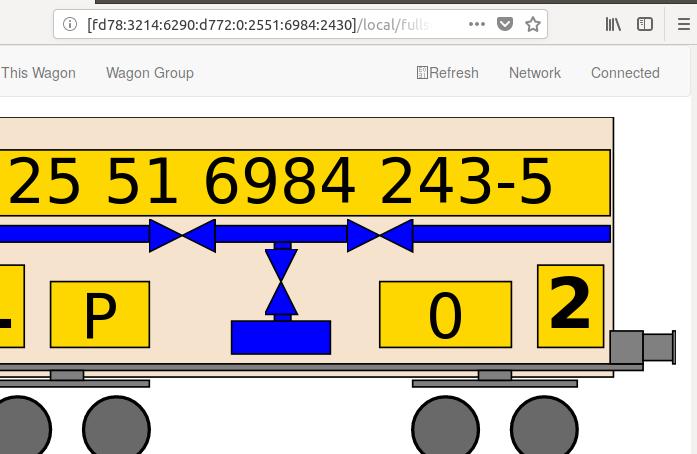
\includegraphics[width=\textwidth]{Bilder/ipv6_concept.png}
    \caption{Mögliche Darstellung des virtuellen Güterwagens mit IPv6-Netzwerkadresse\cite{GAK}}
    \label{fig:IPv6}
\end{figure}
Alle Wagen sollen hierarchisch gleich gestellt sein. außerdem darf keine Abhängigkeit zu Netzwerkverbindungen oder Servern bestehen. Darum soll durch Dezentralität und lokalen Netzwerken immer eine lokale Verbindung bestehen. In dieser wird eine lokale Hierarchie gebildet.\par
Im Verband mit anderen Wagen verhält sich der Güterwagen 4.0 sozial und teilt alle notwendigen Informationen über sicht mit den anderen Wagen und der lok als gleichberechtigte Partner. Dazu gehören bauartspezifische Parameter wie Gewicht, Länge, Achszahl, maximal Zuladung und Höchstgeschwindigkeit genauso wie wagen spezifische Informationen wie Besitzer, Laufleistung, Informationen aus den Sensoren, letzte Wartungen und nächste Instandhaltungszyklen.\par
Aufgrund der vielen unterschiedlich konfigurierten Güterwagen und Zugängen zu Daten und Akten wird eine NoSQL-Technologie als Datenbankformat gewählt. Diese sorgt auch bei unterschiedlichen Versionen und Daten für eine zukunftssichere Datenbank.\par
Eine weitere Beschreibung des Bordrechners ist in Kapitel \ref{sec:eKomp} zu finden, die Beschreibung der Kommunikation in Kapitel \ref{sec:dKomp} zu finden.



    \subsection{Realisierung elektrischer Komponenten}\label{sec:eKomp}
In diesem Kapitel werden die elektrischen Komponenten einzeln beschrieben. Dieses Kapitel ist zugehörig zum Arbeitspaket 3 - Entwicklung Aktorik; genauer AP 3a: Konzeptentwicklung Aktorik und Aktorsteuerung und behandelt den die elektrischen Komponenten; die pneumatischen Aktoren werden im folgenden Kapitel beschrieben.\par
Die elektrischen Komponenten sind in Abbildung \ref{fig:eKomp} farblich hervorgehoben.
Für den Demonstrator sind drei große, elektrische Module geplant: Batterie, Bordelektronik und die Ladeelektronik, bestehend aus dem Radsatzgenerator und einer Ladeschnittstelle zur externen Aufladung (alle in blau dargestellt). Zusätzlich müssen auch alle weiteren Aktoren und Sensoren sowie Datenschnittstellen außerhalb dieser Elektronik mit Spannung versorgt werden (hier in schwarz gestrichelt dargestellt).\par
\begin{figure}[hbt]
    \centering
    \pgfdeclarelayer{background}
\pgfdeclarelayer{foreground}
\pgfdeclarelayer{Beschriftung}
%Farbendefinition
\definecolor{elek}{RGB}{55,126,184}%blau
\definecolor{pneu}{RGB}{105,105,105}%grau
\definecolor{sens}{RGB}{105,105,105}%grau
\definecolor{dat}{RGB}{105,105,105}%grau
\definecolor{strom}{RGB}{0,0,0}%schwarz

\tikzset{wagon/.style={draw = gray, ultra thick, opacity = 0.7}}
\tikzset{seite/.style={opacity = 1}}
\tikzset{elek/.style= {draw = elek, ultra thick, opacity = 1}} %elektrische Komponenten
\tikzset{sens/.style={draw = sens, ultra thick, opacity = 1}} %sensorische Komponenten
\tikzset{pneu/.style={draw = pneu, ultra thick, opacity = 1}} %pneumatische Komponenten
\tikzset{dat/.style={draw = dat, ultra thick, opacity = 1}} %Datenkomponenten
\tikzset{strom/.style={draw = strom, ultra thick, opacity = 1}} %Strom- und Datenleitungen
\tikzset{annotation/.style={draw = black, thick, opacity = 0.7, font=\scriptsize}}

\pgfsetlayers{background,main,Beschriftung,foreground}
\begin{tikzpicture}[scale=0.7]
%%%%%%%%%%%%%%%%%%%%%%%%%%%%%%%%%%%%%%%%%%%%%%%% Hintergrund %%%%%%%%%%%%%%%%%%%%%%%%%%%%%%%%%%%%%%%%%%%%%
    \begin{pgfonlayer}{background}
    %Seiten
        %Seite A
        \path[seite] (-6, 3) rectangle +(.6,.2) node[pos = 0.5] (seiteA) {Seite A};
        %Seite B
        \path[seite] (5.3, 3) rectangle +(.6,.2) node[pos = 0.5] (seiteB) {Seite B};
    %wagon als Basis
    \path[wagon] (-5,-2) -- (-5,2) -- (5,2) -- (5,-2) -- cycle;
    % HL
    \path[wagon, color=pneu] (-5,-.5) -- (5,-.5) node[pos = 0.6, above] {\color=\gray \tiny{HLL}};
    % Buffer
    \begin{scope}[shift = {(-5,1.5)}]
    	\path[wagon] (-.8,.3) -- (0,.3) -- (0,-.3) -- (-.8,-.3);
    	\path[wagon] (-1,.25) -- (-.8,.25) -- (-.8,-.25) -- (-1,-.25);
    	\path[wagon] (-1,-.5) .. controls (-1.05,0) and (-1.05,0) .. (-1,.5);
    \end{scope}
    \begin{scope}[shift = {(-5,-1.5)}]
    	\path[wagon] (-.8,.3) -- (0,.3) -- (0,-.3) -- (-.8,-.3);
    	\path[wagon] (-1,.25) -- (-.8,.25) -- (-.8,-.25) -- (-1,-.25);
    	\path[wagon] (-1,-.5) .. controls (-1.05,0) and (-1.05,0) .. (-1,.5);
    \end{scope}
    \begin{scope}[shift = {(5,-1.5)}, rotate = 180]
    	\path[wagon] (-.8,.3) -- (0,.3) -- (0,-.3) -- (-.8,-.3);
    	\path[wagon] (-1,.25) -- (-.8,.25) -- (-.8,-.25) -- (-1,-.25);
    	\path[wagon] (-1,-.5) .. controls (-1.05,0) and (-1.05,0) .. (-1,.5);
    \end{scope}
    \begin{scope}[shift = {(5,1.5)}, rotate = 180]
    	\path[wagon] (-.8,.3) -- (0,.3) -- (0,-.3) -- (-.8,-.3);
    	\path[wagon] (-1,.25) -- (-.8,.25) -- (-.8,-.25) -- (-1,-.25);
    	\path[wagon] (-1,-.5) .. controls (-1.05,0) and (-1.05,0) .. (-1,.5);
    \end{scope}
    %Wheelset
    \begin{scope}[shift = {(-4,0)}]
    	\path[wagon] (-.1,1.7) -- (.1,1.7) -- (.1,-1.7) -- (-.1, -1.7) -- cycle; 
    	\path[wagon] (-.6,1.4) -- (.6,1.4) -- (.55,1.5) -- (-.55, 1.5) -- cycle; 
    	\path[wagon] (-.6,-1.4) -- (.6,-1.4) -- (.55,-1.5) -- (-.55, -1.5) -- cycle; 
    \end{scope}
        \begin{scope}[shift = {(-2.5,0)}]
    	\path[wagon] (-.1,1.7) -- (.1,1.7) -- (.1,-1.7) -- (-.1, -1.7) -- cycle; 
    	\path[wagon] (-.6,1.4) -- (.6,1.4) -- (.55,1.5) -- (-.55, 1.5) -- cycle; 
    	\path[wagon] (-.6,-1.4) -- (.6,-1.4) -- (.55,-1.5) -- (-.55, -1.5) -- cycle; 
    \end{scope}
    \begin{scope}[shift = {(4,0)}]
    	\path[wagon] (-.1,1.7) -- (.1,1.7) -- (.1,-1.7) -- (-.1, -1.7) -- cycle; 
    	\path[wagon] (-.6,1.4) -- (.6,1.4) -- (.55,1.5) -- (-.55, 1.5) -- cycle; 
    	\path[wagon] (-.6,-1.4) -- (.6,-1.4) -- (.55,-1.5) -- (-.55, -1.5) -- cycle; 
    \end{scope}
    \begin{scope}[shift = {(2.5,0)}]
    	\path[wagon] (-.1,1.7) -- (.1,1.7) -- (.1,-1.7) -- (-.1, -1.7) -- cycle; 
    	\path[wagon] (-.6,1.4) -- (.6,1.4) -- (.55,1.5) -- (-.55, 1.5) -- cycle; 
    	\path[wagon] (-.6,-1.4) -- (.6,-1.4) -- (.55,-1.5) -- (-.55, -1.5) -- cycle; 
    \end{scope}
    \end{pgfonlayer}
%%%%%%%%%%%%%%%%%%%%%%%%%%%%%%%%%%%%%%%%%%%%%%% Vordergrung %%%%%%%%%%%%%%%%%%%%%%%%%%%%%%%%%%%%%%%%%%%%%%%%%
    \begin{pgfonlayer}{foreground} %Komponete
    %elektronische Komponenten
        %Radsatzgenerator
        \path[elek, fill = elek, thin] (-4.3, -1.9) rectangle +(.6,.2) node[pos = 0.5] (wsg) {};
        %Rechner
        \path[elek, fill = elek, thin] (-.5, -1.6) rectangle +(1,.3) node[pos = 0.5] (bcu) {};
        %Batterie
        \path[elek, fill = elek, thin] (-1.8, -1.8) rectangle +(1,.5) node[pos = 0.5] (bat) {};
        %optionale Ladeelektronik
        \path[elek, fill = elek, thin] (-1.8, 1.2) rectangle +(0.8,.4) node[pos = 0.5] (ole) {};
    % pneumatische Komponenten
        %epBremse
        \path[pneu, fill = pneu] (.9,-1.3) rectangle (1.1,-1.5) node[pos = 0.5] (epb) {};
        %Endabsperrhähne
        \path[pneu, fill = pneu] (-5.2, -.4) rectangle (-5,-.6) node[pos = 0.5] (eca) {};
        \path[pneu, fill = pneu] (5.2, -.4) rectangle (5,-.6) node[pos = 0.5] (ecb) {};
        %Aktorik Bremse
        \path[pneu, fill = pneu, thin] (-.5, 0) rectangle +(1,.5) node[pos = 0.5] (bcu2) {};
    %sensorische Komponenten
        %drahtloserSensor
        \path[sens, fill = sens, thin] (3.9, -1.7) rectangle +(.2,-.2) node[pos = 0.5] (wss) {};
        %Flachstellendektektor
        \path[sens, fill=sens, thin] (3.15, 1.8) rectangle +(.2,-.2) node[pos = 0.5] (flachstelle) {};
        \path[sens, fill=sens, thin] (-3.35, 1.8) rectangle +(.2,-.2) node[pos = 0.5] (flachstelle2) {};
        %Laufleistung
        \path[sens, fill = sens, thin] (3.9, 0) rectangle +(.2,-.2) node[pos = 0.5] (ll) {};
    %Datenkomponeten
        %Kurzstreckenfunk
        \path[dat, fill = dat] (-5.2, -.9) rectangle (-5,-1.05)node[pos = 0.5] (sra) {};
        \path[dat, fill = dat] (5.2, -.9) rectangle (5,-1.05)node[pos = 0.5] (srb) {};
        \path[dat, fill = dat] (5.2, .9) rectangle (5,1.05)node[pos = 0.5] (src) {};
        \path[dat, fill = dat] (-5.2, .9) rectangle (-5,1.05) node[pos = 0.5] (srd) {};
    \end{pgfonlayer}
%%%%%%%%%%%%%%%%%%%%%%%%%%%%%%%%%%%%%%%%%%%%%%% Beschriftung %%%%%%%%%%%%%%%%%%%%%%%%%%%%%%%%%%%%%%%%%%%%%%%%%
    \begin{pgfonlayer}{Beschriftung}
    %elektronische Komponenten
        %Radsatzgenerator
        \path[annotation, thin] (wsg) -- +(-.5,-.5) node[left] {Achsdeckelgenerator};
        %Rechner
        \path[annotation, thin] (bcu) -- +(1,-1) node[right] {Bordelektronik};
        %Batterie
        \path[annotation, thin] (bat) -- +(-1,-1) node[left] {Batterie};
        %optionale Ladeelektronik
        \path[annotation, thin] (ole) -- +(-.9,.9) node[left] {externe Ladeschnittstelle};
    %pneumatische Komponenten
        %epBremse
        \path[annotation, thin] (epb) -- +(.4,-.4) node[right] {ep-Bremse};
        %Endabsperrhähne
        \path[annotation, thin] (eca) -- +(-.5,.5) node[left] {Aktor Endabsperrhahn};
        %Aktorik Bremse
        \path[annotation, thin] (bcu2) -- +(.5,.5) node[right] {Aktorik Bremse};
    %sensorische Komponenten
        %drahtloserSensor
        \path[annotation, thin] (wss) -- +(.5,-.5) node[right] {Laufleistung}; 
        %Flachstellen
        \path[annotation, thin] (flachstelle) -- +(.7,.7) node[right] {Lagertemperatur};
        \path[annotation, thin] (flachstelle2) -- +(7.2,.7) node[right] {};
        %Laufleistung
        \path[annotation, thin] (ll) -- +(1.2,.5) node[right] {Beschleunigungen};
    %Datenkomponeten
        %Kurzstreckenfunk
        \path[annotation, thin] (srd) -- +(-.5,-.5) node[left] {Kurzstreckenfunk};    
    \end{pgfonlayer}
%%%%%%%%%%%%%%%%%%%%%%%%%%%%%%%%%%%%%%%%%%%%%% Main %%%%%%%%%%%%%%%%%%%%%%%%%%%%%%%%%%%%%%%%%%%%%%%%%%%%
    \begin{pgfonlayer}{main} %Leitungen
    %elek
        %Radsatzgenerator
        \path[elek] (wsg) +(-.1,0) -| (-3.3, -1);%-- +(1,0) -- (-3.2,-1);
        \path[strom, dashed] (wsg) +(-.1,0) -| (-3.3, -1);%-- +(1,0) -- (-3.2,-1);
        %Rechner
        \path[elek] (bcu) +(0,0)  -- (0,-1);
        \path[strom, dashed] (bcu) +(0,0)  -- (0,-1);
        %Batterie
        \path[elek] (bat) +(0,0)  -- (-1.3,-1);
        \path[strom, dashed] (bat) +(0,0)  -- (-1.3,-1);
        %optionale Ladeelektronik
        \path[elek] (ole) +(0,0)  -- (-1.35,-1);
        \path[strom, dashed] (ole) +(0,0)  -- (-1.35,-1);
    %pneu
        %ep-Bremse
        \path[pneu] (1,-.5) -- (1,-1.3);
        %\path[strom, dashed] (1,-.5) -- (1,-1.3);
        \path[pneu] (epb) +(.1,0) -- +(-.5,0);
        \path[strom, dashed] (epb) +(.1,0) -- +(-.5,0);
        %Endabsperrhähne
        \path[pneu] (eca) +(-.1,0) -- +(.2,0) -- (-4.9,-1);
        \path[strom, dashed] (eca) +(-.1,0) -- +(.2,0) -- (-4.9,-1);
        \path[pneu] (ecb) +(.1,0) -- +(-.2,0) -- (4.9,-1);
        \path[strom, dashed] (ecb) +(.1,0) -- +(-.2,0) -- (4.9,-1);
        %Aktorik Bremse
        \path[pneu] (bcu2) +(0,0)  -- (0,-1);
        \path[strom, dashed] (bcu2) +(0,0)  -- (0,-1);
    %Sensorische Kompoenten
        %Flachstellen
        \path[sens] (flachstelle)+(0,0) -- (3.2, -1);
        \path[strom, dashed] (flachstelle)+(0,0) -- (3.2, -1);
        \path[sens] (flachstelle2) +(0,0)-- (-3.3, -1);
        \path[strom, dashed] (flachstelle2) +(0,0)-- (-3.3, -1);
        %Laufleistung
        \path[sens] (ll)+(0,0) -- (4, -1);
        \path[strom, dashed] (ll)+(0,0) -- (4, -1);
        %drahloser Sensor
        \path[strom, dotted] (wss)+(0,0) -- (4, -1);
    %Strom- und Datenleitung
        \path[dat] (-5,-1) -- (5,-1);
        \path[strom, dashed] (-5,-1) -- (5,-1);
        %Kurzstreckenfunk
        \path[dat] (srd) +(-.1,0) -- +(.3,0) -- (-4.8,-1);
        \path[strom, dashed] (srd) +(-.1,0) -- +(.3,0) -- (-4.8,-1);
        \path[dat] (src) +(.1,0) -- +(-.3,0) -- (4.8,-1);
        \path[strom, dashed] (src) +(.1,0) -- +(-.3,0) -- (4.8,-1);
    \end{pgfonlayer}

\end{tikzpicture}

    \caption{elektrische Komponenten des Gesamtsystems}
    \label{fig:eKomp}
\end{figure}
Für den serienreifen Güterwagen 4.0 ist auch eine Aufladung der Batterie durch eine Automatische Kupplung oder fest verlegte Kabel denkbar, diese sollen für den \gls{Demonstrator} aber noch nicht betrachtet werden.

\paragraph{Achsdeckelgenerator} \label{sec:RSG}
Das elektrische Konzept sieht vor, dass ein Radsatz- oder Achsdeckelgenerator im Umlauf des Wagens genug Energie produziert um alle notwendigen Komponenten zu speisen sowie zusätzlich eine Pufferbatterie für den geplanten und ungeplanten Fall des Stillstandes lädt.
\paragraph{Externe Ladeschnittstelle}
Zur Aufladung der Systembatterie im Stillstand wird eine externe Ladeschnittstelle benötigt. Diese ist auch für Lokomotiven üblich und soll übernommen werden. Für die Demonstratoren ist sie besonders wichtig, da sie keinen Üblichen Umlauf fahren.
\paragraph{Batterie}\label{sec:Batterie}
Die Batterie benötigt genügend Leistung für eine übliche Speisung der Bord- elektronik, der Aktoren und Sensoren sowie einen Puffer bei ungeplanten Zeitverzöger- ungen.
\paragraph{Bordelektronik}
Die Bordelektronik steuert alle für den Güterwagen notwendigen Prozesse. Dazu gehören sichere und nicht sichere Prozesse.\par
Bei sicheren Prozessen wird von außen reiner Lesezugriff gewährt. Bei nicht sicheren Funktionen ist auch ein Schreibrecht von außen zu geben. Siehe dazu auch Die Systemarchitektur des Rechners im Kapitel \ref{sec:dKomp}.\par
Zu den sicheren Funktionen gehören:
\begin{itemize}
    \item Steuerung der pneumatischen und elektrischen Aktoren,
    \item Kommunikation mit den Sensoren,
    \item Speicherung der Daten der Sensoren,
    \item Steuerung und Regelung des Lademanagments,
    \item Kommunikation mit anderen Güterwagen 4.0 Lokomotiven.
\end{itemize}
Nicht sichere Funktionen dagegen können von außen im Stand und von entsprechen autorisierten Personen beschrieben werden. Zu diesen gehören:
\begin{itemize}
    \item Kommunikation mit dem Bediener
    \item Speicherung weiterer Informationen über den Güterwagen,
    \item Kommunikation mit der Cloud zur Aktualisierung des 'Digitalen Zwillings'.
\end{itemize}
















    \subsection{Realisierung pneumatischer Komponenten}
In diesem Kapitel werden die pneumatischen Komponenten einzeln beschrieben. Dieses Kapitel ist zugehörig zum Arbeitspaket 3 - Entwicklung Aktorik; genauer AP 3a: Konzeptentwicklung Aktorik und Aktorsteuerung und behandelt die (pneumatischen) Aktoren.\par
Die pneumatischen Komponenten sind in Abbildung \ref{fig:pKomp} in grün farblich hervorgehoben.\par
Für den Demonstrator ist eine teilautomatisierte Bremssteuerung geplant. Diese beinhaltet die Aktorik des Güterwagens 4.0; siehe dazu auch Abbildung \ref{fig:UIC-Bremse} auf \pageref{fig:UIC-Bremse}. Diese Bremse besteht neben dem unangetasteten UIC-Steuerventil und den unangetasteten A- und R-Kammern auch aus einigen Aktoren.\par
\begin{figure}[hbt]
    \centering
    \pgfdeclarelayer{background}
\pgfdeclarelayer{foreground}
\pgfdeclarelayer{Beschriftung}
%Farbendefinition
\definecolor{elek}{RGB}{105,105,105}%grau{55,126,184}%blau
\definecolor{pneu}{RGB}{77,175,74}%grün{pneu}{RGB}{105,105,105}%grau
\definecolor{sens}{RGB}{105,105,105}%grau
\definecolor{dat}{RGB}{105,105,105}%grau
\definecolor{strom}{RGB}{105,105,105}%grau %{0,0,0}%schwarz

\tikzset{wagon/.style={draw = gray, ultra thick, opacity = 0.7}}
\tikzset{seite/.style={opacity = 1}}
\tikzset{elek/.style= {draw = elek, ultra thick, opacity = 1}} %elektrische Komponenten
\tikzset{sens/.style={draw = sens, ultra thick, opacity = 1}} %sensorische Komponenten
\tikzset{pneu/.style={draw = pneu, ultra thick, opacity = 1}} %pneumatische Komponenten
\tikzset{dat/.style={draw = dat, ultra thick, opacity = 1}} %Datenkomponenten
\tikzset{strom/.style={draw = strom, ultra thick, opacity = 1}} %Strom- und Datenleitungen
\tikzset{annotation/.style={draw = black, thick, opacity = 0.7, font=\scriptsize}}

\pgfsetlayers{background,main,Beschriftung,foreground}
\begin{tikzpicture}[scale=0.7]
%%%%%%%%%%%%%%%%%%%%%%%%%%%%%%%%%%%%%%%%%%%%%%%% Hintergrund %%%%%%%%%%%%%%%%%%%%%%%%%%%%%%%%%%%%%%%%%%%%%
    \begin{pgfonlayer}{background}
    %Seiten
        %Seite A
        \path[seite] (-6, 3) rectangle +(.6,.2) node[pos = 0.5] (seiteA) {Seite A};
        %Seite B
        \path[seite] (5.3, 3) rectangle +(.6,.2) node[pos = 0.5] (seiteB) {Seite B};
    %wagon als Basis
    \path[wagon] (-5,-2) -- (-5,2) -- (5,2) -- (5,-2) -- cycle;
    % HL
    \path[wagon, color=pneu] (-5,-.5) -- (5,-.5) node[pos = 0.6, above] {\color=\gray \tiny{HLL}};
    % Buffer
    \begin{scope}[shift = {(-5,1.5)}]
    	\path[wagon] (-.8,.3) -- (0,.3) -- (0,-.3) -- (-.8,-.3);
    	\path[wagon] (-1,.25) -- (-.8,.25) -- (-.8,-.25) -- (-1,-.25);
    	\path[wagon] (-1,-.5) .. controls (-1.05,0) and (-1.05,0) .. (-1,.5);
    \end{scope}
    \begin{scope}[shift = {(-5,-1.5)}]
    	\path[wagon] (-.8,.3) -- (0,.3) -- (0,-.3) -- (-.8,-.3);
    	\path[wagon] (-1,.25) -- (-.8,.25) -- (-.8,-.25) -- (-1,-.25);
    	\path[wagon] (-1,-.5) .. controls (-1.05,0) and (-1.05,0) .. (-1,.5);
    \end{scope}
    \begin{scope}[shift = {(5,-1.5)}, rotate = 180]
    	\path[wagon] (-.8,.3) -- (0,.3) -- (0,-.3) -- (-.8,-.3);
    	\path[wagon] (-1,.25) -- (-.8,.25) -- (-.8,-.25) -- (-1,-.25);
    	\path[wagon] (-1,-.5) .. controls (-1.05,0) and (-1.05,0) .. (-1,.5);
    \end{scope}
    \begin{scope}[shift = {(5,1.5)}, rotate = 180]
    	\path[wagon] (-.8,.3) -- (0,.3) -- (0,-.3) -- (-.8,-.3);
    	\path[wagon] (-1,.25) -- (-.8,.25) -- (-.8,-.25) -- (-1,-.25);
    	\path[wagon] (-1,-.5) .. controls (-1.05,0) and (-1.05,0) .. (-1,.5);
    \end{scope}
    %Wheelset
    \begin{scope}[shift = {(-4,0)}]
    	\path[wagon] (-.1,1.7) -- (.1,1.7) -- (.1,-1.7) -- (-.1, -1.7) -- cycle; 
    	\path[wagon] (-.6,1.4) -- (.6,1.4) -- (.55,1.5) -- (-.55, 1.5) -- cycle; 
    	\path[wagon] (-.6,-1.4) -- (.6,-1.4) -- (.55,-1.5) -- (-.55, -1.5) -- cycle; 
    \end{scope}
        \begin{scope}[shift = {(-2.5,0)}]
    	\path[wagon] (-.1,1.7) -- (.1,1.7) -- (.1,-1.7) -- (-.1, -1.7) -- cycle; 
    	\path[wagon] (-.6,1.4) -- (.6,1.4) -- (.55,1.5) -- (-.55, 1.5) -- cycle; 
    	\path[wagon] (-.6,-1.4) -- (.6,-1.4) -- (.55,-1.5) -- (-.55, -1.5) -- cycle; 
    \end{scope}
    \begin{scope}[shift = {(4,0)}]
    	\path[wagon] (-.1,1.7) -- (.1,1.7) -- (.1,-1.7) -- (-.1, -1.7) -- cycle; 
    	\path[wagon] (-.6,1.4) -- (.6,1.4) -- (.55,1.5) -- (-.55, 1.5) -- cycle; 
    	\path[wagon] (-.6,-1.4) -- (.6,-1.4) -- (.55,-1.5) -- (-.55, -1.5) -- cycle; 
    \end{scope}
    \begin{scope}[shift = {(2.5,0)}]
    	\path[wagon] (-.1,1.7) -- (.1,1.7) -- (.1,-1.7) -- (-.1, -1.7) -- cycle; 
    	\path[wagon] (-.6,1.4) -- (.6,1.4) -- (.55,1.5) -- (-.55, 1.5) -- cycle; 
    	\path[wagon] (-.6,-1.4) -- (.6,-1.4) -- (.55,-1.5) -- (-.55, -1.5) -- cycle; 
    \end{scope}
    \end{pgfonlayer}
%%%%%%%%%%%%%%%%%%%%%%%%%%%%%%%%%%%%%%%%%%%%%%% Vordergrung %%%%%%%%%%%%%%%%%%%%%%%%%%%%%%%%%%%%%%%%%%%%%%%%%
    \begin{pgfonlayer}{foreground} %Komponete
    %elektronische Komponenten
        %Radsatzgenerator
        \path[elek, fill = elek, thin] (-4.3, -1.9) rectangle +(.6,.2) node[pos = 0.5] (wsg) {};
        %Rechner
        \path[elek, fill = elek, thin] (-.5, -1.6) rectangle +(1,.3) node[pos = 0.5] (bcu) {};
        %Batterie
        \path[elek, fill = elek, thin] (-1.8, -1.8) rectangle +(1,.5) node[pos = 0.5] (bat) {};
        %optionale Ladeelektronik
        \path[elek, fill = elek, thin] (-1.8, 1.2) rectangle +(0.8,.4) node[pos = 0.5] (ole) {};
    % pneumatische Komponenten
        %epBremse
        \path[pneu, fill = pneu] (.9,-1.3) rectangle (1.1,-1.5) node[pos = 0.5] (epb) {};
        %Endabsperrhähne
        \path[pneu, fill = pneu] (-5.2, -.4) rectangle (-5,-.6) node[pos = 0.5] (eca) {};
        \path[pneu, fill = pneu] (5.2, -.4) rectangle (5,-.6) node[pos = 0.5] (ecb) {};
        %Aktorik Bremse
        \path[pneu, fill = pneu, thin] (-.5, 0) rectangle +(1,.5) node[pos = 0.5] (bcu2) {};
    %sensorische Komponenten
        %drahtloserSensor
        \path[sens, fill = sens, thin] (3.9, -1.7) rectangle +(.2,-.2) node[pos = 0.5] (wss) {};
        %Flachstellendektektor
        \path[sens, fill=sens, thin] (3.15, 1.8) rectangle +(.2,-.2) node[pos = 0.5] (flachstelle) {};
        \path[sens, fill=sens, thin] (-3.35, 1.8) rectangle +(.2,-.2) node[pos = 0.5] (flachstelle2) {};
        %Laufleistung
        \path[sens, fill = sens, thin] (3.9, 0) rectangle +(.2,-.2) node[pos = 0.5] (ll) {};
    %Datenkomponeten
        %Kurzstreckenfunk
        \path[dat, fill = dat] (-5.2, -.9) rectangle (-5,-1.05)node[pos = 0.5] (sra) {};
        \path[dat, fill = dat] (5.2, -.9) rectangle (5,-1.05)node[pos = 0.5] (srb) {};
        \path[dat, fill = dat] (5.2, .9) rectangle (5,1.05)node[pos = 0.5] (src) {};
        \path[dat, fill = dat] (-5.2, .9) rectangle (-5,1.05) node[pos = 0.5] (srd) {};
    \end{pgfonlayer}
%%%%%%%%%%%%%%%%%%%%%%%%%%%%%%%%%%%%%%%%%%%%%%% Beschriftung %%%%%%%%%%%%%%%%%%%%%%%%%%%%%%%%%%%%%%%%%%%%%%%%%
    \begin{pgfonlayer}{Beschriftung}
    %elektronische Komponenten
        %Radsatzgenerator
        \path[annotation, thin] (wsg) -- +(-.5,-.5) node[left] {Achsdeckelgenerator};
        %Rechner
        \path[annotation, thin] (bcu) -- +(1,-1) node[right] {Bordelektronik};
        %Batterie
        \path[annotation, thin] (bat) -- +(-1,-1) node[left] {Batterie};
        %optionale Ladeelektronik
        \path[annotation, thin] (ole) -- +(-.9,.9) node[left] {externe Ladeschnittstelle};
    %pneumatische Komponenten
        %epBremse
        \path[annotation, thin] (epb) -- +(.4,-.4) node[right] {ep-Bremse};
        %Endabsperrhähne
        \path[annotation, thin] (eca) -- +(-.5,.5) node[left] {Aktor Endabsperrhahn};
        %Aktorik Bremse
        \path[annotation, thin] (bcu2) -- +(.5,.5) node[right] {Aktorik Bremse};
    %sensorische Komponenten
        %drahtloserSensor
        \path[annotation, thin] (wss) -- +(.5,-.5) node[right] {Laufleistung}; 
        %Flachstellen
        \path[annotation, thin] (flachstelle) -- +(.7,.7) node[right] {Lagertemperatur};
        \path[annotation, thin] (flachstelle2) -- +(7.2,.7) node[right] {};
        %Laufleistung
        \path[annotation, thin] (ll) -- +(1.2,.5) node[right] {Beschleunigungen};
    %Datenkomponeten
        %Kurzstreckenfunk
        \path[annotation, thin] (srd) -- +(-.5,-.5) node[left] {Kurzstreckenfunk};    
    \end{pgfonlayer}
%%%%%%%%%%%%%%%%%%%%%%%%%%%%%%%%%%%%%%%%%%%%%% Main %%%%%%%%%%%%%%%%%%%%%%%%%%%%%%%%%%%%%%%%%%%%%%%%%%%%
    \begin{pgfonlayer}{main} %Leitungen
    %elek
        %Radsatzgenerator
        \path[elek] (wsg) +(-.1,0) -| (-3.3, -1);%-- +(1,0) -- (-3.2,-1);
        \path[strom, dashed] (wsg) +(-.1,0) -| (-3.3, -1);%-- +(1,0) -- (-3.2,-1);
        %Rechner
        \path[elek] (bcu) +(0,0)  -- (0,-1);
        \path[strom, dashed] (bcu) +(0,0)  -- (0,-1);
        %Batterie
        \path[elek] (bat) +(0,0)  -- (-1.3,-1);
        \path[strom, dashed] (bat) +(0,0)  -- (-1.3,-1);
        %optionale Ladeelektronik
        \path[elek] (ole) +(0,0)  -- (-1.35,-1);
        \path[strom, dashed] (ole) +(0,0)  -- (-1.35,-1);
    %pneu
        %ep-Bremse
        \path[pneu] (1,-.5) -- (1,-1.3);
        %\path[strom, dashed] (1,-.5) -- (1,-1.3);
        \path[pneu] (epb) +(.1,0) -- +(-.5,0);
        \path[strom, dashed] (epb) +(.1,0) -- +(-.5,0);
        %Endabsperrhähne
        \path[pneu] (eca) +(-.1,0) -- +(.2,0) -- (-4.9,-1);
        \path[strom, dashed] (eca) +(-.1,0) -- +(.2,0) -- (-4.9,-1);
        \path[pneu] (ecb) +(.1,0) -- +(-.2,0) -- (4.9,-1);
        \path[strom, dashed] (ecb) +(.1,0) -- +(-.2,0) -- (4.9,-1);
        %Aktorik Bremse
        \path[pneu] (bcu2) +(0,0)  -- (0,-1);
        \path[strom, dashed] (bcu2) +(0,0)  -- (0,-1);
    %Sensorische Kompoenten
        %Flachstellen
        \path[sens] (flachstelle)+(0,0) -- (3.2, -1);
        \path[strom, dashed] (flachstelle)+(0,0) -- (3.2, -1);
        \path[sens] (flachstelle2) +(0,0)-- (-3.3, -1);
        \path[strom, dashed] (flachstelle2) +(0,0)-- (-3.3, -1);
        %Laufleistung
        \path[sens] (ll)+(0,0) -- (4, -1);
        \path[strom, dashed] (ll)+(0,0) -- (4, -1);
        %drahloser Sensor
        \path[strom, dotted] (wss)+(0,0) -- (4, -1);
    %Strom- und Datenleitung
        \path[dat] (-5,-1) -- (5,-1);
        \path[strom, dashed] (-5,-1) -- (5,-1);
        %Kurzstreckenfunk
        \path[dat] (srd) +(-.1,0) -- +(.3,0) -- (-4.8,-1);
        \path[strom, dashed] (srd) +(-.1,0) -- +(.3,0) -- (-4.8,-1);
        \path[dat] (src) +(.1,0) -- +(-.3,0) -- (4.8,-1);
        \path[strom, dashed] (src) +(.1,0) -- +(-.3,0) -- (4.8,-1);
    \end{pgfonlayer}

\end{tikzpicture}

    \caption{Pneumatische Komponenten des Gesamtsystems}
    \label{fig:pKomp}
\end{figure}
Alle Aktoren sollen, für eine vereinfachte Zulassung, vor Fahrtantritt abschaltbar sein. Damit sie in der geforderten Position bleiben werden bistabile Magnetventile benötigt. Diese halten sicher ihre Stellung auch ohne Stromversorgung. So ist nur darüber ein Nachweis zu führen.
\begin{figure}
    \centering%[hbt]
    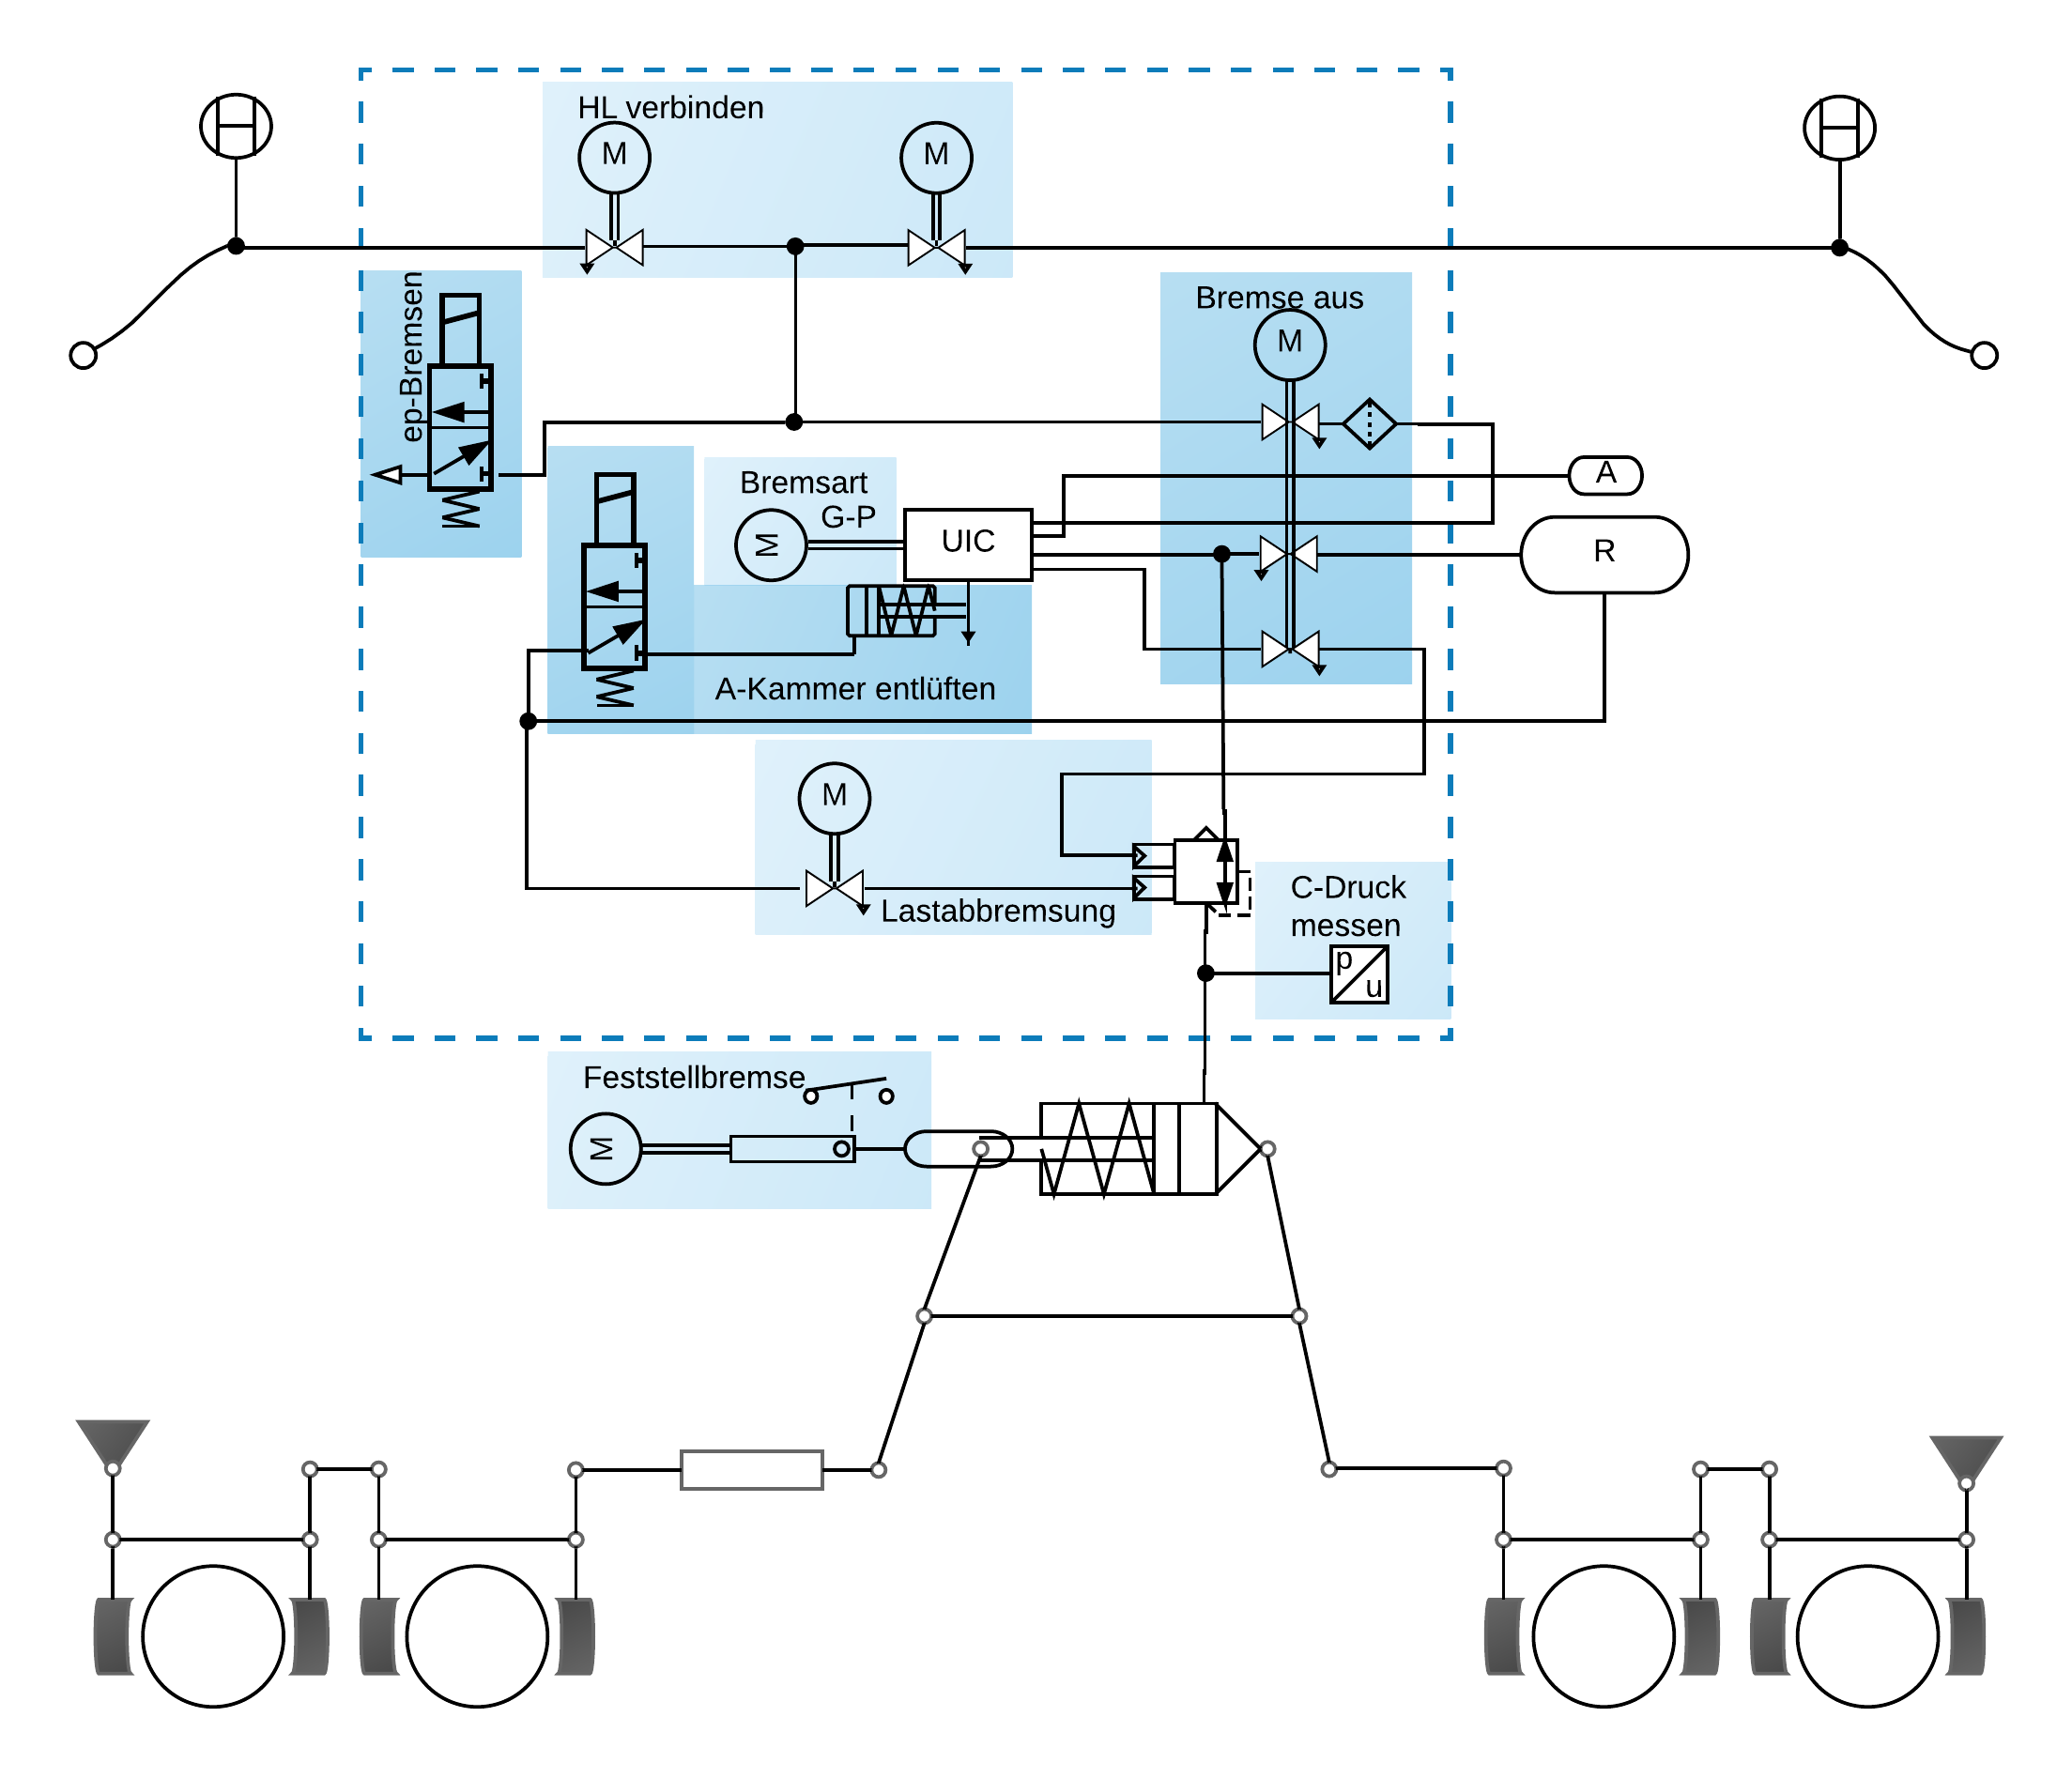
\includegraphics[width=10cm%\textwidth
    ]{Bilder/Abb3_Druckluftbremse.png}
    \caption{UIC-kompatible Druckluftbremse des Güterwagen 4.0 \cite{ETR_2}}
    \label{fig:UIC-Bremse}
\end{figure}

\paragraph{Steuerventil}\label{sec:Bremsart}
Aus Zulassungsgründen wird ein UIC/TSI-kompatibles Steuerventil eingesetzt oder beibehalten. Dieses unterstützt die folgenden Funktionen: Bremsstellung zwischen G und P wechseln und automatisches Schnelllösen

\paragraph{Relaisventil} Es gibt ein Relaisventil zur automatischen Lastabbremsung.

\paragraph{Endabsperrhahn} \label{sec:Endabsperrhahn}
An beiden Enden des Wagens werden die Endabsperrhähne mit zu- sätzliche Ventilen ausgestattet. Diese sorgen für eine sichere Trennung und Kupplung von Wagen durch automatisches öffnen und schließen. Zusätzlich bieten sie eine wichtige Unterstützung zur automatischen Bremsprobe, da sie direkt ansteuerbar sind.

%\paragraph{Bremsartumsteller} 
%Der Bremsartumsteller bietet eine einfache Umstellung zwischen den Bremsarten. So ist das Umstellen der Bremsart G in P auf Befehl möglich.

\paragraph{Feststellbremse}
Durch die Einführung der automatischen Feststellbremse fällt das legen von Hemmschuhen vor dem Wagen weg. \\?

\paragraph{ep-assist-Bremse} 
Ein ep-Bremsventil wird mit der Hauptluftleitung verbunden. \gls{ep-assist-Bremsen}



    \subsection{Realisierung sensorischer Komponenten}
In diesem Kapitel werden die sensorischen Komponenten einzeln beschrieben. Dieses Kapitel ist zugehörig zum Arbeitspaket 4 - Entwicklung Sensorik; genauer AP 4a: Konzeptentwicklung Sensorik und behandelt den sensorischen Teil des Güterwagen 4.0 inklusive Condition Monitoring.\par
Die sensorischen Komponenten sind in Abbildung \ref{fig:sKomp} in rot farblich aufgezeigt.
\begin{figure}[hbt]
    \centering
    \pgfdeclarelayer{background}
\pgfdeclarelayer{foreground}
\pgfdeclarelayer{Beschriftung}
%Farbendefinition
\definecolor{elek}{RGB}{105,105,105}%grau{55,126,184}%blau
\definecolor{pneu}{RGB}{105,105,105}%grau
\definecolor{sens}{RGB}{228,26,28}%rot{105,105,105}%grau
\definecolor{dat}{RGB}{105,105,105}%grau
\definecolor{strom}{RGB}{105,105,105}%grau %{0,0,0}%schwarz

\tikzset{wagon/.style={draw = gray, ultra thick, opacity = 0.7}}
\tikzset{seite/.style={opacity = 1}}
\tikzset{elek/.style= {draw = elek, ultra thick, opacity = 1}} %elektrische Komponenten
\tikzset{sens/.style={draw = sens, ultra thick, opacity = 1}} %sensorische Komponenten
\tikzset{pneu/.style={draw = pneu, ultra thick, opacity = 1}} %pneumatische Komponenten
\tikzset{dat/.style={draw = dat, ultra thick, opacity = 1}} %Datenkomponenten
\tikzset{strom/.style={draw = strom, ultra thick, opacity = 1}} %Strom- und Datenleitungen
\tikzset{annotation/.style={draw = black, thick, opacity = 0.7, font=\scriptsize}}

\pgfsetlayers{background,main,Beschriftung,foreground}
\begin{tikzpicture}[scale=0.7]
%%%%%%%%%%%%%%%%%%%%%%%%%%%%%%%%%%%%%%%%%%%%%%%% Hintergrund %%%%%%%%%%%%%%%%%%%%%%%%%%%%%%%%%%%%%%%%%%%%%
    \begin{pgfonlayer}{background}
    %Seiten
        %Seite A
        \path[seite] (-6, 3) rectangle +(.6,.2) node[pos = 0.5] (seiteA) {Seite A};
        %Seite B
        \path[seite] (5.3, 3) rectangle +(.6,.2) node[pos = 0.5] (seiteB) {Seite B};
    %wagon als Basis
    \path[wagon] (-5,-2) -- (-5,2) -- (5,2) -- (5,-2) -- cycle;
    % HL
    \path[wagon, color=pneu] (-5,-.5) -- (5,-.5) node[pos = 0.6, above] {\color=\gray \tiny{HLL}};
    % Buffer
    \begin{scope}[shift = {(-5,1.5)}]
    	\path[wagon] (-.8,.3) -- (0,.3) -- (0,-.3) -- (-.8,-.3);
    	\path[wagon] (-1,.25) -- (-.8,.25) -- (-.8,-.25) -- (-1,-.25);
    	\path[wagon] (-1,-.5) .. controls (-1.05,0) and (-1.05,0) .. (-1,.5);
    \end{scope}
    \begin{scope}[shift = {(-5,-1.5)}]
    	\path[wagon] (-.8,.3) -- (0,.3) -- (0,-.3) -- (-.8,-.3);
    	\path[wagon] (-1,.25) -- (-.8,.25) -- (-.8,-.25) -- (-1,-.25);
    	\path[wagon] (-1,-.5) .. controls (-1.05,0) and (-1.05,0) .. (-1,.5);
    \end{scope}
    \begin{scope}[shift = {(5,-1.5)}, rotate = 180]
    	\path[wagon] (-.8,.3) -- (0,.3) -- (0,-.3) -- (-.8,-.3);
    	\path[wagon] (-1,.25) -- (-.8,.25) -- (-.8,-.25) -- (-1,-.25);
    	\path[wagon] (-1,-.5) .. controls (-1.05,0) and (-1.05,0) .. (-1,.5);
    \end{scope}
    \begin{scope}[shift = {(5,1.5)}, rotate = 180]
    	\path[wagon] (-.8,.3) -- (0,.3) -- (0,-.3) -- (-.8,-.3);
    	\path[wagon] (-1,.25) -- (-.8,.25) -- (-.8,-.25) -- (-1,-.25);
    	\path[wagon] (-1,-.5) .. controls (-1.05,0) and (-1.05,0) .. (-1,.5);
    \end{scope}
    %Wheelset
    \begin{scope}[shift = {(-4,0)}]
    	\path[wagon] (-.1,1.7) -- (.1,1.7) -- (.1,-1.7) -- (-.1, -1.7) -- cycle; 
    	\path[wagon] (-.6,1.4) -- (.6,1.4) -- (.55,1.5) -- (-.55, 1.5) -- cycle; 
    	\path[wagon] (-.6,-1.4) -- (.6,-1.4) -- (.55,-1.5) -- (-.55, -1.5) -- cycle; 
    \end{scope}
        \begin{scope}[shift = {(-2.5,0)}]
    	\path[wagon] (-.1,1.7) -- (.1,1.7) -- (.1,-1.7) -- (-.1, -1.7) -- cycle; 
    	\path[wagon] (-.6,1.4) -- (.6,1.4) -- (.55,1.5) -- (-.55, 1.5) -- cycle; 
    	\path[wagon] (-.6,-1.4) -- (.6,-1.4) -- (.55,-1.5) -- (-.55, -1.5) -- cycle; 
    \end{scope}
    \begin{scope}[shift = {(4,0)}]
    	\path[wagon] (-.1,1.7) -- (.1,1.7) -- (.1,-1.7) -- (-.1, -1.7) -- cycle; 
    	\path[wagon] (-.6,1.4) -- (.6,1.4) -- (.55,1.5) -- (-.55, 1.5) -- cycle; 
    	\path[wagon] (-.6,-1.4) -- (.6,-1.4) -- (.55,-1.5) -- (-.55, -1.5) -- cycle; 
    \end{scope}
    \begin{scope}[shift = {(2.5,0)}]
    	\path[wagon] (-.1,1.7) -- (.1,1.7) -- (.1,-1.7) -- (-.1, -1.7) -- cycle; 
    	\path[wagon] (-.6,1.4) -- (.6,1.4) -- (.55,1.5) -- (-.55, 1.5) -- cycle; 
    	\path[wagon] (-.6,-1.4) -- (.6,-1.4) -- (.55,-1.5) -- (-.55, -1.5) -- cycle; 
    \end{scope}
    \end{pgfonlayer}
%%%%%%%%%%%%%%%%%%%%%%%%%%%%%%%%%%%%%%%%%%%%%%% Vordergrung %%%%%%%%%%%%%%%%%%%%%%%%%%%%%%%%%%%%%%%%%%%%%%%%%
    \begin{pgfonlayer}{foreground} %Komponete
    %elektronische Komponenten
        %Radsatzgenerator
        \path[elek, fill = elek, thin] (-4.3, -1.9) rectangle +(.6,.2) node[pos = 0.5] (wsg) {};
        %Rechner
        \path[elek, fill = elek, thin] (-.5, -1.6) rectangle +(1,.3) node[pos = 0.5] (bcu) {};
        %Batterie
        \path[elek, fill = elek, thin] (-1.8, -1.8) rectangle +(1,.5) node[pos = 0.5] (bat) {};
        %optionale Ladeelektronik
        \path[elek, fill = elek, thin] (-1.8, 1.2) rectangle +(0.8,.4) node[pos = 0.5] (ole) {};
    % pneumatische Komponenten
        %epBremse
        \path[pneu, fill = pneu] (.9,-1.3) rectangle (1.1,-1.5) node[pos = 0.5] (epb) {};
        %Endabsperrhähne
        \path[pneu, fill = pneu] (-5.2, -.4) rectangle (-5,-.6) node[pos = 0.5] (eca) {};
        \path[pneu, fill = pneu] (5.2, -.4) rectangle (5,-.6) node[pos = 0.5] (ecb) {};
        %Aktorik Bremse
        \path[pneu, fill = pneu, thin] (-.5, 0) rectangle +(1,.5) node[pos = 0.5] (bcu2) {};
    %sensorische Komponenten
        %drahtloserSensor
        \path[sens, fill = sens, thin] (3.9, -1.7) rectangle +(.2,-.2) node[pos = 0.5] (wss) {};
        %Flachstellendektektor
        \path[sens, fill=sens, thin] (3.15, 1.8) rectangle +(.2,-.2) node[pos = 0.5] (flachstelle) {};
        \path[sens, fill=sens, thin] (-3.35, 1.8) rectangle +(.2,-.2) node[pos = 0.5] (flachstelle2) {};
        %Laufleistung
        \path[sens, fill = sens, thin] (3.9, 0) rectangle +(.2,-.2) node[pos = 0.5] (ll) {};
    %Datenkomponeten
        %Kurzstreckenfunk
        \path[dat, fill = dat] (-5.2, -.9) rectangle (-5,-1.05)node[pos = 0.5] (sra) {};
        \path[dat, fill = dat] (5.2, -.9) rectangle (5,-1.05)node[pos = 0.5] (srb) {};
        \path[dat, fill = dat] (5.2, .9) rectangle (5,1.05)node[pos = 0.5] (src) {};
        \path[dat, fill = dat] (-5.2, .9) rectangle (-5,1.05) node[pos = 0.5] (srd) {};
    \end{pgfonlayer}
%%%%%%%%%%%%%%%%%%%%%%%%%%%%%%%%%%%%%%%%%%%%%%% Beschriftung %%%%%%%%%%%%%%%%%%%%%%%%%%%%%%%%%%%%%%%%%%%%%%%%%
    \begin{pgfonlayer}{Beschriftung}
    %elektronische Komponenten
        %Radsatzgenerator
        \path[annotation, thin] (wsg) -- +(-.5,-.5) node[left] {Achsdeckelgenerator};
        %Rechner
        \path[annotation, thin] (bcu) -- +(1,-1) node[right] {Bordelektronik};
        %Batterie
        \path[annotation, thin] (bat) -- +(-1,-1) node[left] {Batterie};
        %optionale Ladeelektronik
        \path[annotation, thin] (ole) -- +(-.9,.9) node[left] {externe Ladeschnittstelle};
    %pneumatische Komponenten
        %epBremse
        \path[annotation, thin] (epb) -- +(.4,-.4) node[right] {ep-Bremse};
        %Endabsperrhähne
        \path[annotation, thin] (eca) -- +(-.5,.5) node[left] {Aktor Endabsperrhahn};
        %Aktorik Bremse
        \path[annotation, thin] (bcu2) -- +(.5,.5) node[right] {Aktorik Bremse};
    %sensorische Komponenten
        %drahtloserSensor
        \path[annotation, thin] (wss) -- +(.5,-.5) node[right] {Laufleistung}; 
        %Flachstellen
        \path[annotation, thin] (flachstelle) -- +(.7,.7) node[right] {Lagertemperatur};
        \path[annotation, thin] (flachstelle2) -- +(7.2,.7) node[right] {};
        %Laufleistung
        \path[annotation, thin] (ll) -- +(1.2,.5) node[right] {Beschleunigungen};
    %Datenkomponeten
        %Kurzstreckenfunk
        \path[annotation, thin] (srd) -- +(-.5,-.5) node[left] {Kurzstreckenfunk};    
    \end{pgfonlayer}
%%%%%%%%%%%%%%%%%%%%%%%%%%%%%%%%%%%%%%%%%%%%%% Main %%%%%%%%%%%%%%%%%%%%%%%%%%%%%%%%%%%%%%%%%%%%%%%%%%%%
    \begin{pgfonlayer}{main} %Leitungen
    %elek
        %Radsatzgenerator
        \path[elek] (wsg) +(-.1,0) -| (-3.3, -1);%-- +(1,0) -- (-3.2,-1);
        \path[strom, dashed] (wsg) +(-.1,0) -| (-3.3, -1);%-- +(1,0) -- (-3.2,-1);
        %Rechner
        \path[elek] (bcu) +(0,0)  -- (0,-1);
        \path[strom, dashed] (bcu) +(0,0)  -- (0,-1);
        %Batterie
        \path[elek] (bat) +(0,0)  -- (-1.3,-1);
        \path[strom, dashed] (bat) +(0,0)  -- (-1.3,-1);
        %optionale Ladeelektronik
        \path[elek] (ole) +(0,0)  -- (-1.35,-1);
        \path[strom, dashed] (ole) +(0,0)  -- (-1.35,-1);
    %pneu
        %ep-Bremse
        \path[pneu] (1,-.5) -- (1,-1.3);
        %\path[strom, dashed] (1,-.5) -- (1,-1.3);
        \path[pneu] (epb) +(.1,0) -- +(-.5,0);
        \path[strom, dashed] (epb) +(.1,0) -- +(-.5,0);
        %Endabsperrhähne
        \path[pneu] (eca) +(-.1,0) -- +(.2,0) -- (-4.9,-1);
        \path[strom, dashed] (eca) +(-.1,0) -- +(.2,0) -- (-4.9,-1);
        \path[pneu] (ecb) +(.1,0) -- +(-.2,0) -- (4.9,-1);
        \path[strom, dashed] (ecb) +(.1,0) -- +(-.2,0) -- (4.9,-1);
        %Aktorik Bremse
        \path[pneu] (bcu2) +(0,0)  -- (0,-1);
        \path[strom, dashed] (bcu2) +(0,0)  -- (0,-1);
    %Sensorische Kompoenten
        %Flachstellen
        \path[sens] (flachstelle)+(0,0) -- (3.2, -1);
        \path[strom, dashed] (flachstelle)+(0,0) -- (3.2, -1);
        \path[sens] (flachstelle2) +(0,0)-- (-3.3, -1);
        \path[strom, dashed] (flachstelle2) +(0,0)-- (-3.3, -1);
        %Laufleistung
        \path[sens] (ll)+(0,0) -- (4, -1);
        \path[strom, dashed] (ll)+(0,0) -- (4, -1);
        %drahloser Sensor
        \path[strom, dotted] (wss)+(0,0) -- (4, -1);
    %Strom- und Datenleitung
        \path[dat] (-5,-1) -- (5,-1);
        \path[strom, dashed] (-5,-1) -- (5,-1);
        %Kurzstreckenfunk
        \path[dat] (srd) +(-.1,0) -- +(.3,0) -- (-4.8,-1);
        \path[strom, dashed] (srd) +(-.1,0) -- +(.3,0) -- (-4.8,-1);
        \path[dat] (src) +(.1,0) -- +(-.3,0) -- (4.8,-1);
        \path[strom, dashed] (src) +(.1,0) -- +(-.3,0) -- (4.8,-1);
    \end{pgfonlayer}

\end{tikzpicture}

    \caption{Sensorische Komponenten des Gesamtsystems}
    \label{fig:sKomp}
\end{figure}
Für den Demonstrator ist eine Teilausstattung mit Sensoren geplant. Diese dienen zum Auslesen von Aktoren sowie zur Zustandsüberwachung des Wagens.\par
Folgende Zustände von \gls{40-Komponenten} sollen überwacht werden:
\begin{itemize}
    \item Batteriestand
    \item Pneumatische Kupplung
    \item Steuerventilstellung
    \item Relaisventilstellung
    \item Stellung der HL-Ventile
    \item Stellung der Feststellbremse
    \item C-Druck
\end{itemize}
Zusätzlich soll auch der Zustand des Wagens überwacht werden. Dafür sind folgende Sensoren vorgesehen:
\begin{itemize}
    \item Lagertemperatur
    \item Beschleunigungen in x-, y- und z-Richtung
    \item Laufleistung/Radumdrehung
    %\item Flachstellendetektion an jedem Rad
    %\item Lagertemperatur an jedem Lager
    %\item Geschwindigkeit an jeder Achse
    %\item Laufleistung an jeder Achse
    %\item Stoßsensor an jeder Wagenseite
    %\item Bremsbelagüberwachung an jeder Bremszange
\end{itemize}

\begin{comment}
\subsection{Konzept}
Condition Monitoring\\
Laderaumtemperatur\\
Türüberwachung\\
Stöße\\
Flachstellendetektion\\
Geschwindikeit\\
Laufleistung\\
Bremsbelag\\
Temperaturen\\
Batteriestand
\end{comment}

    \subsection{Realisierung Datenkommunikation}\label{sec:dKomp}
In diesem Kapitel geht es um die Ausführung der Datenkommunikation. Es teilt sich auf in die Teile Hardware und Software und ist zugehörig zum Arbeitspaket 5 - Datenkommunikation; genauer AP 5a: Entwicklung eines Hardware- und Software-Konzepts für die Kommunikation und behandelt die Ausführung der notwendigen Daten und deren Kommunikationsmöglichkeiten in Hard- und Software.\par
Die entsprechenden Hardwarekomponenten sind in Abbildung \ref{fig:dKomp} in violett farblich markiert.
\begin{figure}[hbt]
    \centering
    \pgfdeclarelayer{background}
\pgfdeclarelayer{foreground}
\pgfdeclarelayer{Beschriftung}
%Farbendefinition
\definecolor{elek}{RGB}{105,105,105}%grau{55,126,184}%blau
\definecolor{pneu}{RGB}{105,105,105}%grau{77,175,74}%grün
\definecolor{sens}{RGB}{105,105,105}%grau{228,26,28}%rot
\definecolor{dat}{RGB}{152,78,163}%violett
\definecolor{strom}{RGB}{105,105,105}%grau{0,0,0}%schwarz

\tikzset{wagon/.style={draw = gray, ultra thick, opacity = 0.7}}
\tikzset{seite/.style={opacity = 1}}
\tikzset{elek/.style= {draw = elek, ultra thick, opacity = 1}} %elektrische Komponenten
\tikzset{sens/.style={draw = sens, ultra thick, opacity = 1}} %sensorische Komponenten
\tikzset{pneu/.style={draw = pneu, ultra thick, opacity = 1}} %pneumatische Komponenten
\tikzset{dat/.style={draw = dat, ultra thick, opacity = 1}} %Datenkomponenten
\tikzset{strom/.style={draw = strom, ultra thick, opacity = 1}} %Strom- und Datenleitungen
\tikzset{annotation/.style={draw = black, thick, opacity = 0.7, font=\scriptsize}}

\pgfsetlayers{background,main,Beschriftung,foreground}
\begin{tikzpicture}[scale=0.7]
%%%%%%%%%%%%%%%%%%%%%%%%%%%%%%%%%%%%%%%%%%%%%%%% Hintergrund %%%%%%%%%%%%%%%%%%%%%%%%%%%%%%%%%%%%%%%%%%%%%
    \begin{pgfonlayer}{background}
    %Seiten
        %Seite A
        \path[seite] (-6, 3) rectangle +(.6,.2) node[pos = 0.5] (seiteA) {Seite A};
        %Seite B
        \path[seite] (5.3, 3) rectangle +(.6,.2) node[pos = 0.5] (seiteB) {Seite B};
    %wagon als Basis
    \path[wagon] (-5,-2) -- (-5,2) -- (5,2) -- (5,-2) -- cycle;
    % HL
    \path[wagon, color=pneu] (-5,-.5) -- (5,-.5) node[pos = 0.6, above] {\color=\gray \tiny{HLL}};
    % Buffer
    \begin{scope}[shift = {(-5,1.5)}]
    	\path[wagon] (-.8,.3) -- (0,.3) -- (0,-.3) -- (-.8,-.3);
    	\path[wagon] (-1,.25) -- (-.8,.25) -- (-.8,-.25) -- (-1,-.25);
    	\path[wagon] (-1,-.5) .. controls (-1.05,0) and (-1.05,0) .. (-1,.5);
    \end{scope}
    \begin{scope}[shift = {(-5,-1.5)}]
    	\path[wagon] (-.8,.3) -- (0,.3) -- (0,-.3) -- (-.8,-.3);
    	\path[wagon] (-1,.25) -- (-.8,.25) -- (-.8,-.25) -- (-1,-.25);
    	\path[wagon] (-1,-.5) .. controls (-1.05,0) and (-1.05,0) .. (-1,.5);
    \end{scope}
    \begin{scope}[shift = {(5,-1.5)}, rotate = 180]
    	\path[wagon] (-.8,.3) -- (0,.3) -- (0,-.3) -- (-.8,-.3);
    	\path[wagon] (-1,.25) -- (-.8,.25) -- (-.8,-.25) -- (-1,-.25);
    	\path[wagon] (-1,-.5) .. controls (-1.05,0) and (-1.05,0) .. (-1,.5);
    \end{scope}
    \begin{scope}[shift = {(5,1.5)}, rotate = 180]
    	\path[wagon] (-.8,.3) -- (0,.3) -- (0,-.3) -- (-.8,-.3);
    	\path[wagon] (-1,.25) -- (-.8,.25) -- (-.8,-.25) -- (-1,-.25);
    	\path[wagon] (-1,-.5) .. controls (-1.05,0) and (-1.05,0) .. (-1,.5);
    \end{scope}
    %Wheelset
    \begin{scope}[shift = {(-4,0)}]
    	\path[wagon] (-.1,1.7) -- (.1,1.7) -- (.1,-1.7) -- (-.1, -1.7) -- cycle; 
    	\path[wagon] (-.6,1.4) -- (.6,1.4) -- (.55,1.5) -- (-.55, 1.5) -- cycle; 
    	\path[wagon] (-.6,-1.4) -- (.6,-1.4) -- (.55,-1.5) -- (-.55, -1.5) -- cycle; 
    \end{scope}
        \begin{scope}[shift = {(-2.5,0)}]
    	\path[wagon] (-.1,1.7) -- (.1,1.7) -- (.1,-1.7) -- (-.1, -1.7) -- cycle; 
    	\path[wagon] (-.6,1.4) -- (.6,1.4) -- (.55,1.5) -- (-.55, 1.5) -- cycle; 
    	\path[wagon] (-.6,-1.4) -- (.6,-1.4) -- (.55,-1.5) -- (-.55, -1.5) -- cycle; 
    \end{scope}
    \begin{scope}[shift = {(4,0)}]
    	\path[wagon] (-.1,1.7) -- (.1,1.7) -- (.1,-1.7) -- (-.1, -1.7) -- cycle; 
    	\path[wagon] (-.6,1.4) -- (.6,1.4) -- (.55,1.5) -- (-.55, 1.5) -- cycle; 
    	\path[wagon] (-.6,-1.4) -- (.6,-1.4) -- (.55,-1.5) -- (-.55, -1.5) -- cycle; 
    \end{scope}
    \begin{scope}[shift = {(2.5,0)}]
    	\path[wagon] (-.1,1.7) -- (.1,1.7) -- (.1,-1.7) -- (-.1, -1.7) -- cycle; 
    	\path[wagon] (-.6,1.4) -- (.6,1.4) -- (.55,1.5) -- (-.55, 1.5) -- cycle; 
    	\path[wagon] (-.6,-1.4) -- (.6,-1.4) -- (.55,-1.5) -- (-.55, -1.5) -- cycle; 
    \end{scope}
    \end{pgfonlayer}
%%%%%%%%%%%%%%%%%%%%%%%%%%%%%%%%%%%%%%%%%%%%%%% Vordergrung %%%%%%%%%%%%%%%%%%%%%%%%%%%%%%%%%%%%%%%%%%%%%%%%%
    \begin{pgfonlayer}{foreground} %Komponete
    %elektronische Komponenten
        %Radsatzgenerator
        \path[elek, fill = elek, thin] (-4.3, -1.9) rectangle +(.6,.2) node[pos = 0.5] (wsg) {};
        %Rechner
        \path[elek, fill = elek, thin] (-.5, -1.6) rectangle +(1,.3) node[pos = 0.5] (bcu) {};
        %Batterie
        \path[elek, fill = elek, thin] (-1.8, -1.8) rectangle +(1,.5) node[pos = 0.5] (bat) {};
        %optionale Ladeelektronik
        \path[elek, fill = elek, thin] (-1.8, 1.2) rectangle +(0.8,.4) node[pos = 0.5] (ole) {};
    % pneumatische Komponenten
        %epBremse
        \path[pneu, fill = pneu] (.9,-1.3) rectangle (1.1,-1.5) node[pos = 0.5] (epb) {};
        %Endabsperrhähne
        \path[pneu, fill = pneu] (-5.2, -.4) rectangle (-5,-.6) node[pos = 0.5] (eca) {};
        \path[pneu, fill = pneu] (5.2, -.4) rectangle (5,-.6) node[pos = 0.5] (ecb) {};
        %Aktorik Bremse
        \path[pneu, fill = pneu, thin] (-.5, 0) rectangle +(1,.5) node[pos = 0.5] (bcu2) {};
    %sensorische Komponenten
        %drahtloserSensor
        \path[sens, fill = sens, thin] (3.9, -1.7) rectangle +(.2,-.2) node[pos = 0.5] (wss) {};
        %Flachstellendektektor
        \path[sens, fill=sens, thin] (3.15, 1.8) rectangle +(.2,-.2) node[pos = 0.5] (flachstelle) {};
        \path[sens, fill=sens, thin] (-3.35, 1.8) rectangle +(.2,-.2) node[pos = 0.5] (flachstelle2) {};
        %Laufleistung
        \path[sens, fill = sens, thin] (3.9, 0) rectangle +(.2,-.2) node[pos = 0.5] (ll) {};
    %Datenkomponeten
        %Kurzstreckenfunk
        \path[dat, fill = dat] (-5.2, -.9) rectangle (-5,-1.05)node[pos = 0.5] (sra) {};
        \path[dat, fill = dat] (5.2, -.9) rectangle (5,-1.05)node[pos = 0.5] (srb) {};
        \path[dat, fill = dat] (5.2, .9) rectangle (5,1.05)node[pos = 0.5] (src) {};
        \path[dat, fill = dat] (-5.2, .9) rectangle (-5,1.05) node[pos = 0.5] (srd) {};
    \end{pgfonlayer}
%%%%%%%%%%%%%%%%%%%%%%%%%%%%%%%%%%%%%%%%%%%%%%% Beschriftung %%%%%%%%%%%%%%%%%%%%%%%%%%%%%%%%%%%%%%%%%%%%%%%%%
    \begin{pgfonlayer}{Beschriftung}
    %elektronische Komponenten
        %Radsatzgenerator
        \path[annotation, thin] (wsg) -- +(-.5,-.5) node[left] {Achsdeckelgenerator};
        %Rechner
        \path[annotation, thin] (bcu) -- +(1,-1) node[right] {Bordelektronik};
        %Batterie
        \path[annotation, thin] (bat) -- +(-1,-1) node[left] {Batterie};
        %optionale Ladeelektronik
        \path[annotation, thin] (ole) -- +(-.9,.9) node[left] {externe Ladeschnittstelle};
    %pneumatische Komponenten
        %epBremse
        \path[annotation, thin] (epb) -- +(.4,-.4) node[right] {ep-Bremse};
        %Endabsperrhähne
        \path[annotation, thin] (eca) -- +(-.5,.5) node[left] {Aktor Endabsperrhahn};
        %Aktorik Bremse
        \path[annotation, thin] (bcu2) -- +(.5,.5) node[right] {Aktorik Bremse};
    %sensorische Komponenten
        %drahtloserSensor
        \path[annotation, thin] (wss) -- +(.5,-.5) node[right] {Laufleistung}; 
        %Flachstellen
        \path[annotation, thin] (flachstelle) -- +(.7,.7) node[right] {Lagertemperatur};
        \path[annotation, thin] (flachstelle2) -- +(7.2,.7) node[right] {};
        %Laufleistung
        \path[annotation, thin] (ll) -- +(1.2,.5) node[right] {Beschleunigungen};
    %Datenkomponeten
        %Kurzstreckenfunk
        \path[annotation, thin] (srd) -- +(-.5,-.5) node[left] {Kurzstreckenfunk};    
    \end{pgfonlayer}
%%%%%%%%%%%%%%%%%%%%%%%%%%%%%%%%%%%%%%%%%%%%%% Main %%%%%%%%%%%%%%%%%%%%%%%%%%%%%%%%%%%%%%%%%%%%%%%%%%%%
    \begin{pgfonlayer}{main} %Leitungen
    %elek
        %Radsatzgenerator
        \path[elek] (wsg) +(-.1,0) -| (-3.3, -1);%-- +(1,0) -- (-3.2,-1);
        \path[strom, dashed] (wsg) +(-.1,0) -| (-3.3, -1);%-- +(1,0) -- (-3.2,-1);
        %Rechner
        \path[elek] (bcu) +(0,0)  -- (0,-1);
        \path[strom, dashed] (bcu) +(0,0)  -- (0,-1);
        %Batterie
        \path[elek] (bat) +(0,0)  -- (-1.3,-1);
        \path[strom, dashed] (bat) +(0,0)  -- (-1.3,-1);
        %optionale Ladeelektronik
        \path[elek] (ole) +(0,0)  -- (-1.35,-1);
        \path[strom, dashed] (ole) +(0,0)  -- (-1.35,-1);
    %pneu
        %ep-Bremse
        \path[pneu] (1,-.5) -- (1,-1.3);
        %\path[strom, dashed] (1,-.5) -- (1,-1.3);
        \path[pneu] (epb) +(.1,0) -- +(-.5,0);
        \path[strom, dashed] (epb) +(.1,0) -- +(-.5,0);
        %Endabsperrhähne
        \path[pneu] (eca) +(-.1,0) -- +(.2,0) -- (-4.9,-1);
        \path[strom, dashed] (eca) +(-.1,0) -- +(.2,0) -- (-4.9,-1);
        \path[pneu] (ecb) +(.1,0) -- +(-.2,0) -- (4.9,-1);
        \path[strom, dashed] (ecb) +(.1,0) -- +(-.2,0) -- (4.9,-1);
        %Aktorik Bremse
        \path[pneu] (bcu2) +(0,0)  -- (0,-1);
        \path[strom, dashed] (bcu2) +(0,0)  -- (0,-1);
    %Sensorische Kompoenten
        %Flachstellen
        \path[sens] (flachstelle)+(0,0) -- (3.2, -1);
        \path[strom, dashed] (flachstelle)+(0,0) -- (3.2, -1);
        \path[sens] (flachstelle2) +(0,0)-- (-3.3, -1);
        \path[strom, dashed] (flachstelle2) +(0,0)-- (-3.3, -1);
        %Laufleistung
        \path[sens] (ll)+(0,0) -- (4, -1);
        \path[strom, dashed] (ll)+(0,0) -- (4, -1);
        %drahloser Sensor
        \path[strom, dotted] (wss)+(0,0) -- (4, -1);
    %Strom- und Datenleitung
        \path[dat] (-5,-1) -- (5,-1);
        \path[strom, dashed] (-5,-1) -- (5,-1);
        %Kurzstreckenfunk
        \path[dat] (srd) +(-.1,0) -- +(.3,0) -- (-4.8,-1);
        \path[strom, dashed] (srd) +(-.1,0) -- +(.3,0) -- (-4.8,-1);
        \path[dat] (src) +(.1,0) -- +(-.3,0) -- (4.8,-1);
        \path[strom, dashed] (src) +(.1,0) -- +(-.3,0) -- (4.8,-1);
    \end{pgfonlayer}

\end{tikzpicture}

    \caption{Hardwarekomponenten zur Datenkommunikation des Gesamtsystems}
    \label{fig:dKomp}
\end{figure}
Damit die Wagen untereinander sozial interagieren können, ist eine Kommunikation untereinander ebenso notwendig wie Informationen über sich selbst. Zur Verarbeitung und Sicherung eigener Daten werden Sensoren und Aktoren ausgelsen und im Digitalen Zwilling gespeichert.\par
Dieser Digitale Zwlling wird bei der Kommunikation mit anderen WAgen, der Lok oder mobilen Device je nach Autorisierung mit Lese- oder Lese- und Schreibzugriff ausgetauscht.\par
\begin{figure}[hbt]
    \centering
    \includesvg[width=\textwidth]{Bilder/wagen_draufsicht_2-achs_comm}
    \caption{Kommunikationsmöglichkeiten eines einzelnen Güterwagen 4.0\cite{autonBetrieb}}
    \label{fig:Wagenkomm}
\end{figure}
Die Kommunikation findet entweder über ein WLAN-Mesh-Grid (siehe Abbildung \ref{fig:Wagenkomm}, blau) in mittlerer Distanz oder direkt über eine Kurzdistanz-Verbindung (lila) statt. Bei beiden ist wichtig, dass die Kommunikation sicher und unempfindlich gegenüber Störungen und Manipulation ist. Diese soll, wie in Abbildung \ref{fig:dKomp} zu sehen, Redundand ausgeführt werden. Dies soll für eine höhere Sicherheit und Zuverlässigkeit führen. \par
Zusätzlich soll auch noch eine Verbindungzu einer Cloud im Fernbereichsfunk zur Verfügung stehen. Diese erhält allerdings nur einen Lesezugriff um eine Manipulation über die Cloud so schwierig wie Möglich zu gestalten.\par
\begin{figure}[hbt]
    \centering
    \includesvg[width=\textwidth]{Bilder/zug_draufsicht_bogen}
    \caption{Kommunikation im Zugverband\cite{autonBetrieb}}
    \label{fig:Zugkomm}
\end{figure}
Der Funk über die mittlere Distanz soll vorallem für eine Migration zur Verfügung stehen. Siehe dazu auch Abbildung \ref{fig:Zugkomm}.\par
Bei einer Vollausrüstung von Wagen mit Kommunikation von Wagen zu Wagen über Funk und innerhalb der Wagen über Ethernet ist diese Kommunikation kaum störbar. Hier bietet der Güterwagen auch volles Potential für Zugautomatisierungen inklusive Zugtaufe, Bremsprobe und ep-Bremsen. Sogar ETCS Level 3 kann möglich sein.\par
Aber auch bei nur einer Teilausrüstung der Wagen kann eine Nutzentfaltung durch Digitalisierung von Prozessen an der Ladestelle stattfinden. Eine Automatisierung ist dann in Verbindung mit stationärer Technik im Betrieb möglich.\par
Die Vernetzung zur Lok kann mittels eines Dongles an der UIC 556-Schnittstelle über das Wire-Train-Bus-Gateway stattfinden.\par
\subsubsection{Hardware}
An Hardwarekomponenten sind Funkstellen für die Wagenkommunikation geplant.
\begin{itemize}
    \item Komponenten für Kurzstreckenfunk -- WLAN 60GHz/2,4GHz -- Wagen-Wagen, Wagen-Lok -- 1b
    \item Komponenten für mittlere Distanzen -- Wagen...Wagen, Wagen-Device
    \item Komponenten für Fernbereichsfunk -- Wagen-Cloud
\end{itemize}
\subsubsection{Software}
\begin{itemize}
    \item Lademanagement \label{sec:Lademanagment} -- 3d
    \item Anforderungen an sicheres funkgestütztes Bedienen und beobachten bei der Zugbildung -- 1d
    \item DI -- 1c
    \item \gls{WagonOS}
    \item Kommunikationsprotokolle - Datenkommunikation -- 1c
    \item automatische Zugbildung -- 1c
    \item automatische Bremsprobe -- 1c
    \item automatische Bremseinstellung
\end{itemize}
    \section{Zeitplan}
    \section{Sicherheit und Zulassung}

\subsection{Sicherheit}
Data analytics, System und Sicherheit -- 1f\\
Anforderungen an den Bahnbetrieb/Sensorik/aktorik unter Bahnbedingungen\\
Condition Monitoring zur Schadenserkennung und -einschätzung

\subsection{Zulassung}
    \section{Anforderungen und Komponentenauswahl}


\subsection{Anforderungen}
Funktional, nicht funktional, sonstige
\begin{feat}[Anf. X]
test
\end{feat}

\subsection{Anforderungen an elektrische Komponenten}

\subsubsection{Allgemeine Anforderungen}
\paragraph{Spannungsniveau}
\paragraph{Kabelquerschnitte}

\subsubsection{Anforderungen an die Komponenten}
\paragraph{Radsatzgenerator}
\paragraph{Externe Ladeelektronik}
\paragraph{Batterie}
\paragraph{Bordelektronik}
\paragraph{Zustandsanzeige pneumatische Kupplung}
\begin{feat}
Der Güterwagen 4.0 verfügt über eine Anzeige je Fahrzeugende an den Pufferträgern.
\end{feat}
\begin{feat}
Der Güterwagen 4.0  verfügt über eine Zustandsanzeige für die pneumatische Kupplung mit folgenden Funktionen:
\begin{itemize}
    \item Die Anzeige stellt den Zustand des Hahns (drucklos/druckbeaufschlagt) der Bremskupplung dar.
    \item Die Anzeige muss Überdrücke > 0.5 bar in den Bremskupplungen anzeigen. Beispielsweise durch die Farbe 'rot' im Schauglas.
    \item Bei Unterschreiten des Drucks wird ebenfalls angezeigt. Beispielsweise durch die Farbe 'grün' im Schauglas.
    \item Die Anzeige muss auch im Stromlosen Zustand verfügbar sein.
\end{itemize}
\end{feat}

\subsection{Anforderungen an pneumatische Komponenten}
\paragraph{Steuerventil}
\begin{feat}
Es wird ein UIC/TSI-konformes Steuerventil eingesetzt oder beibehalten.
\begin{itemize}
    \item Das Steuerventil verfügt über die Bremsstellungen G und P.
    \item Das Steuerventil verfügt über automatisches Schnelllösen. 
    \item Das Relaisventil ist vorzugsweise nicht integriert.
\end{itemize}
\end{feat}

\paragraph{Relaisventil}
\begin{feat}
Das Relaisventil ist für automatische Lastabbremsung mit Wiegeventil vorgesehen
\end{feat}

\paragraph{Endabsperrhahn}
\begin{feat}
Es werden zwei (auf jeder Seite eines) Endabsperrhähne mit folgenden Eigenschaften eingesetzt:
\begin{itemize}
    \item Die Endabsperrhähne verfügen über einen freien Querschnitt von 1,25''.
    \item Die Endabsperrhähne sind bistabil, d.h. verbleiben ohne Betätigung in ihrem letzten Zustand.
    \item Die Betätigungszeit für den Übergang ''Öffnen - Schließen'' beträgt maximal 60 s.
    \item Das Funktionsprinzip der Hähne ist geeignet, die Anforderungen der DIN EN 14601 erfüllen zu können.
    \begin{itemize}
        \item Für die Demonstratoren und Labormuster muss diese Norm nicht erfüllt werden.
    \end{itemize}
    \item Eine fahrzeugseitige Verschraubung nach G1 1/4i (DIN EN ISO 228-1) ist zu bevorzugen.
    \begin{itemize}
        \item Für die Demonstratoren kann die Kompatibilität durch einen Adapter hergestellt werden.
    \end{itemize}
    \item Kuppelseitig ist eine Verschraubung mit Whitworth-Gewinde mit stumpfen Gewinden für G1 1/4i-Leitungen zu bevorzugen.
    \begin{itemize}
        \item Für die Demonstratoren kann die Kompatibilität durch einen Adapter hergestellt werden.
    \end{itemize}
\end{itemize}
\end{feat}

\paragraph{Feststellbremse}
\begin{feat}
Der Wagen verfügt über eine Feststellbremse mit folgenden Funktionen:
\begin{itemize}
    \item Die Feststellbremse kann unabhängig von der pneumatischen Energie im Wagen angelegt und gelöst werden.
    \item Das Anlegen und Lösen erfolgt bistabil über einen elektrischen Impuls
    \item Eine Rückmeldefunktion ist für den gelösten Zustand vorzusehen.
    \item Die Bremskraft am Bremszylinder beträgt ?? (für 2\%-Gefälle, 90 t, Klotzbremse)
\end{itemize}
Alternative Lösungen, wie Federspeicher oder FT-Park Lock können vorgeschlagen werden.
\end{feat}

\paragraph{ep-Bremse}
\begin{feat}
Der Wagen verfügt über eine \gls{ep-Bremsen} mit folgenden Funktionen:
\begin{itemize}
    \item Das ep-Bremsventil wird zum Bremsen bestromt.
    \item Das Ventil entlüftet die Hauptluftleitung im Wagen in (3,5 ... 5) s von Regelbetriebsdruck auf 3,5 bar.
\end{itemize}
\end{feat}


\subsection{Anforderungen an sensorische Kompoenten}

\paragraph{Batteriestand}
Der Ladungsstand der Batterie kann eingesehen werden
\paragraph{Pneumatische Kupplung}
Der Zustand der Pneumatischen Kupplung (offen/geschlossen) kann eingesehen werden
\paragraph{Steuerventilstellung}
Die Stellung des Steuerventils wird detektiert
\paragraph{Relaisventilstellung}
Die Stellung des Relaisventils wird detektiert
\paragraph{Stellung der HL-Ventile}
Die Stellung der Ventile in der HL wird detektiert
\paragraph{Stellung der Feststellbremse}
Die Stellung der Feststellbremse wird detektiert
\paragraph{C-Druck}
\label{sec:CDruck}
\begin{feat}
Der C-Druck (Bremszylinderdruck) wird gemessen.
\end{feat}
\begin{feat}
Der Sensor hat folgende Eigenschaften:
\begin{itemize}
    \item Der Sensor arbeitet als Stromsensor (4...20 mA)
    \item Der Messbereich beträgt (0...5) bar
    \item Die Messunsicherheit und Auflösung ist so gewählt, dass die erste und letzte Bremsstufe (0,45 bar Cv) sicher erkannt werden. Eine Messunsicherheit von 0,05 bar erfüllt diese Anforderung.
\end{itemize}
\end{feat}





\subsection{Anforderungen an Daten- und Datenkommunikationskompoenten}

\subsection{Komponentenauswahl}
Welche Hard- und Softwarekomponenten sollen benutzt werden?
    %Fazit
%Hauptteil Ende
%Anhang Beginn
\pagenumbering{Roman}
    \printbibliography[heading=bibintoc, title={Quellenverzeichnis}] \newpage
    \appendix
    \section{Bremse 4.0}\label{sec:A_Bremse40}
Das vollständige Druckluftschema der Bremse 4.0, bereits beschrieben in Kapitel \ref{sec:pKomp}, ist auf Seite \pageref{fig:DLS4.0} zu sehen. Die Komponenten dazu lassen sich in Tabelle \ref{tab:Bremse40Komp} finden.
\begin{table}[h]
    \centering
    \begin{tabular}{|p{3em}cp{10.5em}p{18.5em}|}
    \hline
    Pos.  & \multicolumn{1}{p{2.5em}}{Anzahl} & Bezeichung & Zeichung / Kommentar  \\\hline
    02.01 & 2     & Aussenanzeige HL & Vergleichbar mit C-Druck-Anzeige \\
    02.02 & 2     & Endabsperrhahn 1,25" & z.B. Muffenkugelhahn Heco, Rückmeldekontakte \\
    
    04.01 & 1     & ep-Bremsen & Mg-Ventil NC \\
    04.02 & 1     & Kombinationsventil Bremse aus & Mechanisch gekuppelte Kugehähne, ein Antrieb, Rückmeldekontakte \\
    04.03 & 1     & Steuerventil & z.B SW4 mit G/P-Umstellung \\
    04.04 & 1     & Umstellantrieb G/P & Stellantrieb, Rückmeldekontakte \\
    04.05 & 1     & Vorsteuervenitl Schnelllösen & Mg-Ventil NC \\
    04.06 & 1     & Umstellventil Lastabbremsung & Kugelhahn 1/4", Rückmeldekontakte \\
    04.07 & 1     & Relaisventil & z.B. Faiveley VCAV \\
    04.08 & 2     & C-Druck-Sensor & 0-5 bar, 4...20 mA \\
    
    14.01 & 1     & Antrieb Feststellbremse & tbd, z.B. von PJM \\
    14.02 & 2     & Außenanzeige G/P & Mechanisch, Konstruktionsteil \\
    14.03 & 2     & Außenanzeige Leer/Beladen & Mechanisch, Konstruktionsteil \\
    14.04 & 2     & Außenanzeige Bremse aus & Mechanisch, Konstruktionsteil \\
    14.05 & 2     & Außenanzeige Feststellbremse & Mechanisch, Konstruktionsteil, 3 Zustände \\\hline
    \end{tabular}%
    \caption{Stückliste zu Abbildung \ref{fig:DLS4.0}}
    \label{tab:Bremse40Komp}
\end{table}
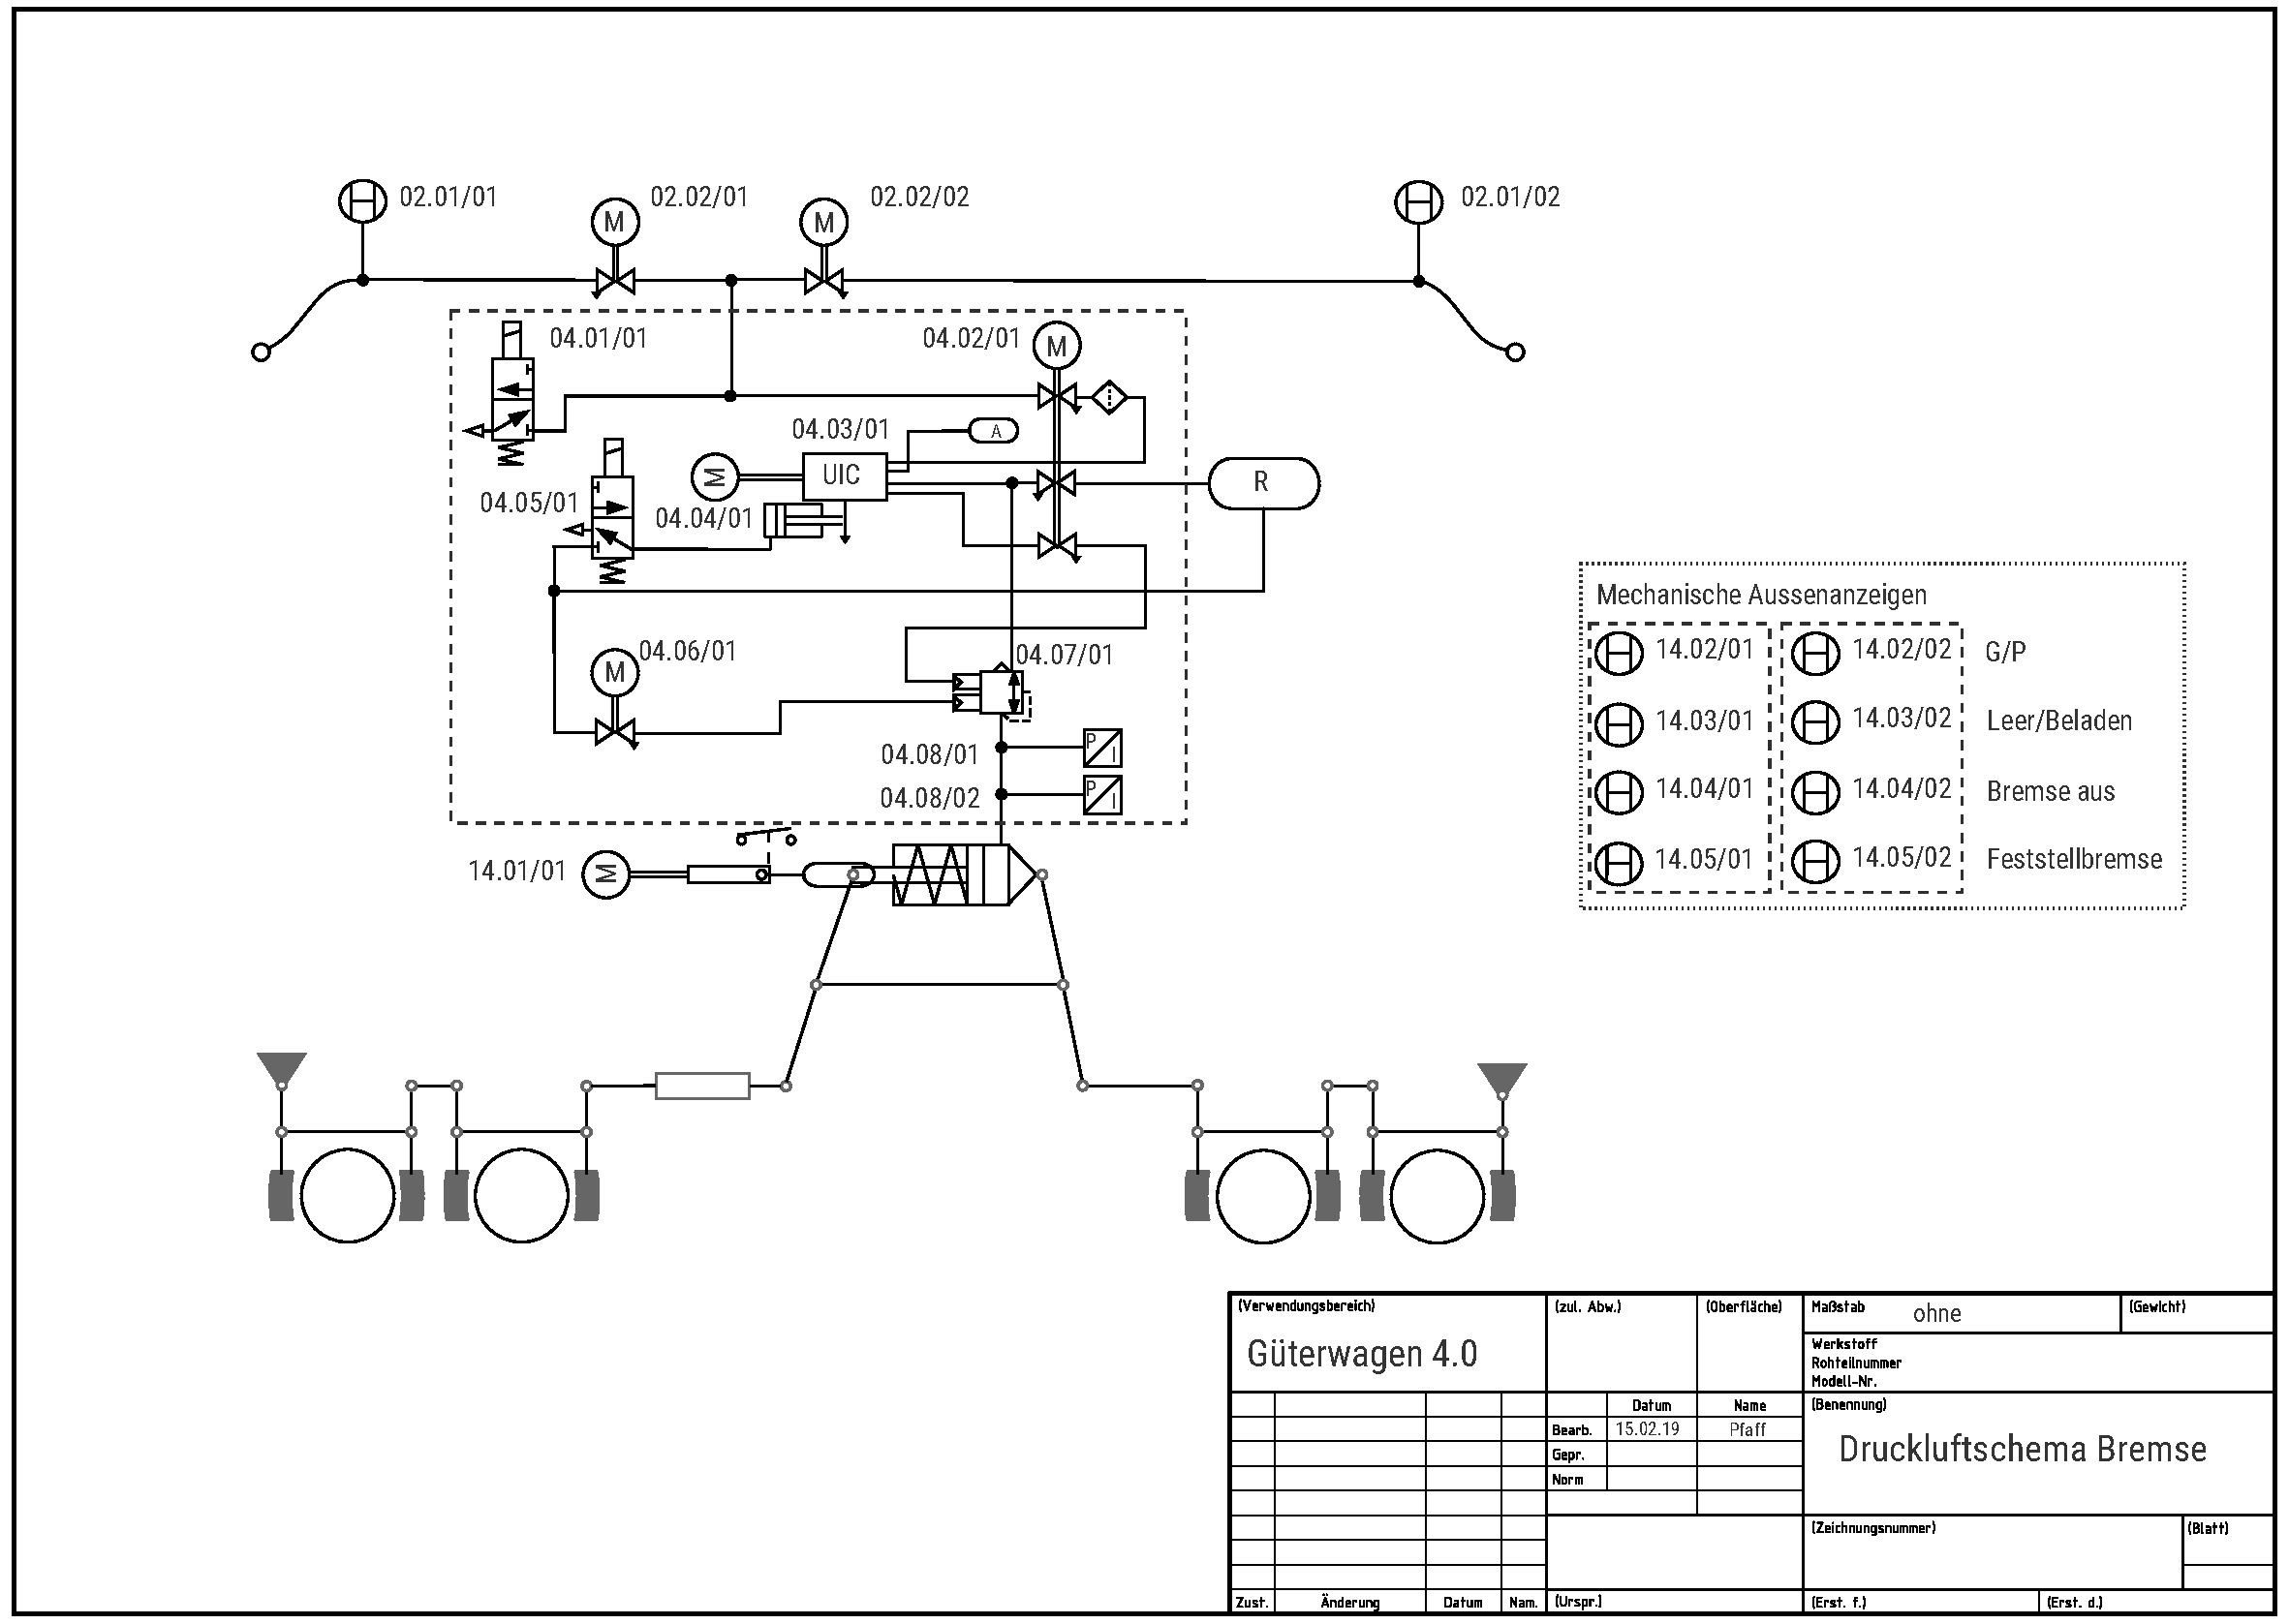
\includepdf[landscape=true, pages=-]{Bilder/PneumaticScheme.pdf} \label{fig:DLS4.0}
\newpage
    \section{Bremse 4.0}
Die Bremse 4.0 blabla 
Das Druckluftschema der \gls{Bremse 4.0} ist in Abbildung \ref{fig:GW40Schema} zu sehen.\par
\begin{figure}[hbt]
    \centering
    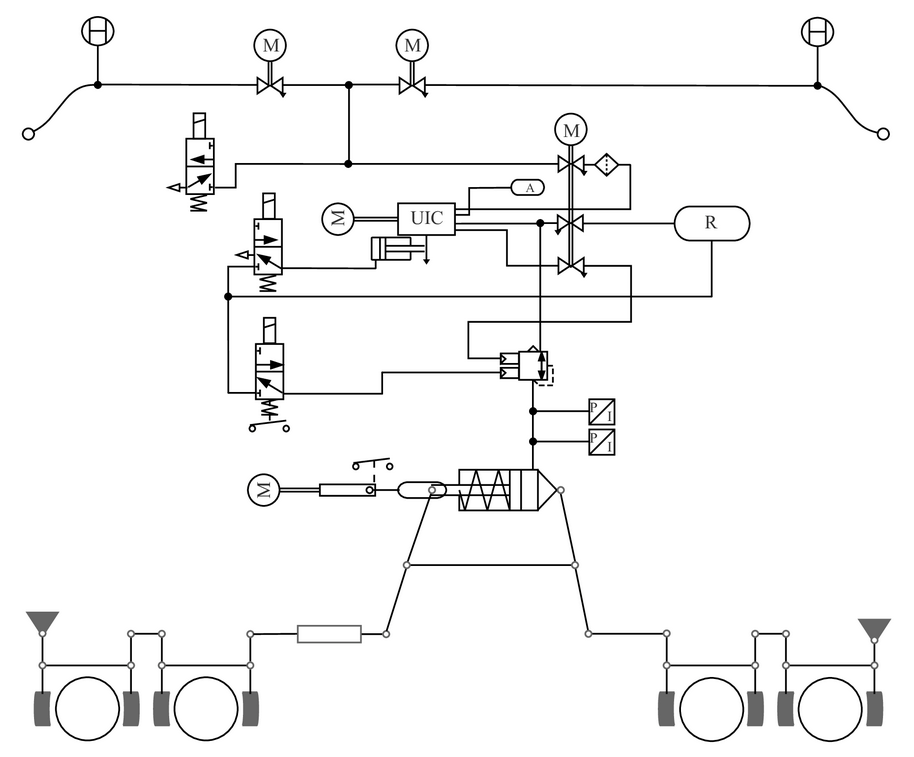
\includegraphics[width=\textwidth]{Bilder/GW40Schema.png}
    \caption{Schema der Güterwagen 4.0 Bremse - Bremse 4.0}
    \label{fig:GW40Schema}
\end{figure}
Für die FMEA-Anlyse wird eine Struktur- und Funktionsanalyse der einzelnen Bauteile benötigt. 

\subsection{Strukturanalayse}
\gls{Bremse 4.0} des Demonstrators.\par
Bauteile die Untersucht werden sollen.\par
Legende: \\
- Komponente des konventionellen \gls{Güterwagens}, die unverändert bleibt\\
+ Komponente des konventionellen \gls{Güterwagens}, die zu einer 4.0-Komponente wird\\
\** Komponente des Güterwagen 4.0, die es nicht im konventionellen Güterwagen gibt\par
\begin{itemize}
    \item[-] Hauptluftleitung
    \begin{itemize}
        \item[+] Endabsperrhahn oder Muffenkugelhahn
        \item[+] Schauzeichen (Anzeige Druck)
        \item[-] Schlauchkupplung
        \item[-] Abzweigung HL-Steuerventil
    \end{itemize}
    \item[+] Steuerventil 4.0
    \begin{itemize}
        \item[-] UIC-konformes Steuerventil
        \item[-] A-Kammer (eventuell Bestandteil des Steuerventil)
        \item[+] G/P-Umstellvorrichtung
        \begin{itemize}
            \item[+] Visuelle Zustandsanzeige mit mechanischer Umsetzung
        \end{itemize}
        \item[+] Schnelllösen
        \item[+] Bremse aus
        \begin{itemize}
            \item[+] Visuelle Zustandsanzeige mit mechanischer Umsetzung
        \end{itemize}
    \end{itemize}
    \item[-] Relaisventil\footnote{Druckübersetzung: aus $C_v$-Druck wird Leistungsdruck}
    \begin{itemize}
        \item[-] Stufenweise Lastwechselumstelleinrichtung
        \begin{itemize}
            \item[+] Visuelle Zustandsanzeige
        \end{itemize}
        \item[+] Vorsteuerventil mit Rückmeldeschalter zur Lasteinstellung\footnote{bestromt=beladen; unbestromt=unbeladen}
    \end{itemize}
    \item[\textasteriskcentered] C-Druck-Sensor\footnote{Für Bremsprobe (siehe Triebzug); Zwischen Relaisventil und Zylinder}
    \item[-] Bremsgestänge\footnote{Lastwechsel wird ausgebaut}
    \item[-] Verschleisnachsteller
    \item[+] Feststellbremse\footnote{Automatische Ablaufbremse ,öglich, Motor mit Kurbel, stetig gebremst, Anlegezeit erstmal zweitrangig}
    \begin{itemize}
        \item[+] Stellantrieb
        \item[-] mechanische Übersetzung
        \item[\textasteriskcentered] Rückmeldeschalter\footnote{für sichere Fahrt: vollständig gelöst, für sicher gebremst: angeschriebenes Handbremsgewicht wird erreicht: 10 Umdrehungen vom gelösten Zustand; dazwischen undefiniert}
        \begin{itemize}
            \item[\textasteriskcentered] Visuelle Anzeige\footnote{Weg der Spindel; Rot, undefiniert, grün}
        \end{itemize}
    \end{itemize}
    \item[\textasteriskcentered] ep-Bremsen\footnote{Entlüftet die HL lokael; elektrische Ansteuerung, indirekte ep-Bremsenfunktion - Vordermann bremst, bremse ich auch, kein ep-lösen, pneumatisches 2-Wege-Ventil}
\end{itemize}

\subsection{Funktionsanalyse}
Funktionen für Zustandsänderugnen an der \gls{Bremse 4.0}
\begin{fkt} \textbf{Feststellbremse}:
\begin{itemize}
    \item gewünschte Bremskraft herstellen / Fahrzeug an einem gewählten Ort auf eine gewünschte Geschwindigkeit verzögern
    \item Fahrzeug dauerhaft gegen wegrollen sichern
    \item lösen
\end{itemize}
\end{fkt}

\begin{fkt} \textbf{Hauptluftleitung}:
\begin{itemize}
    \item Durchleiten der Brems- und Löseanforderung
    \item Einhalten der definierten Leckrate
    \item Energieversorgung der pneumatischen Bremse
    \item Druckfreiheit der Schlauchkupplungen gewährleisten
    \item HL verbinden und absperren
\end{itemize}
\end{fkt}

\begin{fkt} \textbf{Relaisventil}:
\begin{itemize}
    \item Anpassung des Drucks an das Wagengewicht
    \item Leistungsverstärkung anzeigen
    \item Lastwechseleinstellung
\end{itemize}
\end{fkt}

\begin{fkt} \textbf{C-Druck}:
\begin{itemize}
    \item Bremszylinderdruck messen
\end{itemize}
\end{fkt}

\begin{fkt} \textbf{Bremsgestänge}:
\begin{itemize}
    \item gleichmäßige Kraftübertragung auf Räder
    \item VErschleiß nachstellen
\end{itemize}
\end{fkt}

\begin{fkt} \textbf{ep-Bremsen}:
\begin{itemize}
    \item HL lokal entlüften
    \item HL lokal absenken
\end{itemize}
\end{fkt}

\begin{fkt} \textbf{Steuerventil 4.0}
\begin{itemize}
    \item Referenzdruck vorhalten
    \item A-Kammer entlüften
    \item Füll- und Lösezeiten einstellen
    \item lokalen Druckluft-Vorrat speichern
    \item $C_v$-Druck auf $f(a, HL, t, ..)$ einstellen
    \item Steuerventil von HL trennen
    \item \gls{Bremsart} anzeigen
\end{itemize}
\end{fkt}
%Anhang Ende
\end{comment}
\end{document}